\chapter{Introduction}

\section{Install the packages}

\section{The simplest way}
I prepared a VirtualBox disk image \cite{VIRTUALBOX} with a Debian distribution 
and all the required packages. VirtualBox is available for Windows, Linux, 
OS X and Solaris. All the features described in this document are available.

Please contact me via email to receive the link to the zipped file.

\section{Linux}

\subsection{Required packages}

The required modules can be simply installed using the usual package manager 
of the Linux distribution.
It is also possible to install the Anaconda distribution~\cite{ANACONDA} for 
Linux to get the basic Python modules.

It is important to check the versions of the Python modules, in particular 
numpy, scipy and sympy. Old versions of these packages don't allows to perform 
all the tasks described in this document.
In case of old versions, it is possible to download the last versions of these 
packages 
from the SciPy download page~\cite{SCIPYDOWNLOAD}, and install them from a 
Linux 
shell.

Under Debian jessie we can use the apt manager to install the 
following packages:
\begin{itemize}
\item python-numpy (Vers. $\geq$ 1.8.2)
\item python-scipy (Vers. $\geq$ 0.14)
\item python-matplotlib 
\item python-sympy (Vers. $\geq$ 0.7.5)
\item python-setuptools
\item python-psutils
\item jupyter
\item jupyter-qtconsole
\end{itemize}

Under Debian and Ubuntu it is possible to check if all the required development 
packages are correctly installed using the shell command

\begin{verbatim}
sudo apt-get build-dep python-scipy
\end{verbatim}

The following packages are not available as distribution packages and should be 
installed separately.

\begin{itemize}
\item The Python Control toolbox \cite{PYCONTROL}
\item The Slycot libraries \cite{SLYCOT}
\item The pycontrol.tgz package \cite{SUPSICTRL}
\end{itemize}

For the second part of the project (code generation etc.) the following 
packages 
are required

\begin{itemize}
\item python-pyqt4
\item python-pyqt4-dev
\item python-qwt5-qt4
\end{itemize}

This features presented in the second part of this document are at present only 
interesting under the Linux OS, because the real-time code is generated for a 
Linux PREEMPT-RT machine.

\subsection{Install the pycontrol.tgz package}
After downloading the pycontrol.tgz package, unpack it for example under 
``/usr/local'' and you obtain a new folder ``pycontrol''.

The installation is quite simple. Launch as superuser the command

\begin{verbatim}
make
\end{verbatim}

or

\begin{verbatim}
make reduced
\end{verbatim}

if you don't want to have COMEDI installed.

The installation download the control-master package, the slycot-master package 
and install the full software.

As last step it is important to update the ``.bashrc'' file as normal user with 
the command

\begin{verbatim}
make user
\end{verbatim}

The system has been tested under ``Debian stable'', ``Debian testing'' with 
python-2.7, python-3.5 and python-3.6.

\section{Windows}

Under Windows it is sufficient to install the ``Anaconda'' 
package~\cite{ANACONDA}, to have all the python and jupyter modules installed.
The Slycot libraries for Windows can be downloaded from here~\cite{SLYCOT2}.

At present it is not possible to perform hybrid simulation and code generation 
under the Windows OS.

\section{Mac OSX}

The Anaconda package~\cite{ANACONDA} is available for Mac OSX. The Slycot 
libraries can be downloaded from here~\cite{SLYCOT2}.

\chapter{Python - Some hints for Matlab users}

\section{Basics}
There are important differences between Matlab and Python.
In particular, the Python approach to matrices and to indexed objects is 
quite different compared to Matlab.

More information about a comparison between Python and Matlab is available 
online at~\cite{PYTHONVSMATLAB}.

The web contains a lot of documentation about Python and its packages.
In particular, the book of David Pine~\cite{PYMAN} gives a good introduction 
about the features of Python for scientific applications.

Other links present tutorials for \textbf{numpy}~\cite{NUMPY},
\textbf{scipy}~\cite{SCIPY}, \textbf{matplotlib}~\cite{MATPLOTLIB} and 
\textbf{sympy}~\cite{SYMPY}.

\section{The python shell}
A Python script can run within a Python shell, but can also be launched as
executable.

The basic python shell is similar to the Matlab shell without the java 
improvements (\textbf{matlab -nojvm}).

A better shell is for example \textbf{jupyter}. In this interactive form, when 
started as \textbf{jupyter-qtconsole}, jupyter already loads at startup 
a set of functions and modules. 

Another interesting environment, more similar to the Matlab shell, is 
represented by the \textbf{Spyder} application. In this application it is 
possible to debug scripts and functions like in the Matlab environment.

In this document we are mostly working with \textbf{jupyter} launched with the 
shell 
commands

\begin{verbatim}
jupyter-qtconsole
\end{verbatim}

Sometimes not all the functions and modules are explicitly loaded at the 
beginning of the examples. In addition, \textbf{jupyter} implements some useful 
commands like for example \textbf{whos} and \textbf{run} (for launching 
scripts).

In the jupyter shell it is possible to start single commands, paste a set of 
commands or launch a ``.py'' program using \textbf{run}.

\begin{code}
In [1]: # single command

In [2]: a = 5

In [3]: # paste a set of commands

In [4]: a=5
   ...: b=7
   ...: c=a*b
   ...: print c
   ...: 
35

In [5]: # run a .py file

In [6]: run DCmotorKane.py
Matrix([[-Dm*w(t) + kt*I(t)]])
Matrix([[-J*Derivative(w(t), t)]])
[[0 1]
 [0 -Dm/J]]
[[0]
 [kt/J]]
\end{code}

\section{Python vs. Matlab}

Differently from Matlab, Python implements more types of variables

\begin{code}
In [1]: a=5

In [2]: b=2.7

In [3]: c=[[1,2,3],[4,5,6]]

In [4]: d='Ciao'

In [5]: whos
Variable   Type     Data/Info
-----------------------------
a          int      5
b          float    2.7
c          list     n=2
d          str      Ciao
\end{code}


\section{List, array and matrix}
Python implements three kind of multidimensional objects: \textbf{list}, 
\textbf{array} and \textbf{matrix}. 
These objects are handled differently than in Matlab.

\section{List}
A Python \textbf{list} implements the Matlab \textbf{cell}. It represents 
the simplest and default indexed object. 

\begin{code}
In [1]: a=[[[1,2],[3,4]],'abcd',2]

In [2]: b=[[1,2,3],[4,5,6],[7,8,9]]

In [3]: whos
Variable   Type    Data/Info
----------------------------
a          list    n=3
b          list    n=3
\end{code}


\section{Arrays}
In Python the \textbf{array} is a multidimensional variable that implements 
sets of values of the same type. Usually the elements of an array are numbers, 
but can also be booleans, strings, or other objects. An array is the basic 
instance for most scientific applications.

Operations like \textbf{*}, \textbf{/}, \textbf{**} 
etc. implement the \textbf{dot} operations of the Matlab environment 
(\textbf{.*}, \textbf{./} and \textbf{.\^}).
For example, the multiplication of two arrays $a*a$ represents the 
value-by-value multiplication implemented in Matlab with the operation $a.*a$.

\begin{code}
In [1]: from numpy import mat, matrix, array

In [2]: a=array([[1,2,3],[4,5,6]])

In [3]: b=array([[1],[2]])

In [4]: print a*a
[[ 1  4  9]
 [16 25 36]]

In [5]: print a*b
[[ 1  2  3]
 [ 8 10 12]]
\end{code}

\section{Matrices}
The \textbf{matrix} object is useful in case of linear algebra operations.
In this case the variables are instanced using the \textbf{mat} or the
\textbf{matrix} function.

\begin{code}
In [1]: from numpy import mat, matrix, array

In [2]: a=mat(a)

In [3]: b=array([[1],[2],[3]])

In [4]: a*b
Out[5]: 
matrix([[14],
        [32]])

In [6]: a=array(a)
\end{code}

\begin{code}
In [7]: a*b
----------------------------------------------
ValueError			Traceback (most recent call last)
<ipython-input-9-8201c27d19b7> in <module>()
----> 1 a*b

ValueError: operands could not be broadcast together with shapes (2,3) (3,1) 

In [8]: b=mat(b)

In [9]: a*b
Out[10]: 
matrix([[14],
        [32]])
\end{code}

\section{Indexing}
Indexing in Python is quite different compared with the syntax used in Matlab.
Indices start from \textbf{0} (and not \textbf{1} as in Matlab).
In addition, the syntax is different for lists, arrays and matrices.

\section{Lists}
1-dimension lists can be accessed using one index (ex. $a[2]$). Multidimensional
lists require multiple indices in the form $[i][j]$\ldots

\begin{code}
In [1]: a=[1,2,3,4,5]

In [2]: %whos
Variable   Type    Data/Info
----------------------------
a          list    n=5

In [3]: a[3]
Out[3]: 4

In [4]: b=[[1,2,3],[4,5,6]]

In [5]: %whos
Variable   Type    Data/Info
----------------------------
a          list    n=5
b          list    n=2

In [6]: b[1][2]
Out[6]: 6

In [7]: b[0]
Out[7]: [1, 2, 3]
\end{code}

\section{Arrays}
Multidimensional arrays allow the use of indices in the forms $[i,j]$ and 
$[i][j]$.

\begin{code}
In [1]: from numpy import array

In [2]: a=array([1,2,3,4,5])

In [3]: b=array([[1,2,3],[4,5,6]])

In [4]: %whos
Variable   Type       Data/Info
-------------------------------
a          ndarray    5: 5 elems, type `int64`, 40 bytes
b          ndarray    2x3: 6 elems, type `int64`, 48 bytes
\end{code}

\begin{code}
In [5]: a.shape
Out[5]: (5,)

In [6]: b.shape
Out[6]: (2, 3)

In [7]: a[3]
Out[7]: 4

In [8]: b[0,2]
Out[8]: 3

In [9]: b[0][2]
Out[9]: 3

In [10]: b[:,0]
Out[10]: array([1, 4])

In [11]: b[0,:]
Out[11]: array([1, 2, 3])

In [12]: b[0]
Out[12]: array([1, 2, 3])
\end{code}

\section{Matrices}
Matrices can be only indexed using the $[i,j]$ syntax. A matrix has always a 
minimum of 2 dimensions.

\begin{code}
In [1]: from numpy import mat

In [2]: a=array([1,2,3,4,5])

In [3]: b=array([[1,2,3],[4,5,6]])

In [4]: %whos
Variable   Type      Data/Info
------------------------------
a          matrix    [[1 2 3 4 5]]
b          matrix    [[1 2 3]\n [4 5 6]]

In [5]: a.shape
Out[5]: (1, 5)

In [6]: b.shape
Out[6]: (2, 3)
\end{code}

\begin{code}
In [7]: a[0,2]
Out[7]: 3

In [8]: b[1,1]
Out[8]: 5

In [9]: b[:,0]
Out[9]: 
matrix([[1],
        [4]])

In [10]: b[0,:]
Out[10]: matrix([[1, 2, 3]])
\end{code}

\section{Multidimensional arrays and matrices}
Matrices and arrays can be defined with more than 2 dimensions.

\begin{code}
In [1]: from numpy import array, mat

In [2]: a=zeros((3,3,3),int8)

In [3]: a.shape
Out[3]: (3, 3, 3)

In [4]: %whos
Variable   Type       Data/Info
-------------------------------
a          ndarray    3x3x3: 27 elems, type `int8`, 27 bytes

In [5]: a[1,1,1]
Out[5]: 0
In [6]: a[1,1,1]=5

In [7]: a
Out[7]: 
array([[[0, 0, 0],
        [0, 0, 0],
        [0, 0, 0]],

       [[0, 0, 0],
        [0, 5, 0],
        [0, 0, 0]],

       [[0, 0, 0],
        [0, 0, 0],
        [0, 0, 0]]], dtype=int8)

\end{code}

% \section{Other differences between lists, arrays and matrices}
% 
% In the next example we can see another difference between the 3 objects.
% 
% \begin{code}
% In [1]: a=[1,2,3]
% 
% In [2]: whos
% Variable   Type    Data/Info
% ----------------------------
% a          list    n=3
% 
% In [3]: 2*a	# list
% Out[3]: [1, 2, 3, 1, 2, 3]
% 
% In [4]: 2*array(a)	# array
% Out[4]: array([2, 4, 6])
% 
% In [5]: 2*mat(a)	# matrix
% Out[5]: matrix([[2, 4, 6]])
% \end{code}

\newpage

\chapter{The Python Control System toolbox}
\section{Basics}

The Python Control Systems Library, is a package initially developed by 
Richard Murray at Caltech. This toolbox  contains a set of python classes 
and functions that implement common operations for the analysis and design of 
feedback control systems. 
In addition, a MATLAB compatibility package (control.matlab) has been 
integrated in order to provide functions equivalent to the commands available 
in the MATLAB Control Systems Toolbox.

\section{Models}

LTI systems can be described in state-space form or as transfer functions.

\section{Continuous systems}
\section{State-space representation}
\begin{code}
In [1]: from control import *

In [2]: a=[[0,1],[-1,-1]]

In [3]: b=[[0],[1]]

In [4]: c=[1,0]

In [5]: d=0

In [6]: sys = ss(a,b,c,d)

In [7]: print sys
A = [[ 0  1]
 [-1 -1]]

B = [[0]
 [1]]

C = [[1 0]]

D = [[0]]
\end{code}

 
\section{Transfer function}

\begin{code}
 In [1]: from control import *

In [2]: g=tf(1,[1,1,1])

In [3]: print g

     1
-----------
s^2 + s + 1
\end{code}


\section{Zeros-Poles-Gain}
This method is not implemented in control toolbox yet. It is available in the 
package \textbf{scipy.signal} but it is not completely compatible with the 
class of LTI objects defined in the Python control toolbox.

\section{Discrete time systems}
An additional fields (\textbf{dt}) in the \textbf{StateSpace} and 
\textbf{TransferFunction} classes is used to differentiate continuous-time and 
discrete-time systems.

\section{State-space representation}
\begin{code}
In [4]: a=[[0,1],[-1,1]]

In [5]: b=[[0],[1]]

In [6]: c=[1,-1]

In [7]: d=0

In [8]: sysd = ss(a,b,c,d,0.01)

In [9]: print sysd
A = [[ 0  1]
 [-1  1]]

B = [[0]
 [1]]

C = [[ 1 -1]]

D = [[0]]

dt = 0.01
\end{code}


\section{Transfer function}
\begin{code}
In [1]: from control import *

In [2]: g=tf([1,-1],[1,-1,1],0.01)

In [3]: print g

   z - 1
-----------
z^2 - z + 1

dt = 0.01
\end{code}

\section{Conversions}

The Python control system toolbox only implements conversion from continuous 
time systems to discrete-time systems ( \textbf{c2d} ) with the methods 
``zoh'', ``tustin'' and ``matched''. No conversion from discrete to continuous 
has been implemented yet.

The supsictrl.ctr\_repl package implements both functions \textbf{c2d} and 
\textbf{d2c} with the methods ``zoh', ''foh``, ''tustin`` and ''matched`` 
(''matched`` is only implemented in c2d).

\begin{code}
In [1]: from control import *

In [2]: from control.Matlab import *

In [3]: g=tf(1,[1,1,1])

In [4]  # Matlab compatibility 

In [5]: gd = c2d(g,0.01)             

In [6]  # control toolbox 

In [7]: gd2 = sample_system(g,0.01)  

In [8]: print g

     1
-----------
s^2 + s + 1


In [9]: print gd

4.983e-05 z + 4.967e-05
-----------------------
  z^2 - 1.99 z + 0.99

dt = 0.01
\end{code}

\begin{code}
In [1]: from control import *

In [2]: from control.Matlab import c2d

In [3]: from supsictrl.ctrl_repl import d2c

In [4]: g=tf(1,[1,1,1])

In [5]: gd =c2d(g,0.01)

In [6]: g2=d2c(gd)

In [7]: print g

     1
-----------
s^2 + s + 1


In [8]: print g2

1.729e-14 s + 1
---------------
  s^2 + s + 1
\end{code}

\section{Casting}
The control.matlab module implements the casting functions to transform LTI 
systems to a transfer function (\textbf{tf}) or to a state-space form 
(\textbf{ss}).

\begin{code}
In [8]: g = tf(sys)

In [9]: print g

     1
-----------
s^2 + s + 1

\end{code}

and transfer functions into one of the  state-space representation

\begin{code}
In [10]: sys = ss(g)

In [11]: print sys
A = [[ 0. -1.]
 [ 1. -1.]]

B = [[-1.]
 [ 0.]]

C = [[ 0. -1.]]

D = [[ 0.]]

\end{code}
\section{Models interconnection}

Commands like \textbf{parallel} and \textbf{series} are available in order to 
interconnect systems. The operators \textbf{+} and \textbf{*} have been 
overloaded for the LTI class to perform the same operations. In addition the 
command \textbf{feedback} is implemented exactly as in Matlab.

\begin{code}
In [1]: from control import *

In [2]: g1=tf(1,[1,1])

In [3]: g2=tf(1,[1,2])

In [4]: print parallel(g1,g2)

   2 s + 3
-------------
s^2 + 3 s + 2


In [5]: print g1+g2

   2 s + 3
-------------
s^2 + 3 s + 2
\end{code}

\begin{code}
In [6]: print series(g1,g2)

      1
-------------
s^2 + 3 s + 2


In [7]: print g1*g2

      1
-------------
s^2 + 3 s + 2
\end{code}

\begin{code}
In [8]: print feedback(g1,g2)

    s + 2
-------------
s^2 + 3 s + 3
\end{code}

\chapter{System analysis}

\section{Time response}

The Python Control toolbox offers own functions to simulate the time 
response of systems. For Matlab users, the control.matlab module gives the 
possibility to work with the same syntax as in Matlab.
Please take care about the order of the return values!

Examples of time responses are shown in the figures~\ref{F1}, \ref{F2}, 
\ref{F3}, \ref{F4} and~\ref{F5}.

\begin{figure}[htbp]	% Step
\begin{minipage}[t]{0.55\textwidth}
  \vspace{0pt}
\begin{lstlisting}[linewidth=7cm, xleftmargin=0cm]
In [1]: from control import *

In [2]: import matplotlib.pyplot as plt

In [3]: g = tf(1,[1,1,1])

In [4]: t,y = step_response(g)

In [5]: plt.plot(t,y)
   ...: plt.grid()
   ...: plt.xlabel('t')
   ...: plt.ylabel('y')

\end{lstlisting}

or alternatively

\begin{lstlisting}[linewidth=7cm,xleftmargin=0cm]
In [1]: from control import *

In [2]: from control.matlab import *

In [3]: import matplotlib.pyplot as plt

In [4]: g = tf(1,[1,1,1])

In [5]: y,t = step(g)

In [6]: plt.plot(t,y)
   ...: plt.xlabel('t')
   ...: plt.ylabel('y')
   ...: plt.grid()
\end{lstlisting}
\end{minipage}%
\begin{minipage}[t]{0.45\textwidth}
  \centering
  \vspace{0.2cm}
  \includegraphics[width=\textwidth]{eps/stepresp.eps}
\end{minipage}
\caption{Step response for continuous-time systems}
\label{F1}
\end{figure}

\begin{figure}[htbp]	%discrete step
\begin{minipage}[t]{0.55\textwidth}
  \vspace{0pt}
\begin{lstlisting}[linewidth=7cm,xleftmargin=0cm]
In [1]: from control import *

In [2]: from control.matlab import c2d

In [3]: import matplotlib.pyplot as plt

In [4]: g = tf(1,[1,1,1])

In [5]: gz=c2d(g,0.1)

In [6]: t=arange(0,16,0.1)

In [7]: t1,y = step_response(gz,t)

In [8]: plt.step(t,y.T[0]) # transpose col matrix y[0]
   ...: plt.grid()
   ...: plt.xlabel('t')
   ...: plt.ylabel('y')
\end{lstlisting}

or alternatively

\begin{lstlisting}[linewidth=7cm,xleftmargin=0cm]
In [1]: from control import *

In [2]: from control.matlab import *

In [3]: import matplotlib.pyplot as plt

In [4]: g = tf(1,[1,1,1])

In [5]: gz=c2d(g,0.1)

In [6]: t=arange(0,16,0.1)

In [7]: y,t1 = step(gz,t)

In [8]: plt.step(t,y[0])  # get first row from y matrix
   ...: plt.grid()
   ...: plt.xlabel('t')
   ...: plt.ylabel('y')
\end{lstlisting}
\end{minipage}%
\begin{minipage}[t]{0.5\textwidth}
  \vspace{0pt} \centering
  \includegraphics[width=\textwidth]{eps/dstepresp.eps}
\end{minipage}
\caption{Step response for discrete-time systems}
\label{F2}
\end{figure}

\begin{figure}[htbp]	% initial
\begin{minipage}[t]{0.55\textwidth}
  \vspace{0pt}
\begin{lstlisting}[linewidth=7cm,xleftmargin=0cm]
In [1]: from control import *

In [2]: import matplotlib.pyplot as plt

In [3]: a=[[0,1],[-1,-1]]

In [4]: b=[[0],[1]]

In [5]: c=[1,0]

In [6]: d=[0]

In [7]: sys=ss(a,b,c,d)

In [8]: t,y=initial_response(sys,
                             X0=[1,1])

In [9]: plt.plot(t,y)
   ...: plt.grid()
   ...: plt.xlabel('t')
   ...: plt.ylabel('y')
\end{lstlisting}

or alternatively

\begin{lstlisting}[linewidth=7cm,xleftmargin=0cm]
In [1]: from control import *

In [2]: from control.matlab import *

In [3]: import matplotlib.pyplot as plt

In [4]: a=[[0,1],[-1,-1]]

In [5]: b=[[0],[1]]

In [6]: c=[1,0]

In [7]: d=[0]

In [8]: sys=ss(a,b,c,d)

In [9]: y,t=initial(sys,X0=[1,1])

In [10]: plt.plot(t,y)
   ...: plt.xlabel('t')
   ...: plt.ylabel('y')
   ...: plt.grid()
\end{lstlisting}
\end{minipage}%
\begin{minipage}[t]{0.5\textwidth}
  \vspace{0pt} \centering
  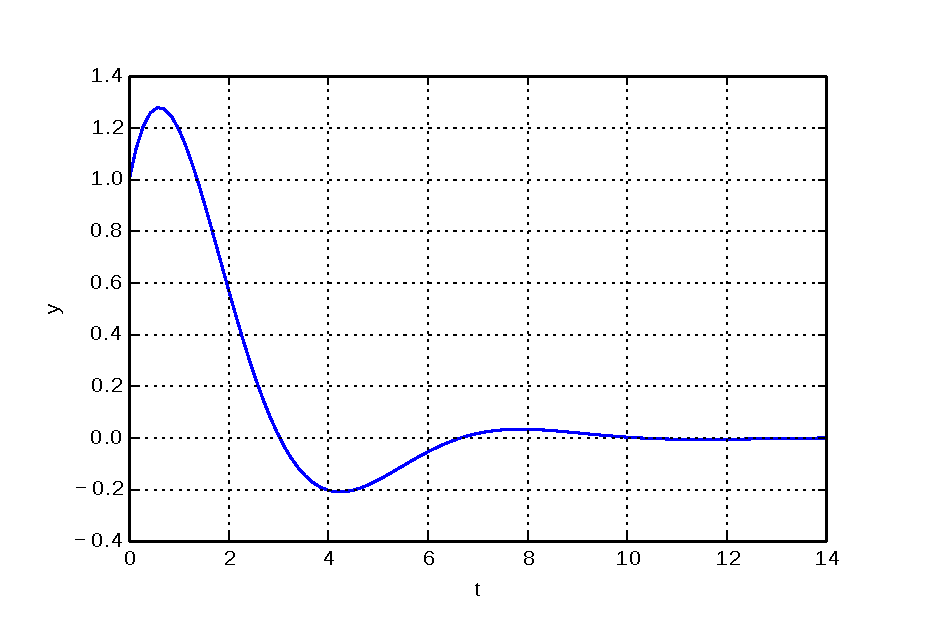
\includegraphics[width=\textwidth]{eps/initial.eps}
\end{minipage}
\caption{Continuous time systems - Initial condition response}
\label{F3}
\end{figure}

\begin{figure}[htbp]	% impulse
\begin{minipage}[t]{0.55\textwidth}
  \vspace{0pt}
\begin{lstlisting}[linewidth=7cm,xleftmargin=0cm]
In [1]: from control import *

In [2]: import matplotlib.pyplot as plt

In [3]: g = tf(1,[1,1,1])

In [4]: t,y = impulse_response(g)

In [5]: plt.plot(t,y)
   ...: plt.grid()
   ...: plt.xlabel('t')
   ...: plt.ylabel('y')
\end{lstlisting}

or alternatively

\begin{lstlisting}[linewidth=7cm,xleftmargin=0cm]
In [1]: from control import *

In [2]: from control.matlab import *

In [3]: import matplotlib.pyplot as plt

In [4]: g = tf(1,[1,1,1])

In [5]: y,t = impulse(g)

In [6]: plt.plot(t,y)
   ...: plt.grid()
   ...: plt.xlabel('t')
   ...: plt.ylabel('y')
\end{lstlisting}
\end{minipage}%
\begin{minipage}[t]{0.5\textwidth}
  \vspace{0pt} \centering
  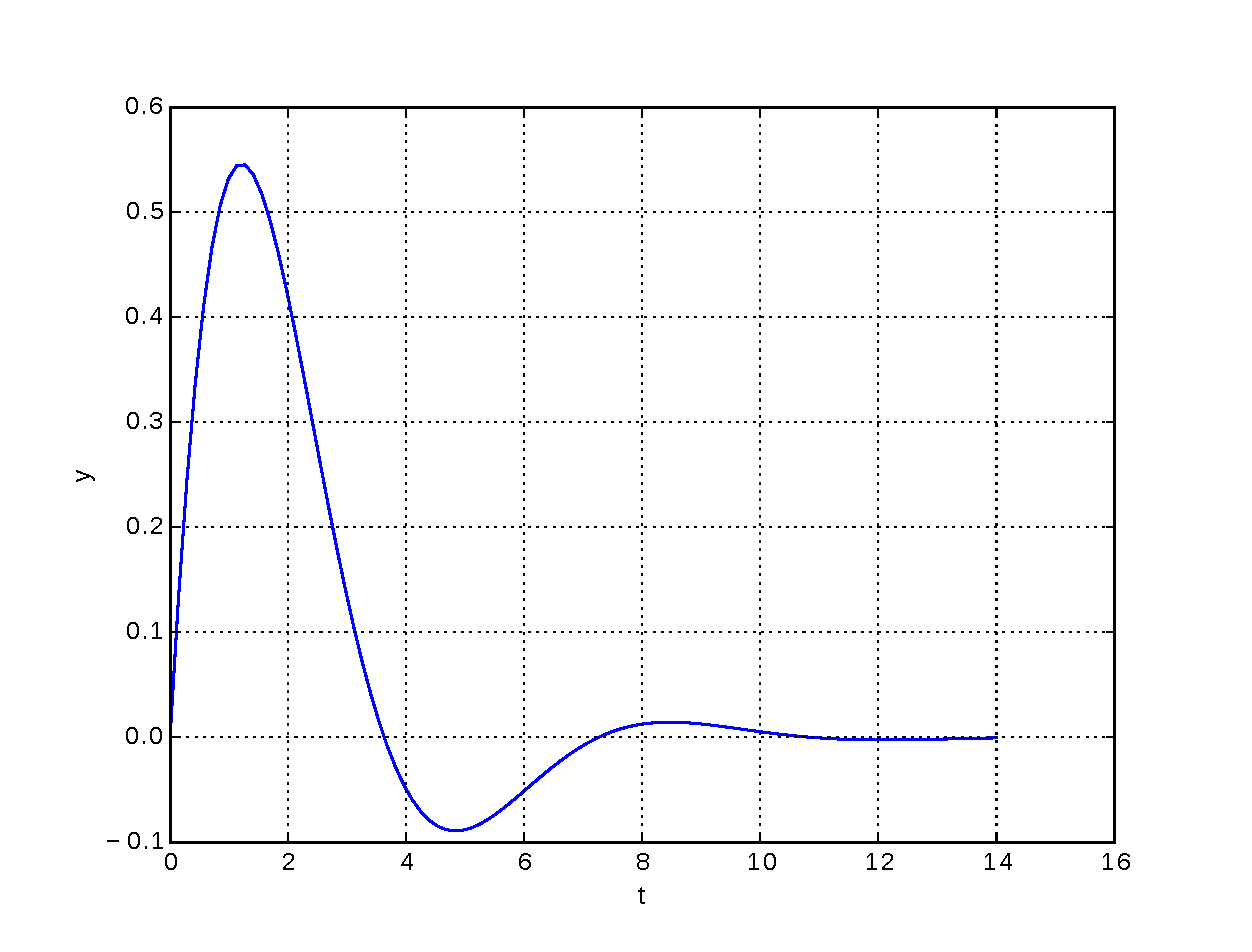
\includegraphics[width=\textwidth]{eps/impulse.eps}
\end{minipage}
\caption{Continuous time systems - Impulse response}
\label{F4}
\end{figure}

\begin{figure}[htbp]  % forced
\begin{minipage}[t]{0.55\textwidth}
  \vspace{0pt}
\begin{lstlisting}[linewidth=7cm,xleftmargin=0cm]
In [1]: from control import *

In [2]: import matplotlib.pyplot as plt

In [3]: g=tf([1,2],[1,2,3,4])

In [4]: t=linspace(0,6*pi)

In [5]: u=sin(t)

In [6]: t,y,x = forced_response(g,t,u)

In [7]: plt.plot(t,y)
   ...: plt.xlabel('t')
   ...: plt.ylabel('y')
   ...: plt.grid()
\end{lstlisting}

or alternatively

\begin{lstlisting}[linewidth=7cm,xleftmargin=0cm]
In [1]: from control import *

In [2]: from control.matlab import *

In [3]: import matplotlib.pyplot as plt

In [4]: g=tf([1,2],[1,2,3,4])

In [5]: t=linspace(0,6*pi)

In [6]: u=sin(t)

In [7]: y,t,x = lsim(g,u,t)

In [8]: plt.plot(t,y)
   ...: plt.xlabel('t')
   ...: plt.ylabel('y')
   ...: plt.grid()
\end{lstlisting}
\end{minipage}%
\begin{minipage}[t]{0.5\textwidth}
  \vspace{0pt} \centering
  \includegraphics[width=\textwidth]{eps/lsim.eps}
\end{minipage}
\caption{Continuous time systems - Generic input}
\label{F5}
\end{figure}

\newpage
\section{Frequency analysis}

The frequency analysis includes some commands like \textbf{bode\_response}, 
\textbf{nyquist\_response}, \textbf{nichols\_response} and the corresponding 
Matlab versions \textbf{bode}, \textbf{nyquist} and \textbf{nichols}. (See 
figures~\ref{F6}, \ref{F7} and~\ref{F8})

\begin{figure}[htbp]
\begin{minipage}[t]{0.55\textwidth}
  \vspace{0pt}
\begin{lstlisting}[linewidth=7cm,xleftmargin=0cm]
In [1]: from control import *

In [2]: g=tf([1],[1,0.5,1])

In [3]: bode_plot(g, dB=True);
\end{lstlisting}

or alternatively

\begin{lstlisting}[linewidth=7cm,xleftmargin=0cm]
In [1]: from control import *

In [2]: from control.matlab import *

In [3]: g=tf([1],[1,0.5,1])

In [4]: bode(g, dB=True);
\end{lstlisting}
\end{minipage}%
\begin{minipage}[t]{0.5\textwidth}
  \vspace{0pt} \centering
  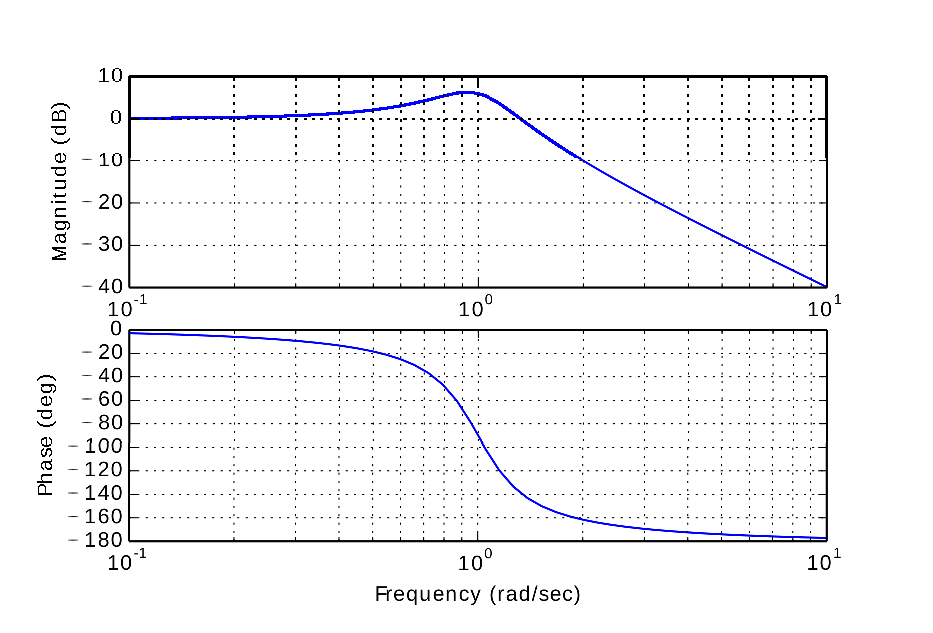
\includegraphics[width=\textwidth]{eps/bode.eps}
\end{minipage}
\caption{Bode plot}
\label{F6}
\end{figure}

\begin{figure}[htbp]
\begin{minipage}[t]{0.55\textwidth}
  \vspace{0pt}
\begin{lstlisting}[linewidth=7cm,xleftmargin=0cm]
In [1]: from control import *

In [2]: import matplotlib.pyplot as plt

In [3]: g=tf([1],[1,2,1])

In [3]: nyquist_plot(g), plt.grid()
\end{lstlisting}

or alternatively

\begin{lstlisting}[linewidth=7cm,xleftmargin=0cm]
In [1]: from control import *

In [2]: import matplotlib.pyplot as plt

In [3]: from control.matlab import *

In [4]: g=tf(1,[1,2,1])

In [5]: nyquist(g), plt.grid()
\end{lstlisting}

\end{minipage}%
\begin{minipage}[t]{0.5\textwidth}
  \vspace{0pt} \centering
  \includegraphics[width=\textwidth]{eps/nyquist.eps}
\end{minipage}
\caption{Nyquist plot}
\label{F7}
\end{figure}

\begin{figure}[htbp]
\begin{minipage}[t]{0.55\textwidth}
  \vspace{0pt}
\begin{lstlisting}[linewidth=7cm,xleftmargin=0cm]
In [1]: from control import *

In [2]: g=tf(1,[1,2,3,4,0])

In [3]: nichols_plot(g)
\end{lstlisting}

or alternatively

\begin{lstlisting}[linewidth=7cm,xleftmargin=0cm]
In [1]: from control import *

In [2]: g=tf(1,[1,2,3,4,0])

In [3]: nichols(g)
\end{lstlisting}

\end{minipage}%
\begin{minipage}[t]{0.5\textwidth}
  \vspace{0pt} \centering
  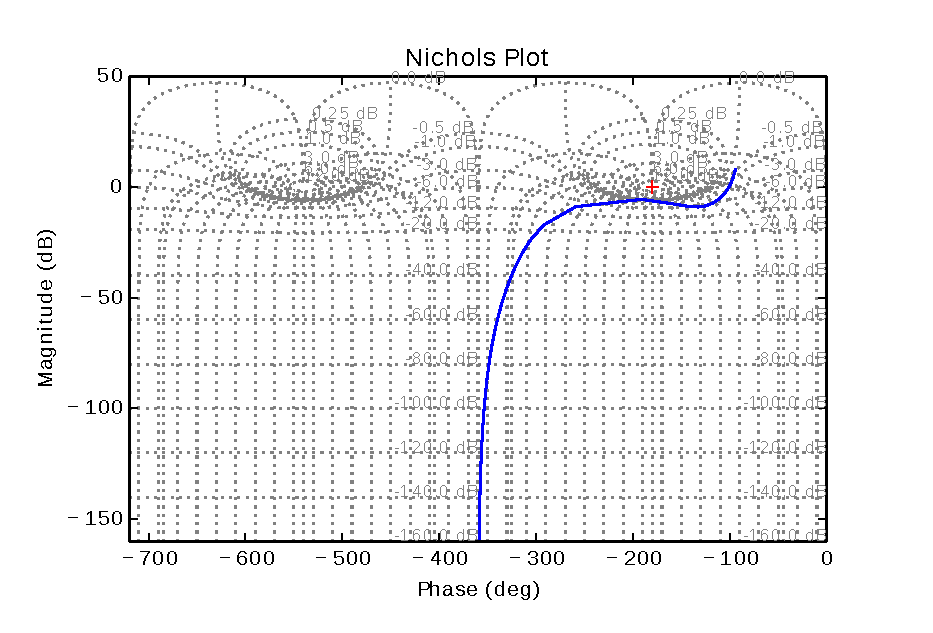
\includegraphics[width=\textwidth]{eps/nichols.eps}
\end{minipage}
\caption{Nichols plot}
\label{F8}
\end{figure}

The command \textbf{margins} returns the gain margin, the phase margin and the 
corresponding crossover frequencies.

\begin{code}
In [1]: from control import *

In [2]: g=tf(2,[1,2,3,1])

In [3]: gm, pm, wg, wp = margin(g)

In [4]: gm			# Gain, not dB!
Out[4]: 2.5000000000000013

In [5]: pm
Out[5]: 76.274075256921392	# deg

In [6]: wg
Out[6]: 0.85864877610167201	# rad/s

In [7]: wp
Out[7]: 1.7320508075688776	# rad/s
\end{code}

In addition, the command \textbf{stability\_margins} returns the stability 
margin and the corresponding frequency. The stability margin values $w_s$ and 
$s_m$, which correspond to the shortest distance from the Nyquist curve to the 
critical point $-1$, are useful for the sensitivity analysis. 

\begin{code}
In [1]: from control import *

In [2]: g=tf(2,[1,2,3,1])

In [3]: gm, pm, sm, wg, wp, ws = stability_margins(g)

In [4]: gm
Out[4]: 2.5000000000000013	# Gain not dB`

In [5]: pm
Out[5]: 76.274075256921392	# deg

In [6]: wg
Out[6]: 1.7320508075688776	# rad/s

In [7]: wp
Out[7]: 0.85864877610167201	# rad/s

In [8]: sm
Out[8]: 0.54497577553096421	#

In [9]: ws
Out[9]: 1.3669371206538097	# rad/s
\end{code}

\section{Poles, zeros and root locus analysis}
Poles and zeros of an open loop system can be calculated with the 
commands \textbf{pole}, \textbf{zero} or plotted and calculated with 
\textbf{pzmap}.

\begin{figure}[htbp]
\begin{minipage}[t]{0.55\textwidth}
  \vspace{0pt}
\begin{lstlisting}[linewidth=7cm,xleftmargin=0cm]
In [1]: from control import *

In [2]: from control.pzmap import pzmap

In [3]: g=tf([1,1],[1,2,3,4,0])

In [4]: g.pole()
Out[4]: 
array([-1.65062919+0.j        , -0.17468540+1.54686889j,
       -0.17468540-1.54686889j,  0.00000000+0.j        ])

In [5]: g.zero()
Out[5]: array([-1.])

In [6]: poles, zeros = pzmap(g), grid()

In [7]: poles

Out[7]: 
array([-1.65062919+0.j        , -0.17468540+1.54686889j,
       -0.17468540-1.54686889j,  0.00000000+0.j        ])

In [8]: zeros
Out[8]: array([-1.])
\end{lstlisting}

\end{minipage}%
\begin{minipage}[t]{0.5\textwidth}
  \vspace{0pt} \centering
  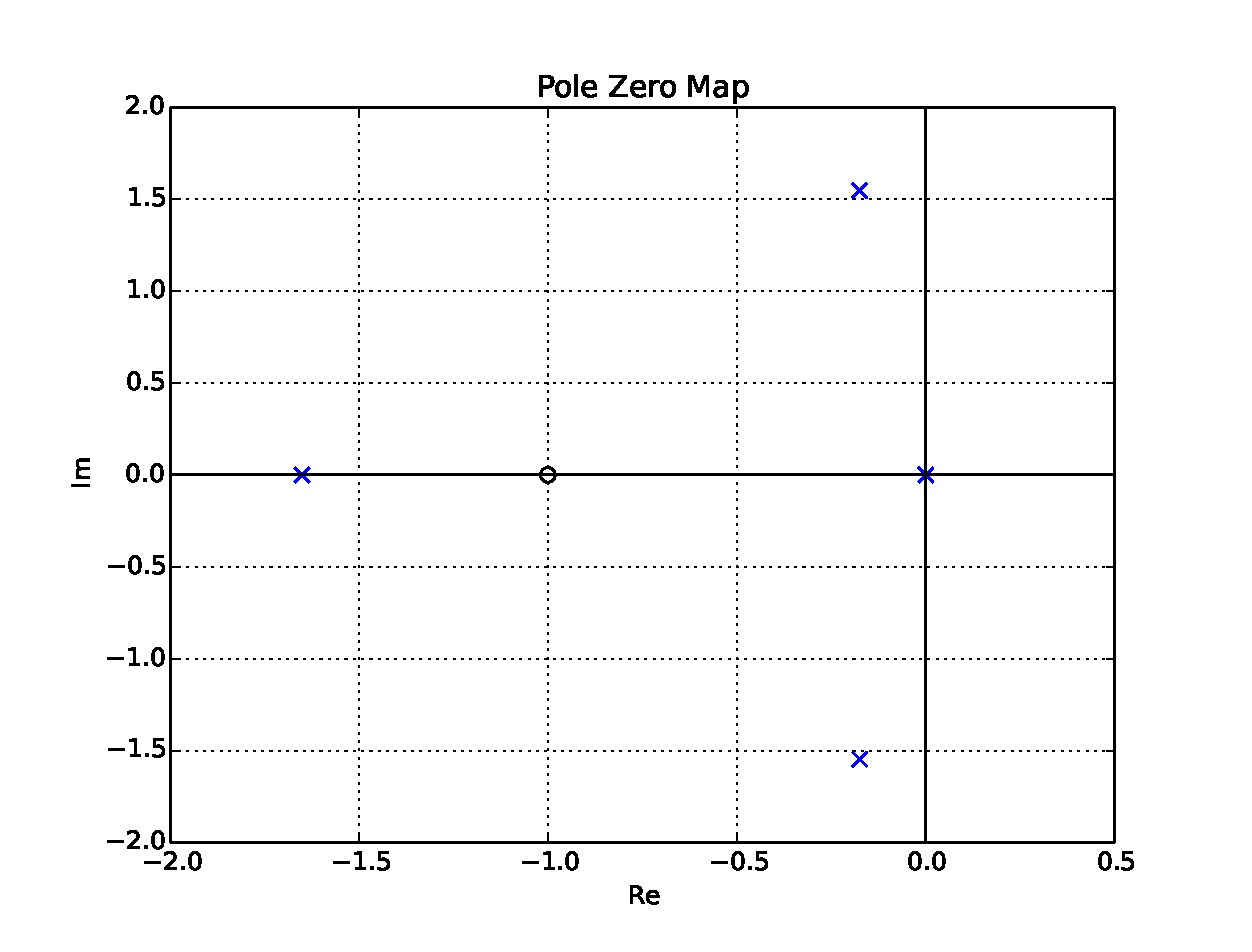
\includegraphics[width=0.9\textwidth]{eps/pzmap.eps}
\end{minipage}
\caption{Poles and zeros}
\label{F8a}
\end{figure}

In addition there are two functions that implement the root locus command: 
\textbf{rlocus} and \textbf{root\_locus}. At present no algorithm to 
automatically choose the values  of $K$ has been implemented: if not provided, 
the $K$ vector is calculated in rlocus with log values between $10^{-3}$ and 
$10^3$. For the \textbf{root\_locus} function the $K$ values should be 
provided. 

\begin{figure}[htbp]
\begin{minipage}[t]{0.55\textwidth}
  \vspace{0pt}
\begin{lstlisting}[linewidth=7cm,xleftmargin=0cm]
In [1]: from control import *

In [2]: g=tf(1,[1,2,3,0])

In [3]: rlocus(g); grid()
\end{lstlisting}

or alternatively

\begin{lstlisting}[linewidth=7cm,xleftmargin=0cm]
In [1]: from control import *

In [2]: g=tf(1,[1,2,3,0])

In [3]: k=logspace(-3,3,100)

In [4]: root_locus(g,k); grid()
\end{lstlisting}

\end{minipage}%
\begin{minipage}[t]{0.5\textwidth}
  \vspace{0pt} \centering
  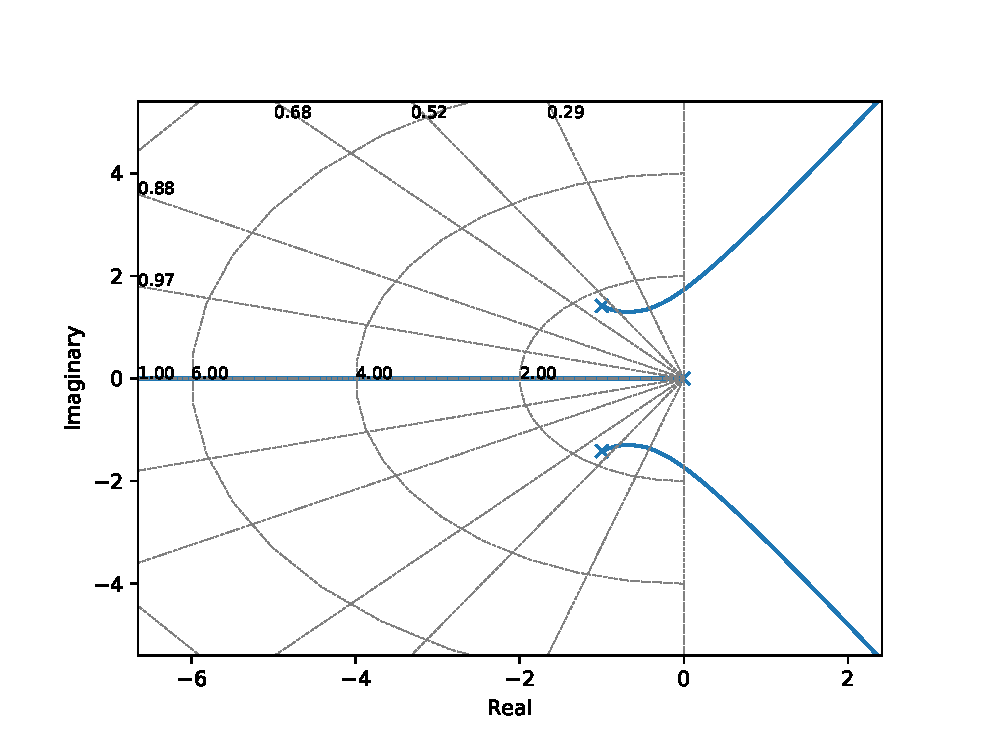
\includegraphics[width=\textwidth]{eps/rlocus.eps}
\end{minipage}
\caption{Root locus plot}
\label{F9}
\end{figure}

If in the jupyter shell you set the command \textbf{\%matplotlib qt}, the root 
locus is plotted on an external window and it is possible to get the values of 
gain and damp by clicking with the mouse on the curves.

\begin{code}
Clicked at    -0.5724    +1.293j gain      1.722 damp     0.4048
Clicked at     -1.119  +0.01874j gain      2.252 damp     0.9999
Clicked at    -0.7545    +1.293j gain      1.114 damp      0.504
\end{code}

\chapter{Modeling}
The \textbf{sympy} module (symbolic python) contains a full set of operations 
to manage physical systems.
In particular,  it is possible to find the linearized model of a 
mechanical system using the Lagrange's method or the Kane's method.
More details about the Kane's method are available at~\cite{KANE1}, 
\cite{KANE2}, \cite{KANE6}, \cite{KANE3}, \cite{KANE4} and~\cite{KANE5}.

In the next sections we present the modelling of 3 plants that we can find in 
our laboratories and that are quite familiar to us.

\section{Model of a DC motor}
\subsection{Plant}
In this first example we model a DC servo motor with a current input in order 
to find its state-space representation. The motor is characterized by a torque 
constant $k_t$, an inertia (motor+load) $J$ and a friction constant $D_m$.

The input of the plant is the current $I$ and the output is the position 
$\varphi$. The rotation center is the point \textbf{O}, the main coordinates 
system is \textbf{N} and we add a local reference frame \textbf{Nr} which 
rotates with the load (angle $\varphi$ and speed $\omega$).

\subsection{Modules and constants}
\begin{code}
n [1]: from sympy import symbols, Matrix,pi
   ...: from sympy.physics.mechanics import *
   ...: import numpy as np
   ...: 
   ...: # Modeling the system with Kane method
   ...: 
   ...: # Signals
   ...: ph = dynamicsymbols('ph')    # motor angle
   ...: w  = dynamicsymbols('w')     # motor rot. speed
   ...: I  = dynamicsymbols('I')     # input current
   ...: 
   ...: # Constants
   ...: Dm = symbols('Dm')           # friction
   ...: M, J = symbols('M J')        # Mass and inertia
   ...: t = symbols('t')             # time
   ...: kt  = symbols('kt')          # torque constant
   ...: 
\end{code}

\subsection{Reference frames}
\begin{code}
In [2]: # Reference frame for the motor and Load
   ...: N = ReferenceFrame('N')
   ...: 
   ...: O = Point('O')		# center of rotation
   ...: O.set_vel(N,0)
   ...: 
   ...: # Reference frames for the rotating disk
   ...: Nr = N.orientnew('Nr', 'Axis',[ph, N.x])    # rotating reference (load)
   ...: 
   ...: Nr.set_ang_vel(N, w*N.x)
   ...: 
\end{code}

\subsection{Body and inertia of the load}
\begin{code}
In [3]: # Mechanics
   ...: Io = J*outer(Nr.x, Nr.x)
   ...: 
   ...: InT = (Io, O)
   ...: 
   ...: B = RigidBody('B', O, Nr, M, InT)
   ...: 
\end{code}

\subsection{Forces and torques}
In order to find the dynamic model of the plant we need some other definitions, 
in particular the relation between angle $\varphi$ and angular velocity 
$\omega$, the forces and torques applied to the system and a vector that 
contains the rigid bodies of the system.

\begin{code}
In [4]: # Forces and torques
   ...: forces = [(Nr,(kt*I-Dm*w)*N.x)]
   ...: 
   ...: kindiffs = [(ph.diff(t)-w)]
   ...: 
   ...: bodies=[B]
   ...: 
\end{code}

\subsection{Model}

Using the Kane's method is now possible to find the dynamic matrices related to 
the plant.

\begin{code}
In [5]: # Model
   ...: KM = KanesMethod(N,q_ind=[ph],u_ind=[w],kd_eqs=kindiffs)
   ...: fr, frstar = KM.kanes_equations(forces,bodies)
   ...: 
   ...: print fr
   ...: print frstar
   ...: 
Matrix([[-Dm*w(t) + kt*I(t)]])
Matrix([[-J*Derivative(w(t), t)]])
\end{code}

\subsection{State-space matrices}
From the results of the Kane's model identification, we can now extract the 
matrices $A$ and $B$ of the state-space representation.

\begin{code}
In [6]: # symbolically linearize about arbitrary equilibrium
   ...: linear_state_matrix, linear_input_matrix, inputs = 
KM.linearize(new_method=True)
   ...: 
   ...: # set the the equilibrium point
   ...: eq_pt = [0, 0]
   ...: eq_dict = dict(zip([ph,w], eq_pt))
   ...: 
   ...: f_A_lin = linear_state_matrix.subs(eq_dict)
   ...: f_B_lin = linear_input_matrix.subs(eq_dict)
   ...: m_mat = KM.mass_matrix_full.subs(eq_dict)
   ...: 
   ...: # compute A and B matrices
   ...: A = np.matrix(m_mat.inv() * f_A_lin)
   ...: B = np.matrix(m_mat.inv() * f_B_lin)
\end{code}

\begin{code}
In [6]: print A
   ...: print B
   ...: 
[[0 1]
 [0 -Dm/J]]
[[0]
 [kt/J]]
\end{code}

\section{Model of the inverted pendulum}

The second example is represented by the classical inverted pendulum as shown 
in figure~\ref{F9a}.

\begin{figure}[htbp]	% Step
\centering
\vspace{8mm}
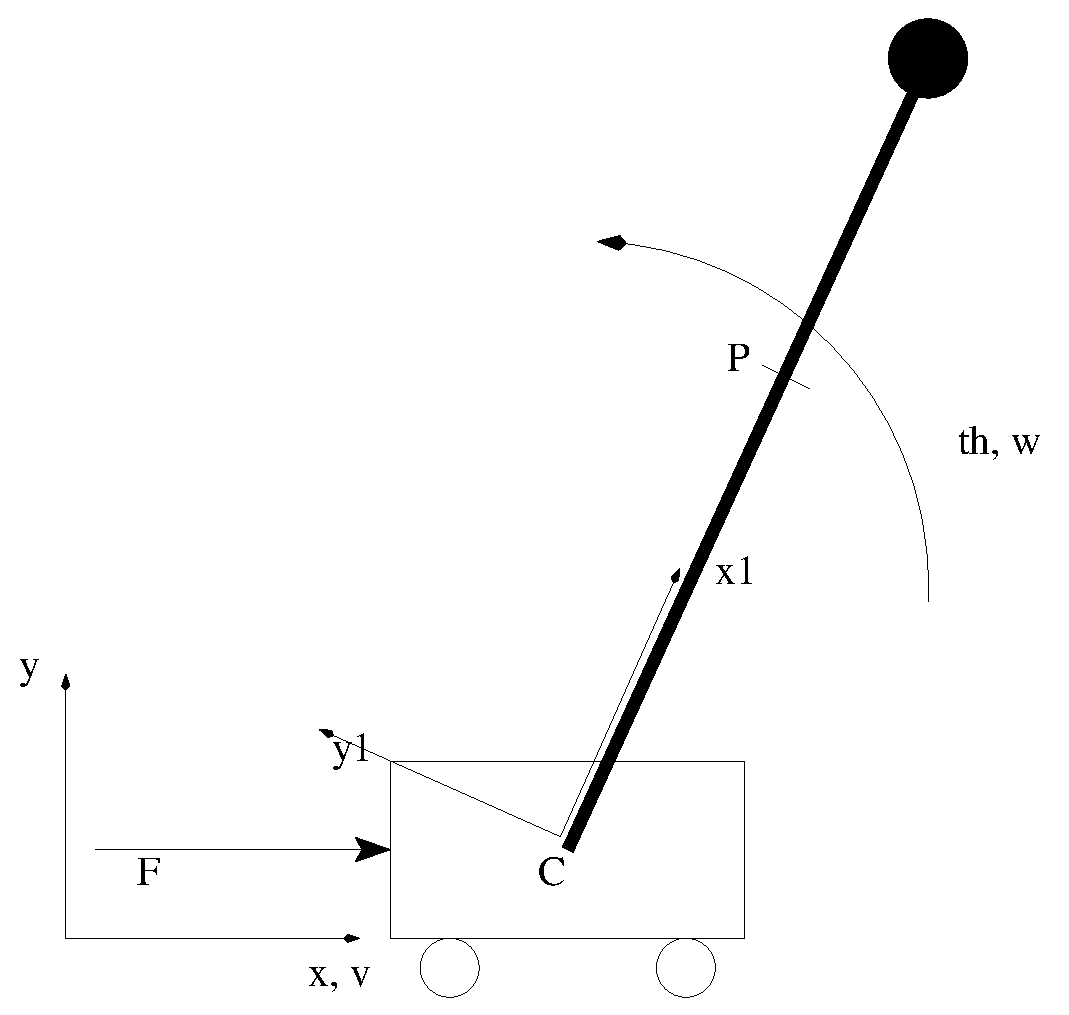
\includegraphics[width=0.55\textwidth]{pendolo.eps}
\caption{Inverted pendulum}
\label{F9a}
\vspace{8mm}
\end{figure}

\begin{figure}[htbp]	% Step
\centering
\vspace{8mm}
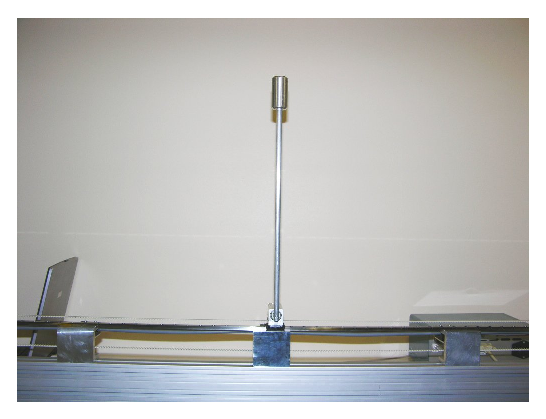
\includegraphics[width=0.55\textwidth]{pendinv.eps}
\caption{Inverted pendulum - Real plant}
\label{F9_a}
\vspace{8mm}
\end{figure}

The global reference frame is \textbf{Nf} ($x$, $y$)
The point \textbf{P} is the center of mass of the pendulum. The car is moving 
with speed \textbf{v} and position \textbf{C}.
The pole is rotating with the angle \textbf{th} and angular velocity 
\textbf{w}, 
In addition to the main coordinate frame \textbf{Nf} ($x$, $y$), we define a 
local body-fixed frame to the pendulum \textbf{Npend} ($x_1$, $y_1$).

\subsection{Modules and constants}
\begin{code}
In [1]: from sympy import symbols, Matrix, pi
   ...: from sympy.physics.mechanics import *
   ...: import numpy as np
   ...: 
   ...: # Modeling the system with Kane method
   ...: 
   ...: # Signals
   ...: x, th  = dynamicsymbols('x th')
   ...: v, w = dynamicsymbols('v w')
   ...: F = dynamicsymbols('F')
  ...: 
   ...: # Constants
   ...: d = symbols('d') # friction
   ...: m, r = symbols('m r')
   ...: M = symbols('M')
   ...: g, t = symbols('g t')
   ...: J = symbols('J')
   ...: 
\end{code}

\subsection{Frames - Car and pendulum}
\begin{code}
In [2]: # Frames and Coord. system
   ...: 
   ...: # Car - reference x,y
   ...: Nf = ReferenceFrame('Nf')
   ...: C = Point('C')                         
   ...: C.set_vel(Nf, v*Nf.x)
   ...: Car = Particle('Car',C,M)
   ...: 
   ...: # Pendulum - reference x1, y1
   ...: Npend = Nf.orientnew('Npend','Axis',[th,Nf.z])
   ...: Npend.set_ang_vel(Nf,w*Nf.z)
   ...: 
   ...: P = C.locatenew('P',r*Npend.x)
   ...: P.v2pt_theory(C,Nf,Npend)
   ...: Pa = Particle('Pa', P, m)
   ...: 
\end{code}

\subsection{Points, bodies, masses and inertias}
\begin{code}
In [3]: I = outer (Nf.z, Nf.z)
   ...: Inertia_tuple = (J*I, P)
   ...: Bp = RigidBody('Bp', P, Npend, m, Inertia_tuple)
   ...: 
\end{code}

\subsection{Forces, frictions and gravity}
\begin{code}
In [4]: # Forces and torques
   ...: forces = [(C,F*Nf.x-d*v*Nf.x),(P,-m*g*Nf.y)]
   ...: frames = [Nf,Npend]
   ...: points = [C,P]
   ...: 
   ...: kindiffs = [x.diff(t)-v, th.diff(t) - w]
   ...: particles = [Car,Bp]
   ...: 
\end{code}

\subsection{Final model and linearized state-space matrices}
\begin{code}
n [5]: # Model
   ...: KM = KanesMethod(Nf,q_ind=[x,th],u_ind=[v,w], kd_eqs=kindiffs)
   ...: fr,frstar = KM.kanes_equations(forces,particles)
   ...: 
   ...: # Equilibrium point
   ...: eq_pt = [0, pi/2,0,0]
   ...: eq_dict = dict(zip([x,th,v,w], eq_pt))
   ...: 
   ...: # symbolically linearize about arbitrary equilibrium
   ...: linear_state_matrix, linear_input_matrix, inputs = 
KM.linearize(new_method=True)
   ...: 
   ...: # sub in the equilibrium point and the parameters
   ...: f_A_lin = linear_state_matrix.subs(eq_dict)
   ...: f_B_lin = linear_input_matrix.subs(eq_dict)
   ...: m_mat = KM.mass_matrix_full.subs(eq_dict)
   ...: 
   ...: # compute A and B
   ...: A = m_mat.inv() * f_A_lin
   ...: B = m_mat.inv() * f_B_lin
   ...: 
\end{code}

\begin{code}
In [6]: A
Out[6]: 
Matrix([
[0,  0,  1, 0],
[0,  0,  0, 1],
[0,   g*m**2*r**2/(J*M + J*m + M*m*r**2), -d*(m**2*r**2/((M + m)*(J*M + J*m 
+ M*m*r**2)) + 1/(M + m)), 0],
[0, g*m*r*(M + m)/(J*M + J*m + M*m*r**2),                               
-d*m*r/(J*M + J*m + M*m*r**2), 0]])
\end{code}

\begin{code}
In [7]: B
Out[7]: 
Matrix([
[                                                       0],
[                                                       0],
[m**2*r**2/((M + m)*(J*M + J*m + M*m*r**2)) + 1/(M + m)],
[                            m*r/(J*M + J*m + M*m*r**2)]])
\end{code}

And the results can be written in a better form as

$$
A=\left[\begin{matrix}0 & 0 & 1 & 0\\0 & 0 & 0 & 1\\0 & \frac{g m^{2} r^{2}}{Jc 
M + Jc m + M m r^{2}} & - \frac{d \left(Jc + m r^{2}\right)}{Jc M + Jc m + M m 
r^{2}} & 0\\0 & \frac{g m r \left(M + m\right)}{Jc M + Jc m + M m r^{2}} & - 
\frac{d m r}{Jc M + Jc m + M m r^{2}} & 0\end{matrix}\right]
$$

and 

$$
B=\left[\begin{matrix}0\\0\\\frac{Jc + m r^{2}}{Jc M + Jc m + M m 
r^{2}}\\\frac{m r}{Jc M + Jc m + M m r^{2}}\end{matrix}\right]
$$

\section{Model of the Ball-on-Wheel plant}

A more complex plant is represented by the Ball-on-Wheel system of 
figure~\ref{F9b}, where a ball must be maintened in the unstable equilibrium 
point on the top of a bike wheel.

\begin{figure}[htbp]	% Step
\centering
% \psfrag{ph0}{$\varphi_0$} 
% \psfrag{ph1}{$\varphi_1$} 
% \psfrag{ph2}{$\varphi_2$} 
% \psfrag{w1}{$\omega_1$} 
% \psfrag{w2}{$\omega_2$} 
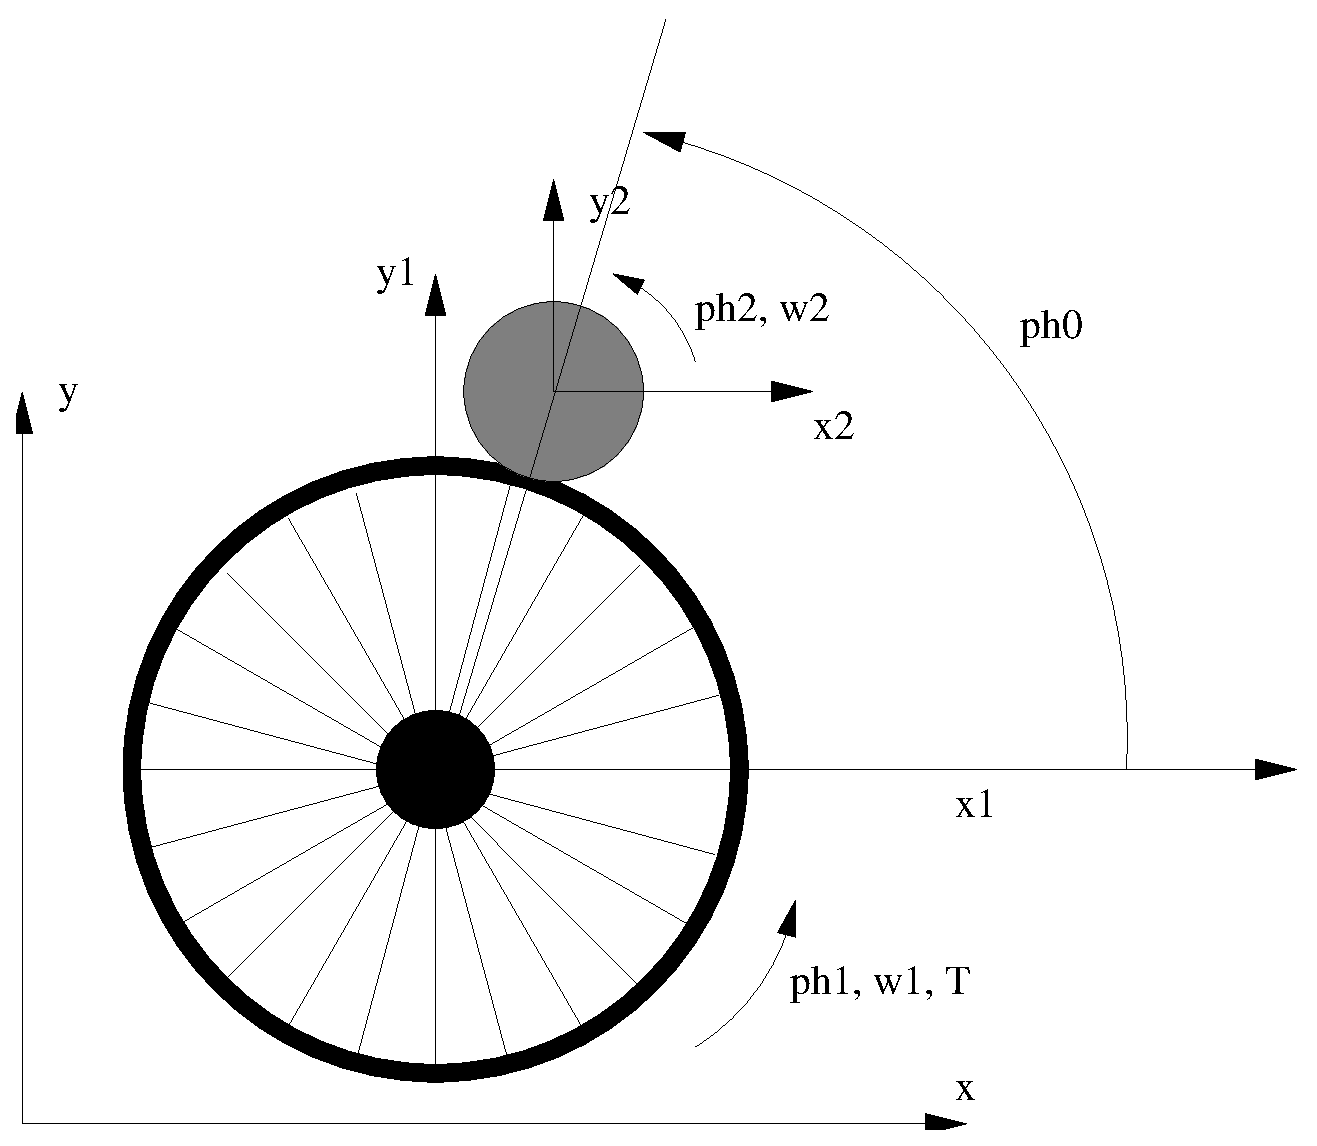
\includegraphics[width=0.5\textwidth]{BallOnWheel.eps}
\caption{Ball-On-Wheel plant}
\label{F9b}
\end{figure}

In this system we have 4 reference frames. The frame \textbf{N} is the main 
reference frame, \textbf{N0} rotates with the line connecting the centers of 
mass of the wheel (\textbf{O}) and of the ball (\textbf{CM2}), \textbf{N1} 
($x_1$, $y_1$) rotates with the wheel and \textbf{N2} ($x_2$, $y_2$) is 
body-fixed to the ball.

The radius of the wheel and of the ball are respectively $R_1$ and $R_2$. The 
non sliding condition is given by

$$
(R_1+R_2) \cdot ph_0=R_1 \cdot ph_1 + R_2 \cdot ph_2
$$

The input of the system is represented by the torque $T$ applied to the wheel.

\subsection{Modules and constants}
\begin{code}
In [1]: from sympy import symbols, Matrix, pi
   ...: from sympy.physics.mechanics import *
   ...: import numpy as np
   ...: 
   ...: ph0, ph1, ph2 = dynamicsymbols('ph0 ph1 ph2')
   ...: w1, w2 = dynamicsymbols('w1 w2')
   ...: 
   ...: T = dynamicsymbols('T')
   ...: 
   ...: J1, J2 = symbols('J1 J2')
   ...: M1, M2 = symbols('M1 M2')
   ...: R1, R2 = symbols('R1 R2')
   ...: d1     = symbols('d1')
   ...: g      = symbols('g')
   ...: t      = symbols('t')
   ...: 
\end{code}

\subsection{Reference frames}
\begin{code}
In [2]: N = ReferenceFrame('N')
   ...: 
   ...: O = Point('O')
   ...: O.set_vel(N,0)
   ...: 
   ...: ph0 = (R1*ph1+R2*ph2)/R1
   ...: 
   ...: N0 = N.orientnew('N0','Axis',[ph0,N.z])
   ...: N1 = N.orientnew('N1','Axis',[ph1,N.z])
   ...: N2 = N.orientnew('N2','Axis',[ph2,N.z])
   ...: N1.set_ang_vel(N,w1*N.z)
   ...: N2.set_ang_vel(N,w2*N.z)
   ...: 

\end{code}

\subsection{Centers of mass of the ball}
\begin{code}
In [3]: CM2 = O.locatenew('CM2',(R1+R2)*N0.y)
   ...: CM2.v2pt_theory(O,N,N0)
   ...: 
Out[3]: (-R1*ph1' - R2*ph2')*N0.x
\end{code}

\subsection{Masses and inertias}
\begin{code}
In [4]: Iz = outer(N.z,N.z)
   ...: In1T = (J1*Iz, O)
   ...: In2T = (J2*Iz, CM2)
   ...: 
   ...: B1 = RigidBody('B1', O, N1, M1, In1T)
   ...: B2 = RigidBody('B2', CM2, N2, M2, In2T)
   ...: 
\end{code}

\subsection{Forces and torques}
\begin{code}
In [5]: #forces = [(N1, (T-d1*w1)*N.z), (CM2,-M2*g*N.y)]
   ...: forces = [(N1, T*N.z), (CM2,-M2*g*N.y)]
   ...: 
   ...: kindiffs = [ph1.diff(t)-w1,ph2.diff(t)-w2]
   ...: 
\end{code}

\subsection{Kane's model and linearized state-space matrices}
\begin{code}
In [6]: KM = KanesMethod(N,q_ind=[ph1, ph2],u_ind=[w1, w2],kd_eqs=kindiffs)
   ...: fr, frstar = KM.kanes_equations(forces,[B1, B2])
   ...: 

In [7]: # Equilibrium point
   ...: eq_pt = [0, 0, 0, 0, 0]
   ...: eq_dict = dict(zip([ph1,ph2,w1,w2, T], eq_pt))
   ...: 

In [8]: # symbolically linearize about arbitrary equilibrium
   ...: linear_state_matrix, linear_input_matrix, inputs = 
KM.linearize(new_method=True)
   ...: 
   ...: # sub in the equilibrium point and the parameters
   ...: f_A_lin = linear_state_matrix.subs(eq_dict)
   ...: f_B_lin = linear_input_matrix.subs(eq_dict)
   ...: m_mat = KM.mass_matrix_full.subs(eq_dict)
   ...: 
   ...: # compute A and B
   ...: A = m_mat.inv() * f_A_lin
   ...: B = m_mat.inv() * f_B_lin
\end{code}

\begin{code}
In [9]: A
Out[9]: 
Matrix([
[0, 0, 1, 0],
[0, 0, 0, 1],
[-M2**2*R1**2*R2**2*g/((R1 + R2)*(J1*J2 + J1*M2*R2**2 + J2*M2*R1**2)) + 
M2*R1**2*g*(M2**2*R1**2*R2**2/((J1 + M2*R1**2)*(J1*J2 + J1*M2*R2**2 + 
J2*M2*R1**2)) + 1/(J1 + M2*R1**2))/(R1 + R2), -M2**2*R1*R2**3*g/((R1 + 
R2)*(J1*J2 + J1*M2*R2**2 + J2*M2*R1**2)) + M2*R1*R2*g*(M2**2*R1**2*R2**2/((J1 + 
M2*R1**2)*(J1*J2 + J1*M2*R2**2 + J2*M2*R1**2)) + 1/(J1 + M2*R1**2))/(R1 + R2), 
0, 0],
[                                           -M2**2*R1**3*R2*g/((R1 + R2)*(J1*J2 
+ J1*M2*R2**2 + J2*M2*R1**2)) + M2*R1*R2*g*(J1 + M2*R1**2)/((R1 + R2)*(J1*J2 + 
J1*M2*R2**2 + J2*M2*R1**2)),                                      
-M2**2*R1**2*R2**2*g/((R1 + R2)*(J1*J2 + J1*M2*R2**2 + J2*M2*R1**2)) + 
M2*R2**2*g*(J1 + M2*R1**2)/((R1 + R2)*(J1*J2 + J1*M2*R2**2 + J2*M2*R1**2)), 0, 
0]])
In [10]: B
Out[10]: 
Matrix([
[                                                                               
           0],
[                                                                               
           0],
[M2**2*R1**2*R2**2/((J1 + M2*R1**2)*(J1*J2 + J1*M2*R2**2 + J2*M2*R1**2)) + 
1/(J1 + M2*R1**2)],
[                                              -M2*R1*R2/(J1*J2 + J1*M2*R2**2 + 
J2*M2*R1**2)]])
\end{code}

or as formula

$$
A=\left[\begin{smallmatrix}0 & 0 & 1 & 0\\0 & 0 & 0 & 1\\\frac{J_{2} M_{2} 
R_{1}^{2} g}{J_{1} J_{2} R_{1} + J_{1} J_{2} R_{2} + J_{1} M_{2} R_{1} 
R_{2}^{2} + J_{1} M_{2} R_{2}^{3} + J_{2} M_{2} R_{1}^{3} + J_{2} M_{2} 
R_{1}^{2} R_{2}} & \frac{J_{2} M_{2} R_{1} R_{2} g}{J_{1} J_{2} R_{1} + J_{1} 
J_{2} R_{2} + J_{1} M_{2} R_{1} R_{2}^{2} + J_{1} M_{2} R_{2}^{3} + J_{2} M_{2} 
R_{1}^{3} + J_{2} M_{2} R_{1}^{2} R_{2}} & 0 & 0\\\frac{J_{1} M_{2} R_{1} R_{2} 
g}{\left(R_{1} + R_{2}\right) \left(J_{1} J_{2} + J_{1} M_{2} R_{2}^{2} + J_{2} 
M_{2} R_{1}^{2}\right)} & \frac{J_{1} M_{2} R_{2}^{2} g}{\left(R_{1} + 
R_{2}\right) \left(J_{1} J_{2} + J_{1} M_{2} R_{2}^{2} + J_{2} M_{2} 
R_{1}^{2}\right)} & 0 & 0\end{smallmatrix}\right]
$$

and

$$
B=\left[\begin{smallmatrix}0\\0\\\frac{M_{2}^{2} R_{1}^{2} 
R_{2}^{2}}{\left(J_{1} + M_{2} R_{1}^{2}\right) \left(J_{1} J_{2} + J_{1} M_{2} 
R_{2}^{2} + J_{2} M_{2} R_{1}^{2}\right)} + \frac{1}{J_{1} + M_{2} 
R_{1}^{2}}\\- \frac{M_{2} R_{1} R_{2}}{J_{1} J_{2} + J_{1} M_{2} R_{2}^{2} + 
J_{2} M_{2} R_{1}^{2}}\end{smallmatrix}\right]
$$

\chapter{Control design}

\section{PI+Lead design example}

\subsection{Define the system and the project specifications}

In this first example we design a controller for a plant with the transfer 
function
 
$$
G(s)=\frac{1}{s^2 + 6\cdot s + 5}
$$
 
The requirements for the control are
 
$$
e_{\infty} = 0
$$ 
 
for a step input
 
$$
PM\geq60^o
$$
 
and
 
$$
\omega_{gc} = 10rad/s
$$

The controller can be written in the form

$$
C(s) = K \cdot \frac{1+s \cdot T_i}{s \cdot T_i} \cdot \frac{1+\alpha \cdot T_D 
\cdot s}{1+ s \cdot T_D}
$$

with a PI and a lead part.

We have to design the controller and find the values of $\mathbf{T_i}$, 
$\mathbf{\alpha}$, 
$\mathbf{T_D}$ and $\mathbf{K}$. The full design is performed using the bode 
diagram.

After installing the required modules, we can define the plant transfer 
function and the requirements of the project.
 
\begin{code}
In [1]: # Modules

In [2]: from matplotlib.pyplot import *

In [3]: from control import *

In [4]: from numpy import pi, linspace

In [5]: from scipy import sin, sqrt

In [6]: from supsisim.RCPblk import *

In [7]: from supsictrl.ctrl_utils import *

In [8]: from supsictrl.ctrl_repl import *

In [9]: g=tf([1],[1,6,5])

In [10]: bode(g,dB=True);

In [11]: legend(['G(s)'],prop={'size':10})
Out[11]: 
(<matplotlib.axes.AxesSubplot at 0x7f85b5193550>,
 <matplotlib.legend.Legend at 0x7f85b47e6950>)

In [12]: wgc = 10         # Desired Bandwidth

In [13]: desiredPM = 60   # Desired Phase margin
\end{code}

Figure~\ref{F10} shows the bode diagram of the plant.

\begin{figure}[htbp]	% Step
\centering
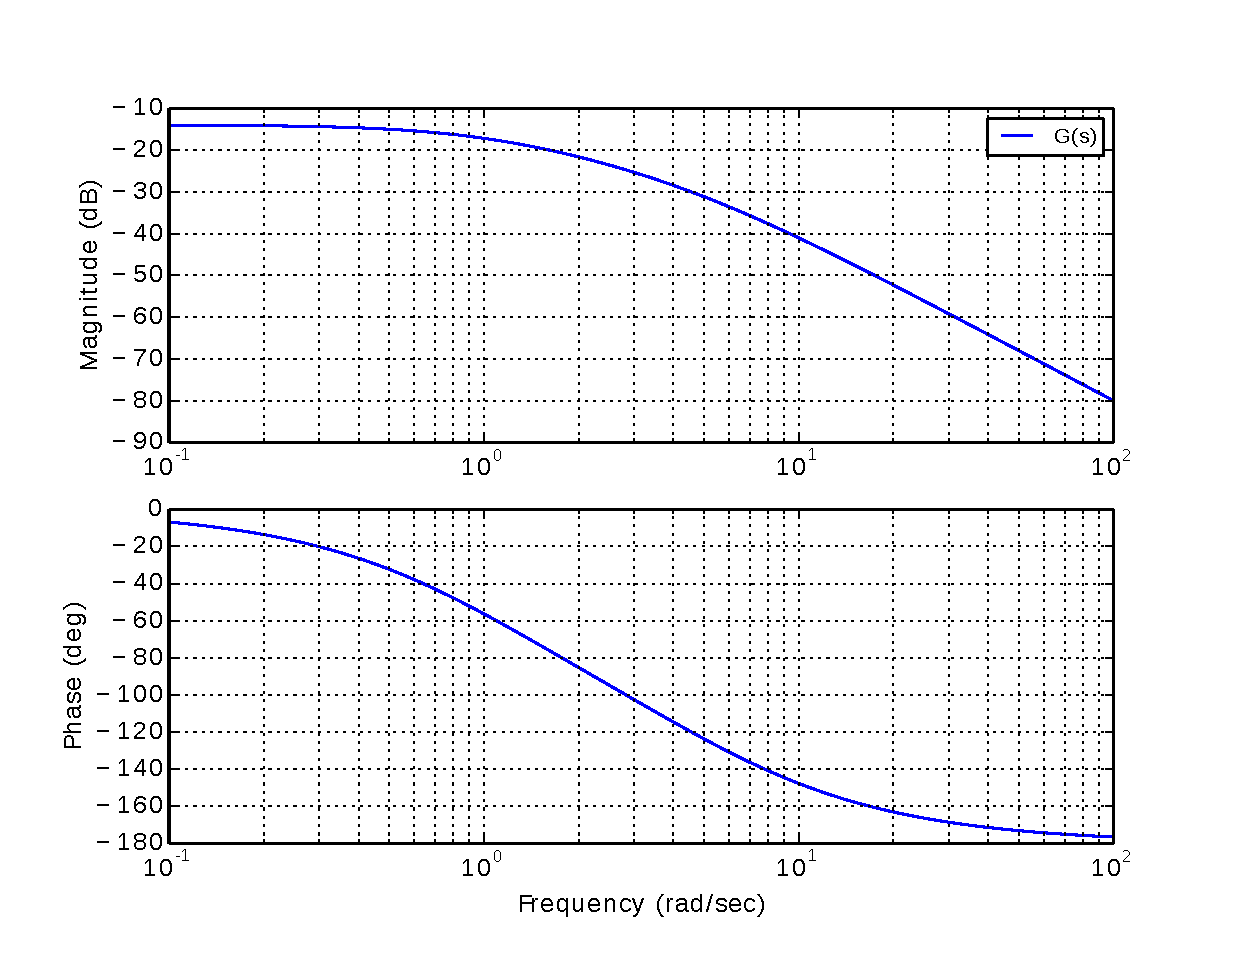
\includegraphics[width=0.6\textwidth]{eps/bodeplant.eps}
\caption{Bode diagram of the plant}
\label{F10}
\end{figure}

\subsection{PI part}

Now we choose the integration time for the PI part of the controller. In this 
example we set

$$
T_i=0.15s
$$

\begin{code}
In [14]: # PI part

In [15]: Ti=0.15

In [16]: Gpi=tf([Ti,1],[Ti,0])

In [17: print "PI part is: ", Gpi
PI part is:  
0.15 s + 1
----------
  0.15 s


In [18: figure()
Out[18: <matplotlib.figure.Figure at 0x7f85b47eaa10>

In [19: bode(g,dB=True,linestyle='dashed');

In [20 hold
Out[20 <function matplotlib.pyplot.hold>

In [21 bode(Gpi*g,dB=True);

In [22: legend((['G(s)','Gpi(s)*G(s)']),prop={'size':10})
Out[22: 
(<matplotlib.axes.AxesSubplot at 0x7f85b4806250>,
 <matplotlib.legend.Legend at 0x7f85b4303850>)
\end{code}

Figure~\ref{F11} shows the bode plot of the plant with and without the PI 
controller part.

\begin{figure}[htbp]	% Step
\centering
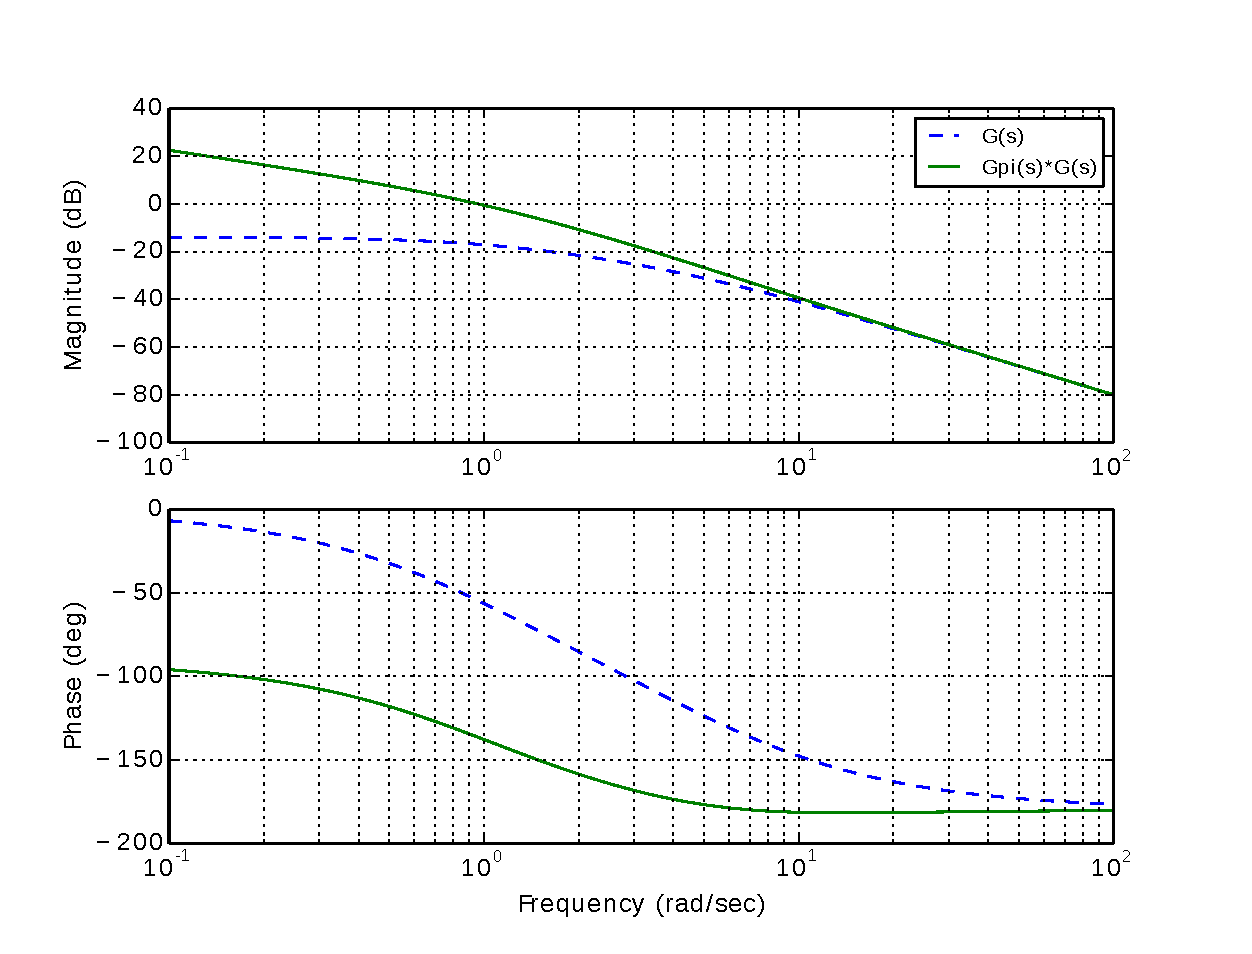
\includegraphics[width=0.7\textwidth]{eps/bodeplantpi.eps}
\caption{Bode diagram: G (dashed) and Gpi*G}
\label{F11}
\end{figure}

\subsection{Lead part}

Now we can get the $PM$ at the frequency $\omega_{gc}$ in order to calculate 
the additional phase contribution of the lead part of the controller.

\begin{code}
In [23: mag,phase,omega = bode(Gpi*g,[wgc],Plot=False)

In [24: ph = phase[0]

In [25: if ph>=0:
    ...:     ph = phase[0]-360;
    ...:     

In [26: Phase = -180+desiredPM

In [27: dPM = Phase-ph

In [28: print "Additional phase from Lead part: ", dPM
Additional phase from Lead part:  61.4144232114
\end{code}

Now it is possible to calculate the lead controller by finding the values of 
$\alpha$ and $T_D$.

\begin{code}
In [29]: # Lead part

In [30]: dPMrad = dPM/180*pi

In [31]: alfa = (1+sin(dPMrad))/(1-sin(dPMrad));

In [32]: print "Alpha is: ", alfa
Alpha is:  15.4073552425

In [33]: TD = 1/(sqrt(alfa)*wgc);

In [34]: Glead = tf([alfa*TD,1],[TD,1])

In [35]: print "Lead part is: ", Glead
Lead part is:  
 0.3925 s + 1
-------------
0.02548 s + 1


In [36]: figure()
Out[36]: <matplotlib.figure.Figure at 0x7f85b43462d0>

In [37]: bode(g,dB=True,linestyle='dashed');

In [38]: hold
Out[38]: <function matplotlib.pyplot.hold>

In [39]: bode(Gpi*Glead*g, dB=True);

In [40]: 
legend((['G(s)','Gpi(s)*G(s)','Gpi(s)*GLead(s)*G(s)']),prop={'size':10})
Out[40]: 
(<matplotlib.axes.AxesSubplot at 0x7f85b43736d0>,
 <matplotlib.legend.Legend at 0x7f85b3b1f450>)
\end{code}

Figure~\ref{F12} shows now the bode plot of the plant, the plant with the PI 
part and the plant with PI and Lead part

\begin{figure}[htbp]	% Step
\centering
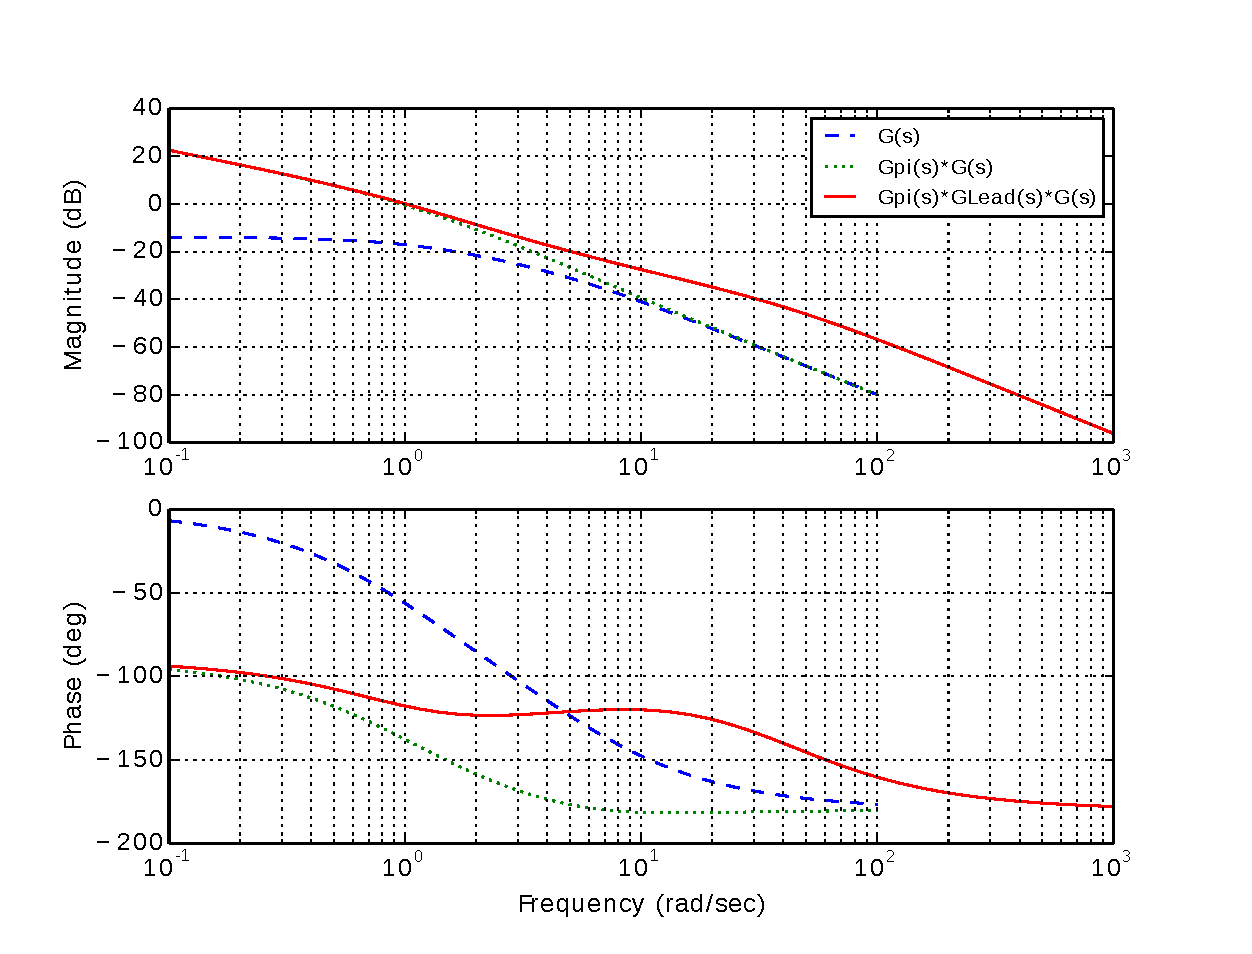
\includegraphics[width=0.6\textwidth]{eps/bodeplantpilead.eps}
\caption{Bode diagram - G (dashed), Gpi*G (dotted) and Gpi*GLead*G}
\label{F12}
\end{figure}

\subsection{Controller Gain}

The last step is to find the amplification $K$ of the controller which move up 
the bode gain plot in order to obtain the required crossover frequency 
$\omega_{gc}$.

\begin{code}
In [41]: mag,phase,omega = bode(Gpi*Glead*g,[wgc],Plot=False)

In [42]: print "Phase at wgc is: ", phase[0]
Phase at wgc is:  -120.0

In [43]: K=1/mag[0]

In [44]: print "Gain to have MAG at gwc 0dB: ", K
Gain to have MAG at gwc 0dB:  23.8177769548

In [45]: figure()
Out[45]: <matplotlib.figure.Figure at 0x7f85b3a703d0>

In [46]: bode(g,dB=True,linestyle='dashed');

In [47]: hold
Out[47]: <function matplotlib.pyplot.hold>

In [48]: bode(Gpi*Glead*g, dB=True,linestyle='-.');

In [49]: bode(K*Gpi*Glead*g, dB=True);

In [50]: 
legend((['G(s)','Gpi(s)*G(s)','Gpi(s)*GLead(s)*G(s)',
'K*Gpi(s)*GLead(s)*G(s)']),prop={'size':10})
Out[50]: 
(<matplotlib.axes.AxesSubplot at 0x7f85b3a76690>,
 <matplotlib.legend.Legend at 0x7f85b33e6f90>)
\end{code}

In the figure~\ref{F13} we see now that the gain plot has been translated up to 
get $0dB$ at the gain crossover frequency $\omega_{gc}$.

\begin{figure}[htbp]	% Step
\centering
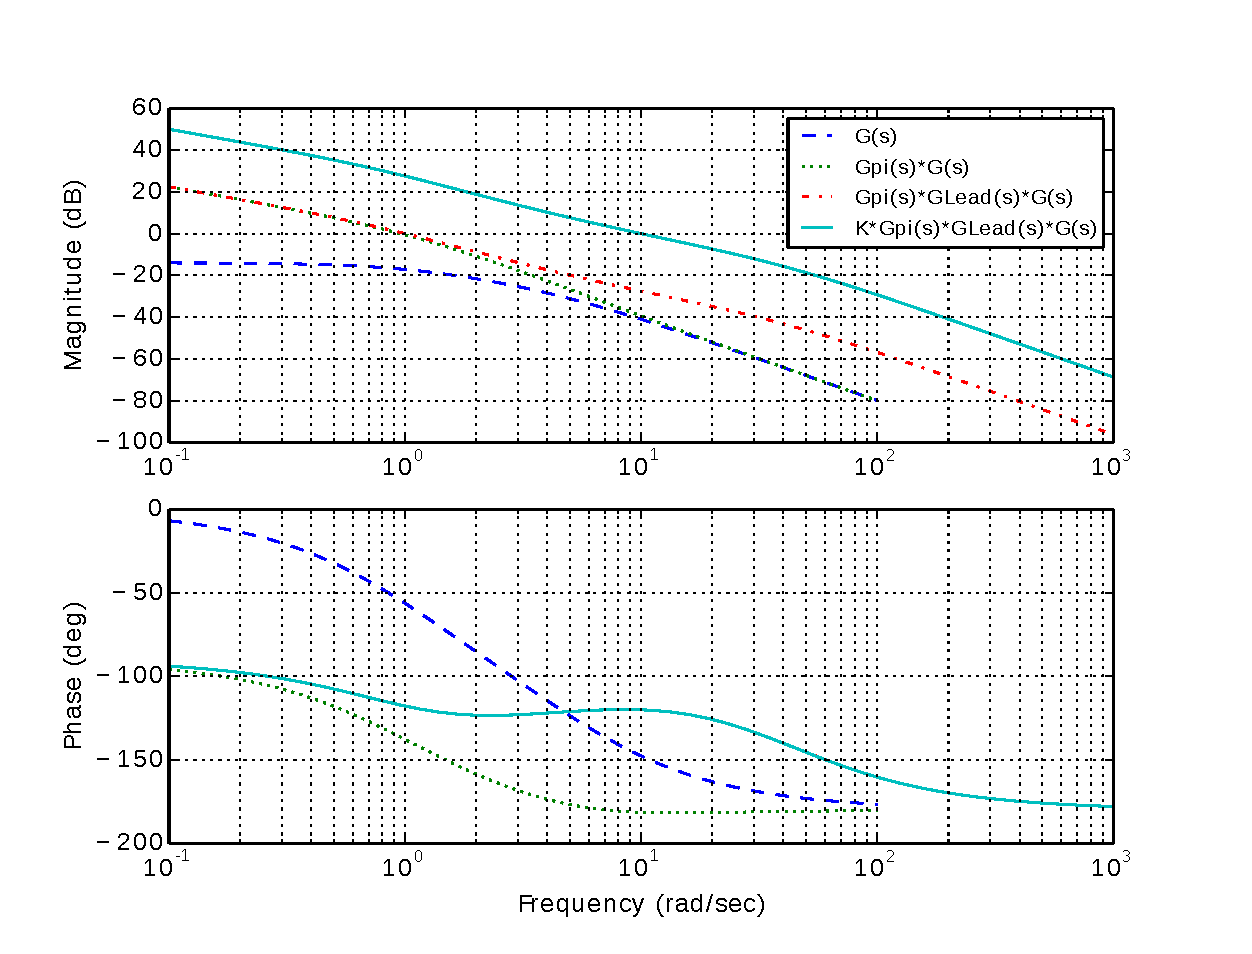
\includegraphics[width=0.6\textwidth]{eps/bodeplantpileadK.eps}
\caption{Bode diagram - G (dashed), Gpi*G (dotted), Gpi*GLead*G (dot-dashed) 
and K*Gpi*GLead*G}
\label{F13}
\end{figure}

\subsection{Simulation of the controlled system}

Now it is possible to simulate the controlled system after closing the loop.

\begin{code}
In [51]: Contr = K*Gpi*Glead

In [52]: print "Full controller: ", Contr
Full controller:  
1.402 s^2 + 12.92 s + 23.82
---------------------------
   0.003821 s^2 + 0.15 s

In [53]: mag,phase,omega = bode(K*Gpi*Glead*g,[wgc],Plot=False)

In [54]: print "Data at wgc - wgc: ", omega[0], "Magnitude: ",mag[0], "Phase: 
",phase[0]
Data at wgc - wgc:  10 Magnitude:  1.0 Phase:  -120.0

In [55]: gt=feedback(K*Gpi*Glead*g,1)

In [56]: t=linspace(0,1.5,300)

In [57]: y,t = step(gt,t)

In [58]: figure()
Out[58]: <matplotlib.figure.Figure at 0x7f85b3514290>

In [59]: plot(t,y), xlabel('t'), ylabel('y'), title('Step response of the 
controlled plant')
Out[59]: 
([<matplotlib.lines.Line2D at 0x7f85b34252d0>],

In [60]: grid()
\end{code}

The simulation of the controlled plant with a step input is shown in 
figure~\ref{F14}.

\begin{figure}[htbp]	% Step
\centering
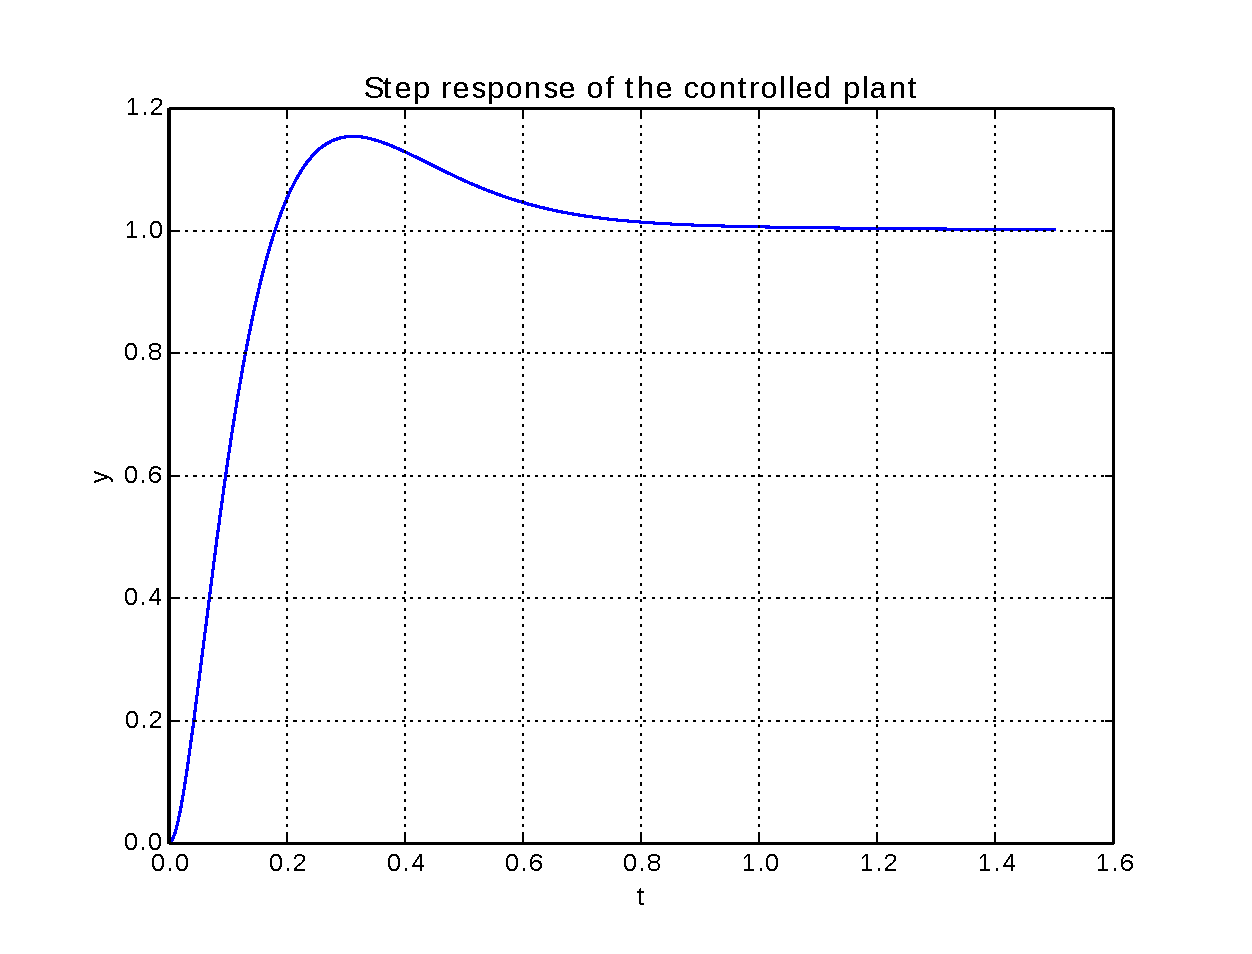
\includegraphics[width=0.7\textwidth]{eps/pidexastep.eps}
\caption{Step response of the controlled plant}
\label{F14}
\end{figure}

\section{Discrete-state feedback controller design}

\subsection{Plant and project specifications}

In this example we design a discrete-state feedback controller for a DC servo 
motor. 

We want to have a controlled system with a maximum of $4\%$ 
overshooting and an error $e_{\infty}=0$ with a step input. In addition we 
desire a bandwidth of the controlled system of at least $6$ rad/s.

The step response of the motor with the current input of $I_{in}=500mA$) has 
been saved into the file ``MOT''.

\subsection{Motor parameters identification}

We try to find the parameters of the srvo motor using a least square 
identification from the collected data.

The transfer function of the DC motor from input current $I(s)$ to output angle 
$\Phi(s)$ can be represented as

$$
G(s)=\frac{\Phi(s)}{I_{in}(s)}=\frac{K_t/J}{s^2 + s \cdot D/J}
$$

\subsection{Required modules}

\begin{code}
In [1]: from scipy.optimize import leastsq

In [2]: from scipy.signal import step2

In [3]: import numpy as np

In [4]: import scipy as sp

In [5]: from control import *

In [6]: from control.Matlab import *

In [7]: from supsisim.RCPblk import *
   ...: from supsictrl.ctrl_utils import *
   ...: from supsictrl.ctrl_repl import *
   ...: 

\end{code}

\subsection{Function for least square identification}
We define now the function \textbf{residuals} which returns the error between 
the collected and the simulated data. 
Using this function we can try to minimize the error using a least square 
approach.

\begin{code}
In [8]: # Motor response for least square identification

In [9]: def residuals(p, y, t):  
   ...:     [k,alpha] = p
   ...:     g = tf(k,[1,alpha,0])
   ...:     Y,T = step(g,t)
   ...:     err=y-Y
   ...:     return err
   ...: 
\end{code}

\subsection{Parameter identification}
We load the collected data to perform the parameter identification of the 
numerator $K=K_t/J$ and the  denominator value $\alpha=D/J$.

\begin{code}
In [10]: # Identify motor

In [11]: x = np.loadtxt('MOT');

In [12]: t = x[:,0]

In [13]: y = x[:,2] 

In [14]: Io = 1000

In [15]: y1 = y/Io

In [16]: p0 = [1,4]

In [17]: plsq = leastsq(residuals, p0, args=(y1, t))

In [18]: kt = 0.0000382          # Motor torque constant

In [19]: Jm=kt/plsq[0][0]        # Motor Inertia

In [20]: Dm=plsq[0][1]*Jm        # Motor friction

In [21]: g=tf([kt/Jm],[1,Dm/Jm,0])  # Transfer function
\end{code}

\subsection{Check of the identified parameters}

The next step is to check how good our parameters have been identified by 
comparing the simulated function with the measured data (see figure~\ref{F15})

\begin{code}
In [22]: Y,T = step(g,t)

In [23]: plot(T,Y,t,y1), legend(('Identified transfer function','Collected 
data'),prop={'size':10},loc=2), xlabel('t'), ylabel('y'), title('Step 
response'), grid()
Out[23]: 
([<matplotlib.lines.Line2D at 0x7fb9a1b6b590>,
  <matplotlib.lines.Line2D at 0x7fb9a1b6b710>],
 <matplotlib.legend.Legend at 0x7fb9a1b6bb10>,
 <matplotlib.text.Text at 0x7fb9a3cec310>,
 <matplotlib.text.Text at 0x7fb9a1b8b910>,
 <matplotlib.text.Text at 0x7fb9a1b3cbd0>,
 None)
\end{code}

\begin{figure}[htbp]	% Step
\centering
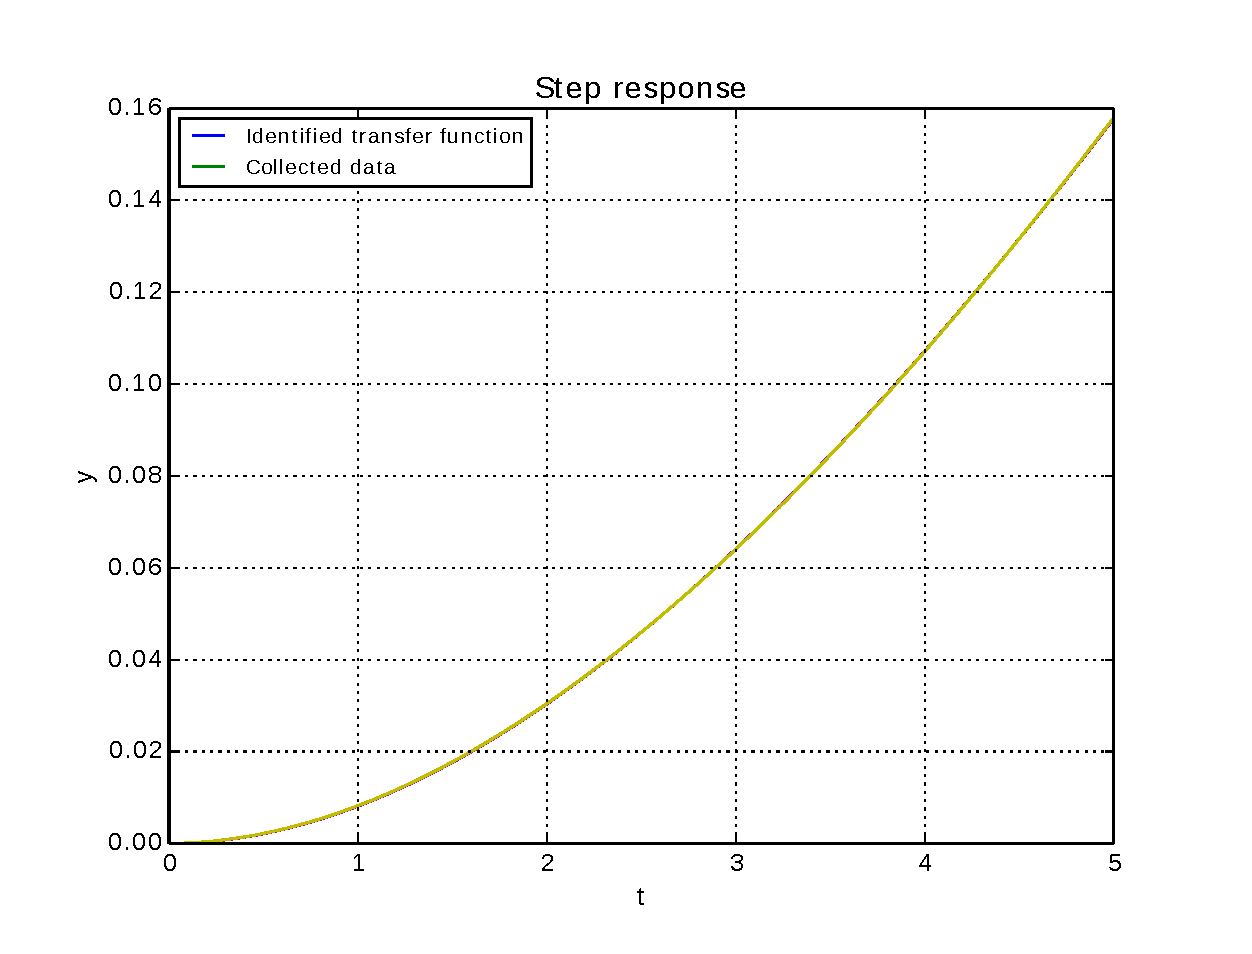
\includegraphics[width=0.8\textwidth]{eps/motid.eps}
\caption{Step response and collected data}
\label{F15}
\end{figure}

\subsection{Continuous and discrete model}
For the state controller design we need to model our motor in the state-space 
form. We define the continuous-state and the discrete-state space model

\begin{code}
In [24]: # Design Controller Motor 1

In [25]: a=[[0,1],[0,-Dm/Jm]]

In [26]: b=[[0],[1]]

In [27]: c=[[kt/Jm,0]];

In [28]: d=[0];

In [29]: sysc=ss(a,b,c,d)                # Continuous state-space form

In [30]: Ts=0.01                         # Sampling time

In [31]: sys = c2d(sysc,Ts,'zoh')        # Discrete ss form
\end{code}

\subsection{Controller design}
For the controller we set a bandwidth to $6$ rad/s with a damping factor of
$\xi=\sqrt{2}/2$.

\begin{code}

In [32]: # Control system design

In [33]: print rank(ctrb(sys.A,sys.B))==2    # Controllability check
True

In [34]: # State feedback with integral part

In [35]: wn=6

In [36]: xi=np.sqrt(2)/2

In [37]: angle = np.arccos(xi)
\end{code}

We add a discrete integral part to eliminate the steady state error and we 
obtain an additional state for the error between reference and output signal. 
The two matrices $\Phi$ and $\Gamma$ required by the pole placement routine 
must be extended with the additional state.

\begin{code}

In [38]: cl_poles = -wn*array([1, exp(1j*angle), exp(-1j*angle)] ) # three poles

In [39]: cl_polesd=sp.exp(cl_poles*Ts)    # Desired discrete poles

In [40]: sz1=sp.shape(sys.A);

In [41]: sz2=sp.shape(sys.B);

In [42]: # Add discrete integrator for steady state zero error

In [43]: Phi_f=np.vstack((sys.A,-sys.C*Ts))

In [44]: Phi_f=np.hstack((Phi_f,[[0],[0],[1]]))

In [45]: G_f=np.vstack((sys.B,zeros((1,1))))

In [46]: k=place(Phi_f,G_f,cl_polesd)
\end{code}

\subsection{Observer design}

Now we can implement the observer: in this example we choose a reduced-order 
observer and we can use the function provided by the yottalab module to obtain
it.

\begin{code}
In [47]: #Reduced order observer

In [48]: print rank(obsv(sys.A,sys.C))==2     # Observability check
True

In [49]: p_oc=-10*max(abs(cl_poles))

In [50]: p_od=sp.exp(p_oc*Ts);

In [51]: T=[0,1]

In [52]: r_obs=red_obs(sys,T,[p_od])
\end{code}

\subsection{Controller in compact form}

The yottalab function \textbf{comp\_form\_i} allows to integrate the controller 
gains and the observer into an unique block.

\begin{code}
In [53]: # Controller + integral + observer in compact form

In [54]: contr_I=comp_form_i(sys,r_obs,k)
\end{code}

\subsection{Anti windup}

The last operation consists in  dividing the controller into an input part and 
a feedback 
part in order to realize the anti-windup mechanism and considering the 
saturation block.

\begin{code}
In [55]: # Anti windup

In [56]: [gss_in, gss_out]=set_aw(contr_I,[0,0])
\end{code}

\subsection{Simulation of the controlled plant}

The block diagram of the final controlled system is represented in 
figure~\ref{F16}.

\begin{figure}[htbp]	% Step
\centering
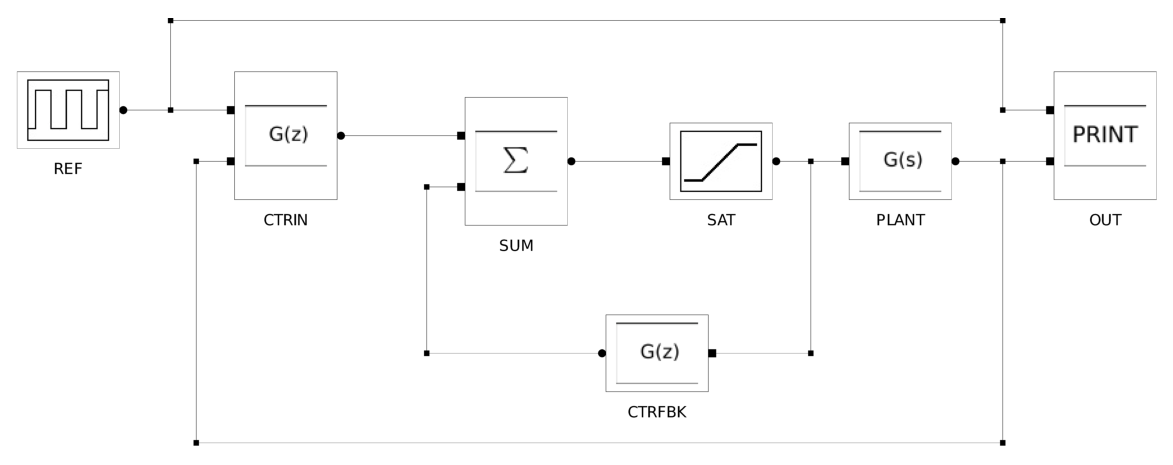
\includegraphics[width=0.8\textwidth]{ctrmot.eps}
\caption{Block diagram of the controlled system}
\label{F16}
\end{figure}

It is not possible to simulate the resulting system in Python because of:

\begin{itemize}
\item The controller is discrete and the plant is continuous. At present it is 
not possible to perform hybrid simulation usin the control package. In some 
cases we can substitute the plant with the discrete-time system and perform a 
discrete 
simulation. Hybrid simulation is possible using the pyEdit application 
described in the next chapter.
\item The block ``CTRIN'' has two inputs. The step function can only find the 
output from a single input.
\item The control toolbox can handle only linear system (and there is a 
saturation in the final system).
\end{itemize}

\chapter{Hybrid simulation and code generation}

\section{Basics}

CACSD environments usually offer a graphical 
editor to perform the hybrid simulation (Matlab$\leftrightarrow$Simulink, 
Scioslab$\leftrightarrow$Scicos, Scilab$\leftrightarrow$xCos etc.).

The ``pyEdit.py'' application should cover this task for the Python Control 
environment.

In the following we'll explain how it is possible, from the pyEdit schematics, 
to generate code for the hybrid simulation. Code for the RT controller can be 
generated in the same way: users should only replace the mathematical model 
of the plant with the blocks interfacing the sensors and the actuators of the 
real system.

\section{pyEdit}

\subsection{The editor}

The application ``pyEdit`` is a block diagram editor to design schematics for 
simulation and code generation.

Starting points for the pyEdit application were the PySimEd project 
(\cite{PSE}) and the qtnodes-develop project (\cite{QTNODES}).

PyEdit offers the most used blocks in control design. A little set of these 
blocks is shown in figure~\ref{F17}.
 
 \begin{figure}[htbp]	% Step
 \centering
 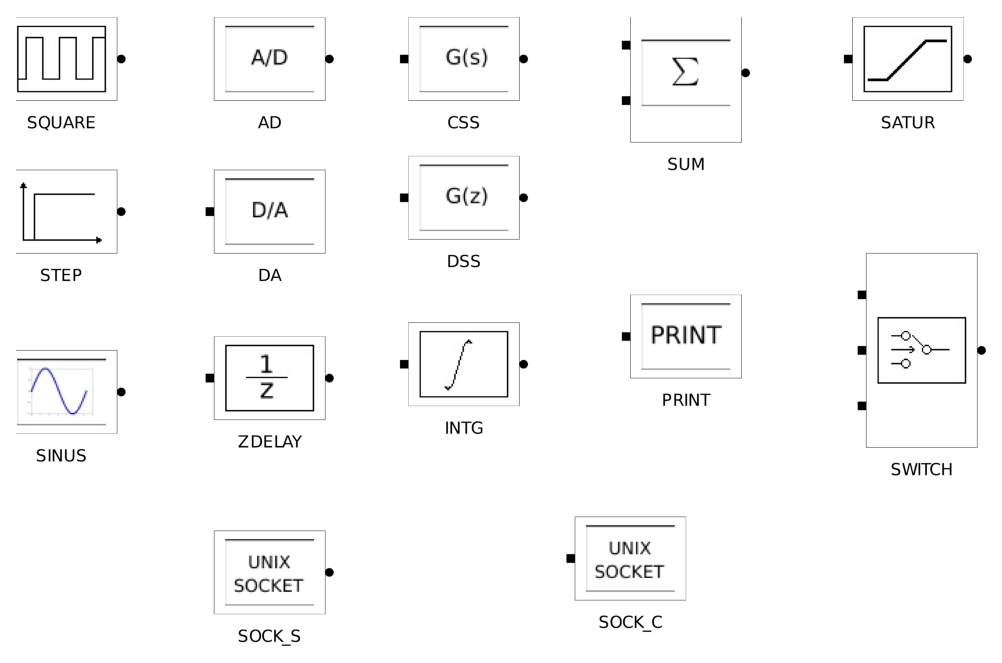
\includegraphics[width=0.7\textwidth]{blocks.eps}
 \caption{Some pyEdit blocks for control design}
 \label{F17}
 \end{figure}
 
 \subsection{The first example}
 Using the editor we wont create the block diagram of figure~\ref{Fig:exa1}.
 
\begin{figure}[htbp]	% Step
\centering
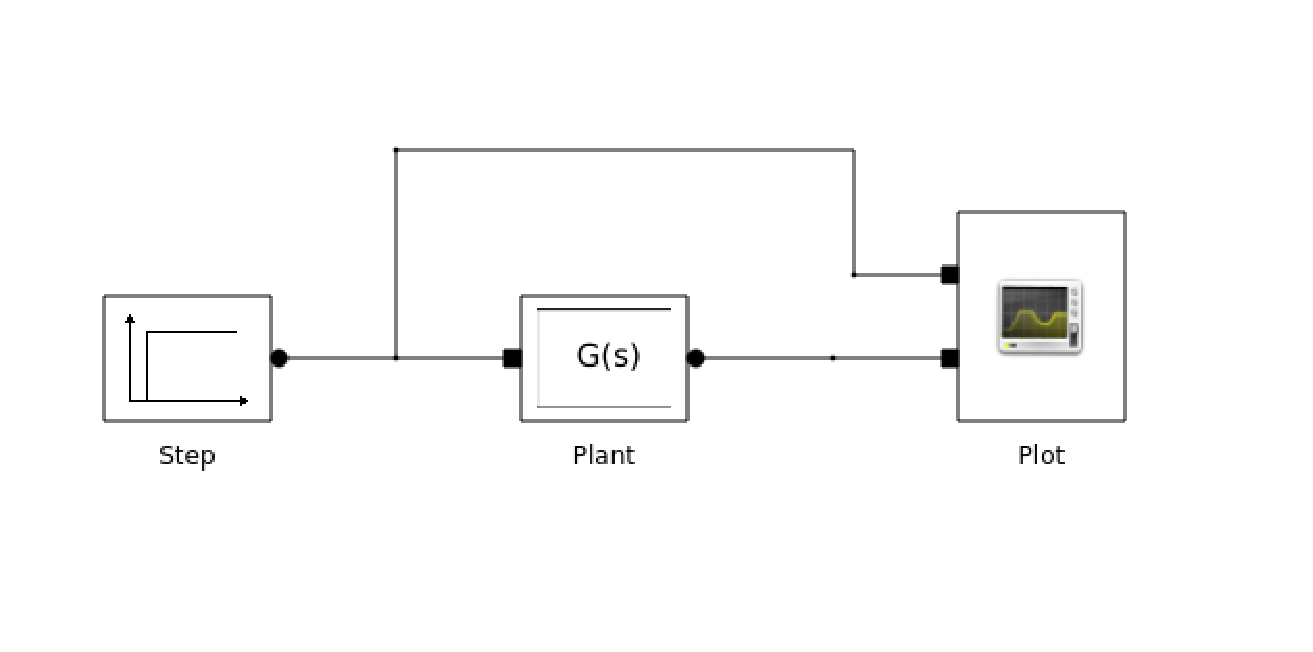
\includegraphics[width=0.7\textwidth]{exa_final.eps}
\caption{The first example}
\label{Fig:exa1}
\end{figure}

We open a shell and we give the command
 
\begin{verbatim}
pyEdit
\end{verbatim}

The application opens 2 windows as shown in figure~\ref{Fig:envEdit}

\begin{figure}[htbp]	% Step
\centering
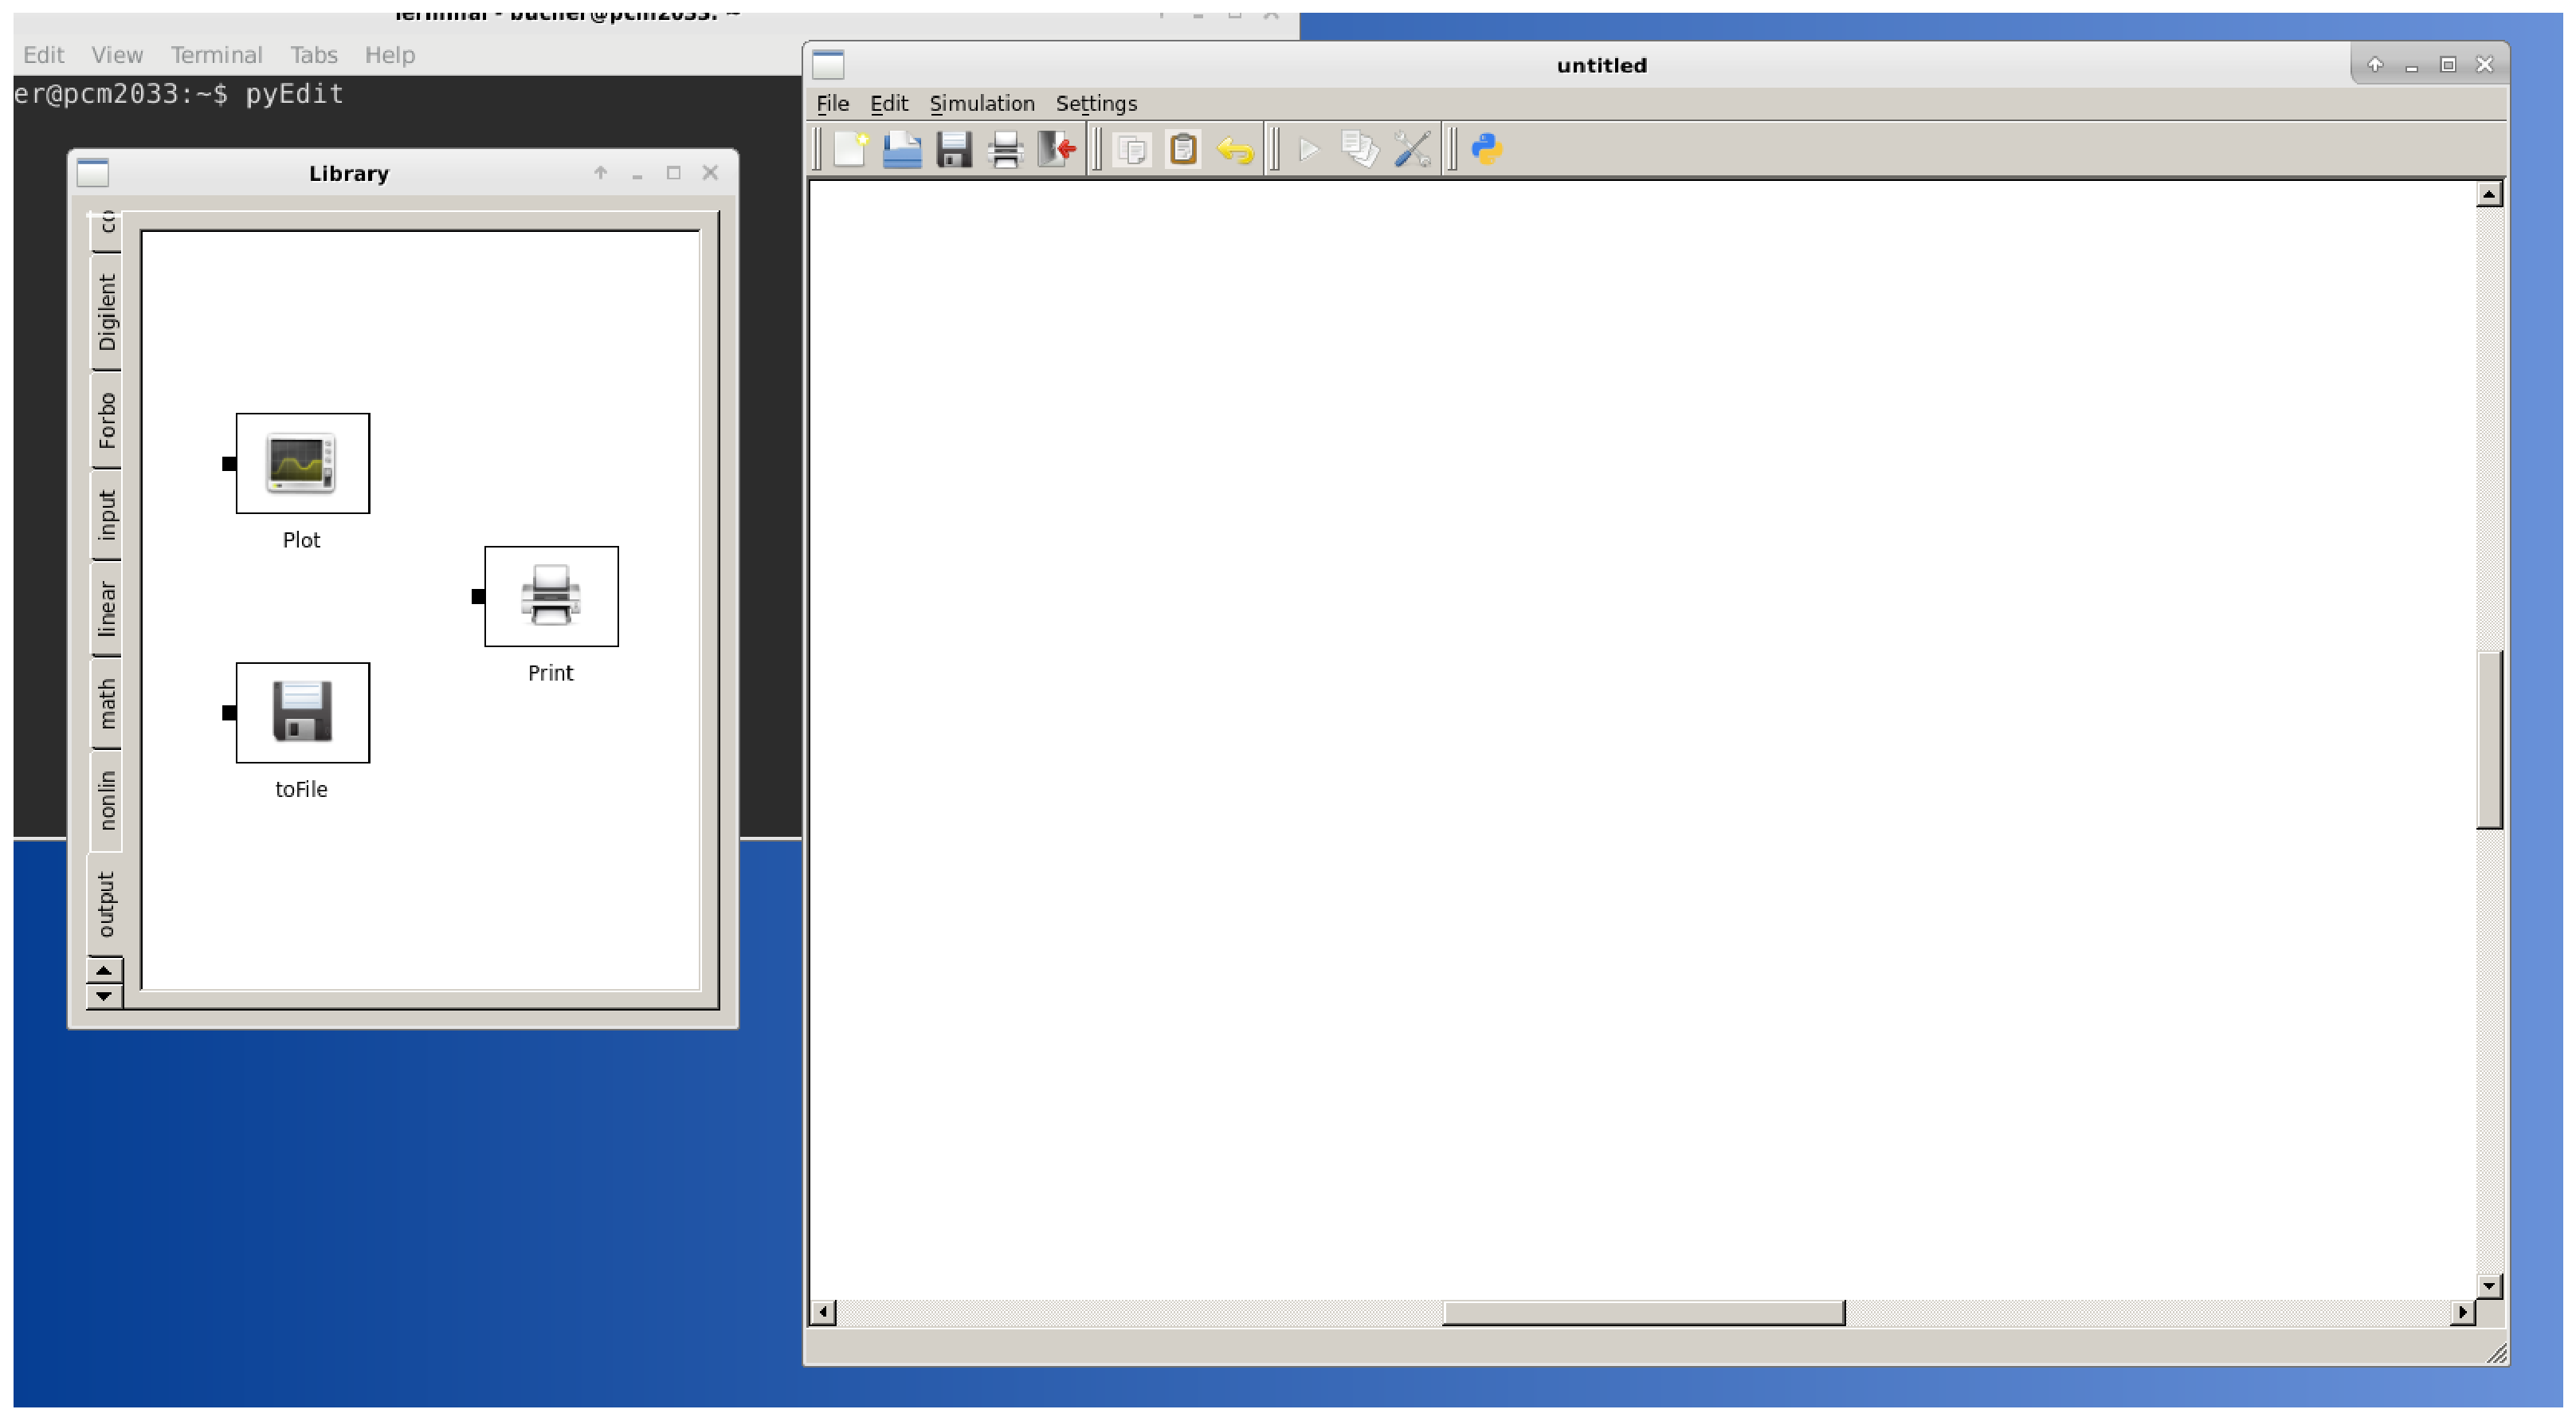
\includegraphics[width=\textwidth]{env_pyEdit.eps}
\caption{The pyEdit environment}
\label{Fig:envEdit}
\end{figure}

The window on the left shows the library with the available blocks and on the 
right we have the diagram window. Now we can start to draw our block diagram.

From the library window we can choos the tab ''input`` and using ''drag and 
drop`` we can get the block ''Step`` and move it into the editor window. We can 
do the same operation with the ''LTI continous`` (from tab ''linear``) and the 
''Plot`` (from tab ''output``) blocks.

Now we should obtain the diagram shown in figure~\ref{Fig:exa_step1}

\begin{figure}[htbp]	% Step
\centering
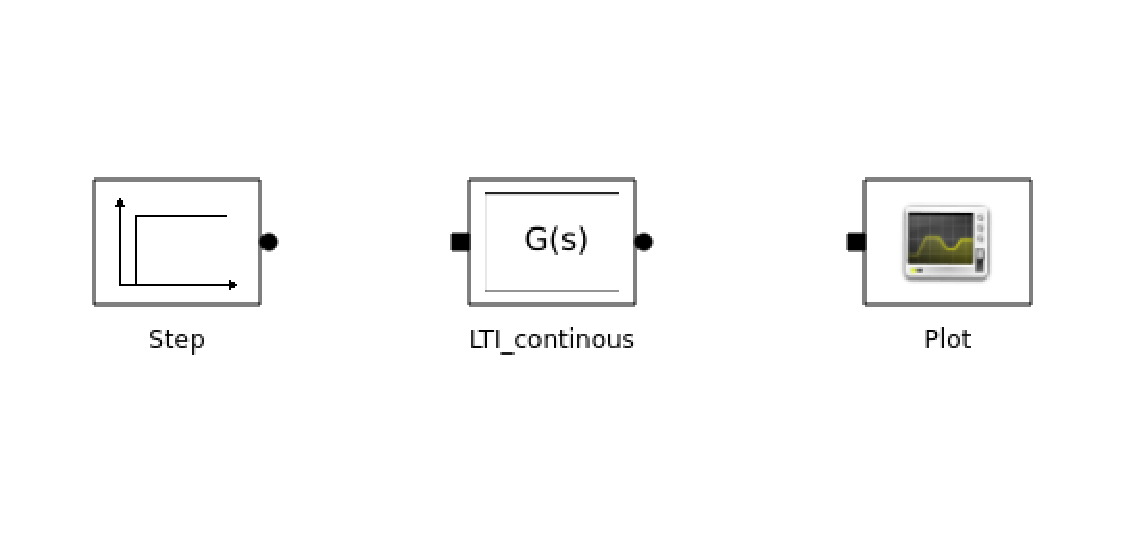
\includegraphics[width=0.7\textwidth]{exa_step1.eps}
\caption{Result from the drag and drop operations}
\label{Fig:exa_step1}
\end{figure}

Before starting with the connection, we set some parameters to the blocks.

\begin{itemize}
\item Souble click with the mouse on the block ''LTI continous``. In the dialog 
windows set the System to \textbf{tf(1,[1,1])}
\item Click the right mouse on the LTI continous block``. In the new menu 
choose ''Change Name`` and rename it as \textbf{Plant}.
\item Click the right mouse on the Plot block. In the new menu choose ``Block 
I/Os'' and set the number of inputs to \textbf{2}.
\end{itemize}

Figure~\ref{Fig:exa_step2} shows the new diagram.

\begin{figure}[htbp]	% Step
\centering
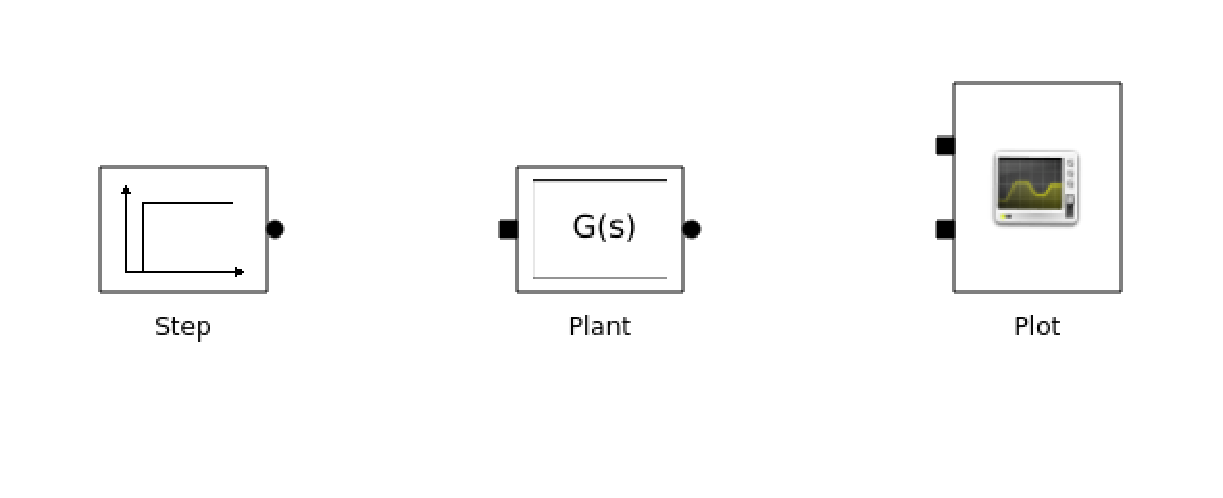
\includegraphics[width=0.7\textwidth]{exa_step2.eps}
\caption{Result after parametrization}
\label{Fig:exa_step2}
\end{figure}

Now we can proceed with the connections.

\begin{itemize}
\item Move the mouse on the output of the block ``Step'': the mouse pointer 
should become a ``cross''. Click and release the left mouse button.
\item Now we can move the mouse to the input of the block ``Plant'': the mouse 
pointer should become a ``cross''. Click and release the left mouse button.
\item Do the same operation from the output of the block ``Plant'' to the 
second input of the block ``Plot''
\item Now move to the node (the little circle) between the ``Step'' and the 
block ``Plant'': the mouse 
pointer should become a ``cross''. Click and release the left mouse button.
\item move the mouse up, click, and continue to move left the mouse. Left of 
the position of the block ``Plot'', click and release again the left mouse 
button and then finish the connection on the first input of the block ``Plot'' 
(click and release the left mouse button)
\end{itemize}

You should obtain the diagram of figure~\ref{Fig:exa1}

Now we are able to simulate the diagram.

\begin{itemize}
\item From the menu ``Simulation'' choose ``Simulate'' or click on the button 
``Simulate'' on the toolbar (the button with the triangle).
\item Double click with the mouse on the block ``Plot'' to get the graphical 
output of the simulation (see figure~\ref{Fig:exaplot}).
\end{itemize}

\begin{figure}[htbp]	% Step
\centering
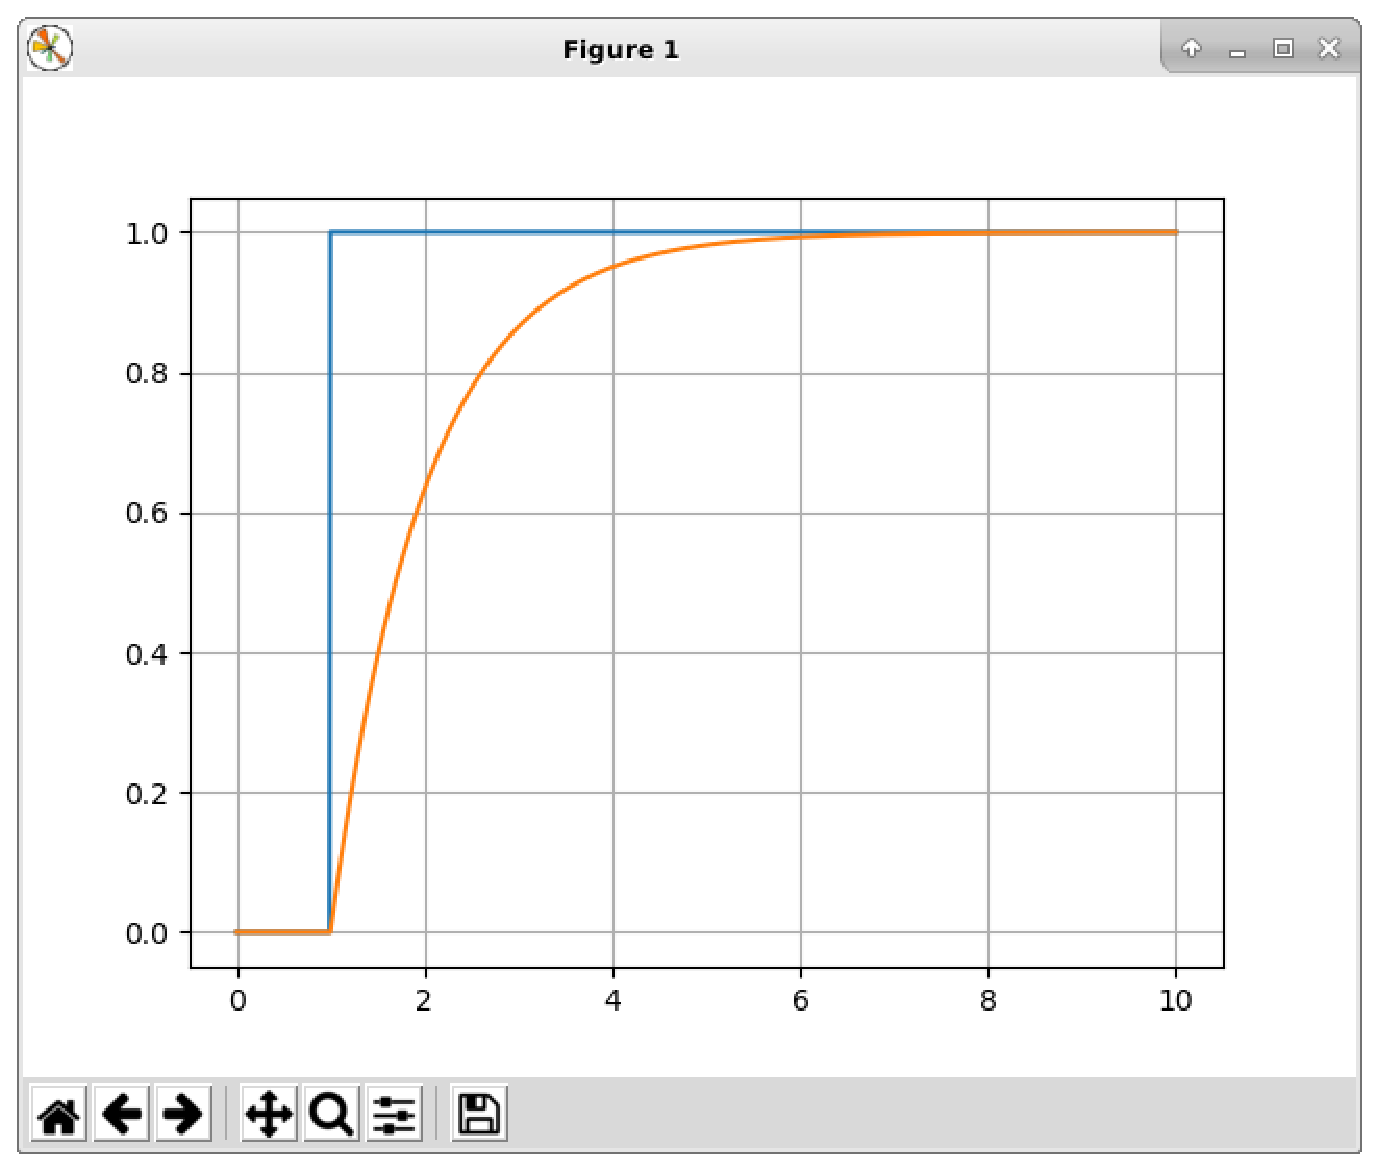
\includegraphics[width=0.4\textwidth]{exa_plot.eps}
\caption{Result (plot) of the simulation}
\label{Fig:exaplot}
\end{figure}

\subsection{Personalize the most used blocks}
A special file ``common.blks'' is defined in the ``resources/block/block'' 
folder. This file contains a list of clocks, that the user can modify to have 
its own most used blocks. The blocks are shown in the library both in the 
``common'' tab and in the specific tab.

\subsection{Defining new blocks}
The user can define new blocks and integrate them into the pyEdit application.

First of all he have to define the ``.xblk'' file, using for example the 
application ``defBlock'' (which is part of pycontrol.tgz). This block must be 
moved in the folder ``~/Documents/PYTHON/blocks''.

A new function must be inserted in the file ``~/Document/PYTHON/userBlocks.py'' 
(the file must be created the first time that the user insert a new block!). 
\textbf{The first line of this file must be}:

\begin{code}
from supsisim.RCPblk import RCPblk
\end{code}

Then, the user must define a function for each new block. In the following there 
are some example with 3 blocks, the first with only input ports, the second with 
only output ports, and the last with both input and output ports.

\begin{code}
from supsisim.RCPblk import RCPblk

def digilent_AOBlk(pin, ch):
    if np.size(pin) != 1:
        raise ValueError("Block should have 1 input port; received %i !" % 
np.size(pin))

    blk = RCPblk('digilent_analog_output',pin,[],[0,0],0,[],[ch])
    return blk

def digilent_AIBlk(pout, ch, rng, offset):
    if np.size(pout) != 1:
        raise ValueError("Block should have 1 input port; received %i !" % 
np.size(pout))

    blk = RCPblk('digilent_analog_input',[],pout,[0,0],0,[rng, offset],[ch])
    return blk

def MeanFilterBlk(pin, pout, N):
    blk = RCPblk('meanfilter',pin,pout,[0,0],1,[],[N,0])
    return blk

\end{code}

The implementation of the RCPblk class is defined in the file 
``toolbox/supsisim/src/RCPblk.py''.

\subsection{Some remarks}
\begin{itemize}
\item the simulation result (Plot) \textbf{is available only after the 
simulation}. Please be sure to restart the simulation before opening the plot 
result. The simualtion creates a file with the name of the block in ``/tmp'' 
folder: this file is overwritten by every new simulation.
\item For the simulation, the application creates and compile a C-executable. 
The sources are written in the folder ``xxxxxx\_gen'', where ``xxxxx'' is the 
name of the diagram.
\end{itemize}


\section{The editor window}

\subsection{The toolbar}

The application offers  set of operations in the toolbar as shown in the 
figure~\ref{Fig:pyEdit}.

\begin{figure}[htbp]
 \centering
 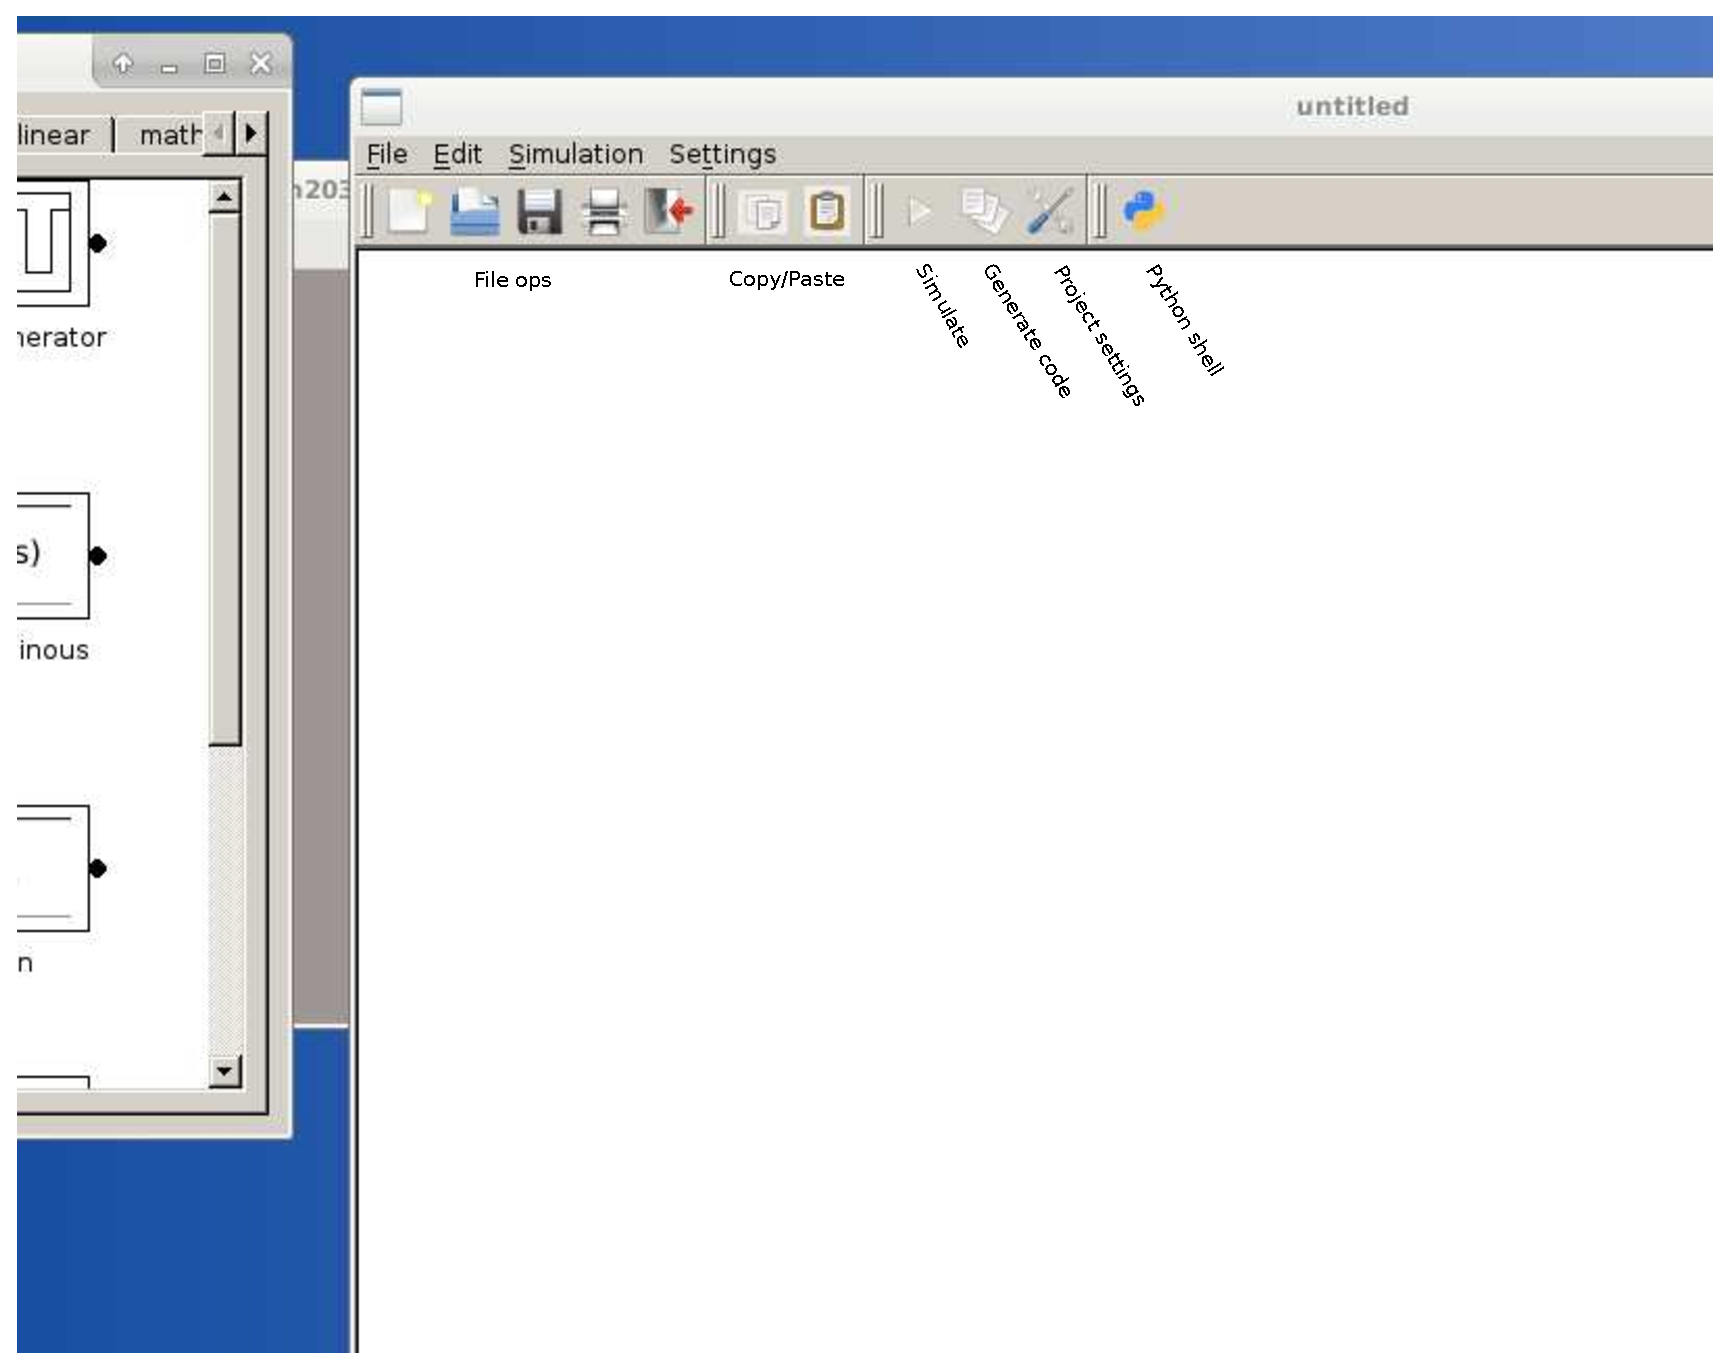
\includegraphics[width=0.8\textwidth]{pyedit.eps}
 \caption{The pyEdit application}
 \label{Fig:pyEdit}
 \end{figure}

\subsection{Operations with the right mouse button}
Depending on the position of the mouse, clicking and releasing the right mouse 
button leads to different behaviours.

\subsection{Operations with the right mouse button on a block}

Clicking with the right mouse button on a block opens a popup menu with the 
following commands:

\begin{description}
\item [Block I/Os] to modify (if possible) the number of input and output ports 
of the block
\item [Flip block] Flip left/right the block
\item [Change name] Each block in the diagram must have \textbf{a unique name}
\item [Block parameters] to modify the parameters: this operation is available 
with a double click tool
\item [Clone block] to get a copy of the selected block
\end{description}

\subsection{Operations with the right mouse button on a connection}

Moving the mouse on a connection, change the pointer to a pointing hand and by 
clicking with the right mouse button a popup menu is opened with the following 
commands:

\begin{description}
\item[Delete conncetion] deletes the pointed connection
\item [Insert node] inserts a new node on the connection. This is needed for 
examples if we have to draw a new connection.
\end{description}

\subsection{Operations with the right mouse button on a node}

Moving the mouse on a node, change the pointer to a cross and by 
clicking with the right mouse button a popup menu is opened with the following 
commands:

\begin{description}
\item[Delete node] deletes the node and the connections associated with this 
node.
\item [Bind node] eliminate the node without eliminate the connection.
\end{description}

\subsection{Behaviour of the right mouse button by drawing a connection}
Clicking the right mouse button by drawing a connection, put a new node in the 
mouse position and exit the drawing mode.

\section{Basic editor operations}

\subsection{Inserting a block}
Get a block from a library and drag it into the main window.

\subsection{Connecting blocks}
\begin{itemize}
\item Move to the output port of a block or to a node.
\item Click and release the left button of the mouse.
\item Move the mouse to draw the connection.
\item Click again the left mouse on an input port of a block to finish the 
connection or click the mouse to obtain a ''node`` and to continue to draw the 
connection.
\end{itemize}

\subsection{Inserting a node}
\begin{itemize}
\item Move to a connection and click the right mouse button
\item Select the ''insert node`` menu.
\end{itemize}

If a new ''node`` is needed into a connection simply click on it with the right 
mouse button.

\subsection{Deleting a block or a node}
\begin{itemize}
\item Move to a block or node and click with the right mouse button.
\item Choose the submenu ''delete``
\end{itemize}

\section{Remove a node}
\begin{itemize}
\item Move to the node.
\item Click with the right mouse button on the node. 
\item Choose the submenu ''Bind node`` The connection is maintained 
but the node is cleared.
\end{itemize}

\chapter{Simulation and Code generation}

Each element of a block diagram is defined with three or four functions:

\begin{description}
\item [The interface function] that describes how the block must be drawn in 
the block diagram
\item [The Implementation function] that contains the code  to be executed to 
perform the tasks related with this block.
\item The translation of the block into the RCPblk class described in the 
RCPblk.py module
\item A dlg function to implement a special dialog box for the block parameters 
(only if required)
\end{description}

In addition we need to know all the nodes connected to the inputs and to the 
outputs of each block.

\section{Interface functions}

Each block is defined into a file with extension ``.xblk'', stored in 
the ``resources/blocks/blocks'' folder.
The file is defined as a Python dictionary:

\scriptsize
\begin{verbatim}
{"lib": "math", "name": "Sum", "ip": 2, "op": 1, "st": 1, "icon": "SUM", "params": "sumBlk|Gains: [1,-1]"}
\end{verbatim}
\normalsize

using the following fields:

\begin{description}
\item[``lib''] the name of the tab for the block library (example 
``tab'':``linear'')
\item [``name''] the default name of the block
\item [``ip''] number of inputs
\item [``op''] number of outputs
\item [``st''] flag which indicates if the number of I/O can be modified
\item [``icon'']the name of the ``.svg'' file with the icon of the block
\item [``param''] the parameters of the block
\end{description}

The first string in the param field is used as name of the Python function used 
to prepare the block to be translated into C-Code.

The block libraries are loaded after launching the pyEdit application as shown 
in figure~\ref{Fig:app1}

 \begin{figure}[htbp]	% Step
 \centering
 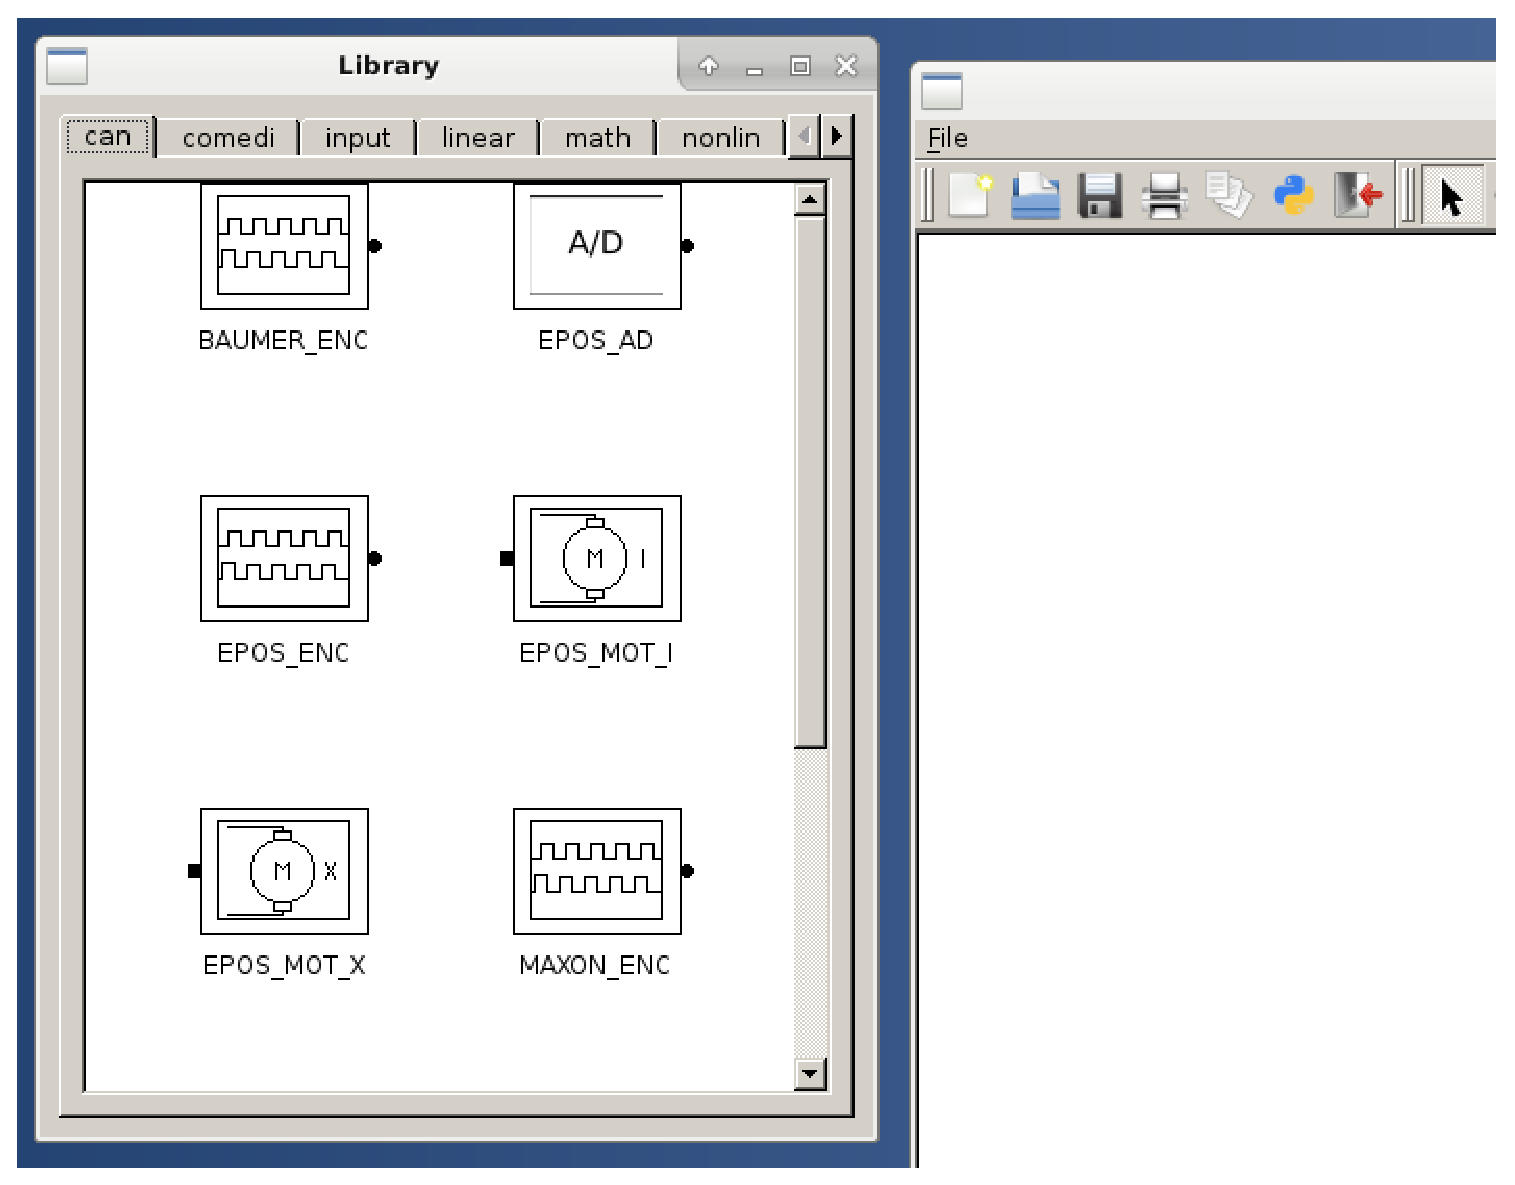
\includegraphics[width=0.9\textwidth]{libs.eps}
 \caption{Window with the block libraries}
 \label{Fig:app1}
 \end{figure}

Each block must be renamed with a unique name (popup menu ``Change name''), and 
its parameters can be modified directly in the pyEdit application with a double 
click.

\section{The implementation functions}

In a schematic, each block can be described with the functions 
(\ref{eq:syscont}) for continuous-time systems or (\ref{eq:sysdisc}) for 
discrete-time systems.

\begin{equation}
\label{eq:syscont}
\begin{array}{lll}
\mathbf{y} & = & \mathbf{g}(\mathbf{x},\mathbf{u},t) \\
\dot{\mathbf{x}} & = & \mathbf{f}(\mathbf{x},\mathbf{u},t) 
\end{array}
\end{equation}

\begin{equation}
\label{eq:sysdisc}
\begin{array}{lll}
\mathbf{y}_k & = & \mathbf{g}(\mathbf{x}_k,\mathbf{u}_k,k) \\
\mathbf{x}_{k+1} & = & \mathbf{f}(\mathbf{x}_k,\mathbf{u}_k,k) 
\end{array}
\end{equation}

The $\mathbf{g}(\ldots)$ function represents the static part of the block. 
This function is used to read inputs, read sensors, write actuators or 
update the outputs of the block.

The second function ($\mathbf{f}(\ldots)$) is only required if the block has 
internal states, and it is only used by dynamic systems. In 
addition, each block implements two other functions, one for the block 
initialization and one to cleanly terminate it.

All these functions are programmed as C-files, compiled and archived into a 
library.

\section{Translating the block into the RCPblk class}
Before generating the C-Code, each block in the diagram must be translated into 
an element of the RCPblk class (see section ~\ref{Sect-IO} for more details).
For each block, the corresponding function (the name is given by the 1. string 
in the parameters line) 
must exists and should be declared with the required parameters. This function 
is responsible to fill all the RCPblk fields.

\section{Special dialog box for the block parameters}
Usually, the graphic editor build a simple dialog box to enter the block 
parameters. 

In special cases, it is possible to write a special function to 
enter the parameters.. In this case, the user should provide this function in 
the RCPDlg.py file.
The name of this function is built using the first string of the parameter 
line, by subsistuting the las 3 letters ``Blk'' with ``Dlg''. This new function 
must receive as input:

\begin{itemize}
\item Numper of inputs
\item Number of outputs
\item The parameters line
\end{itemize}

This function returns a modified parameters line. Anexample is the ``PlotDlg'' 
function in the file ``toolbox/supsisim/src/RCPGDlg.py''.

\section{Example}
We can show with an example what happens with a block in the different phases 
from block to RCPblk class.

The ``Pulse generator'' input block is stored in the ``PulseGenerator.xblk'' 
file with 
the following infos

\tiny
\begin{verbatim}
{"lib": "input", "name": "PulseGenerator", "ip": 0, "op": 1, "st": 0, "icon": 
"SQUARE", "params": "squareBlk|Amplitude: 1|Period: 4|Width: 2|Bias: 0|Delay: 
0"}
\end{verbatim}
\normalsize

The block has no inputs, 1 ouput, the I/O are not modifiable (settable=0).

After a double click on the block, the ``params'' field is parsed and 
translated 
into the the dialog box shown in figure~\ref{Fig:squareblk}.

 \begin{figure}[htbp]	
 \centering
 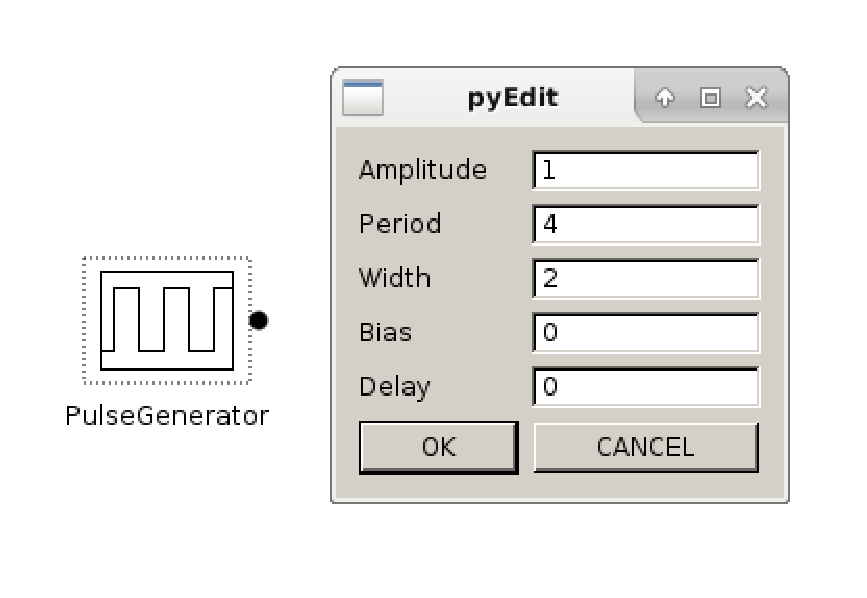
\includegraphics[width=0.6\textwidth]{squareblk.eps}
 \caption{Dialog box for the Pulse generator block}
 \label{Fig:squareblk}
 \end{figure}

 By generating the element of the class RCPblk, the function ``squareBlk'' is 
called with the following parameters:
 
 \begin{verbatim}
 SQUARE = squareBlk(pout, Amp, Period, Width, Bias, Delay)
 \end{verbatim}
 
 where
 
 \begin{description}
 \item[pout] is the matrix with the id of the inputs (connections)
 \item [Amp] is the signal amplitude
 \item [Period] is the period of the signal
 \item [width] is the duration where the signal has value ``Amp-bias''
 \item [bias] is an offset for the signal
 \item [delay] represent the time wenn the signal start
 \end{description}
 
 The function translate the block into the following object of the RCPblk class
 
 \begin{verbatim}
 Function           : square
Input ports        : []
Output ports      : [2]
Nr. of states      : [0 0]
Relation u->y      : 0
Real parameters    : [ 4  8  3  0 12]
Integer parameters : []
\end{verbatim}

\section{The parameters for the code generation}

Before clicking on the ``code generation'' tool on the toolbar, the user should 
fill some parameters in a dialog box (see figure~\ref{codedlg}).

 \begin{figure}[htbp]	% Step
 \centering
 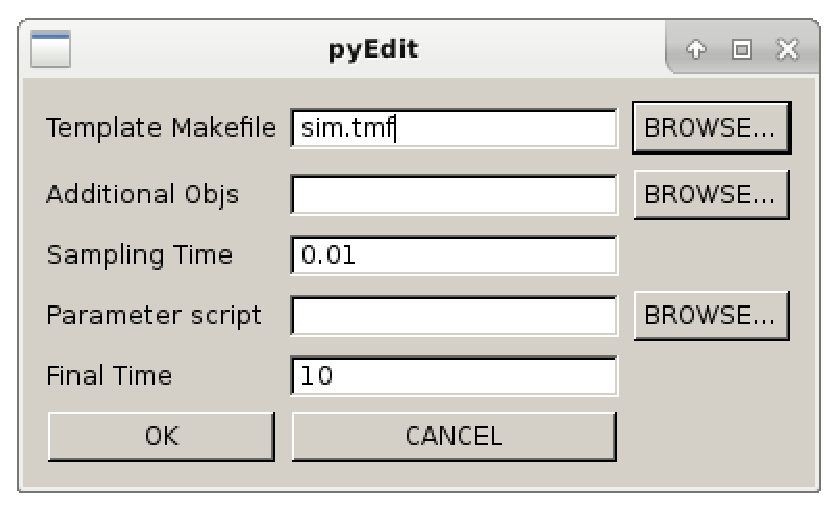
\includegraphics[width=0.4\textwidth]{gendialog.eps}
 \caption{Dialog for code generation}
 \label{codedlg}
 \end{figure}

In this dialog it is possible to choose the ``template makefile'' for 
simulation or real-time execution, the sampling time of the system and some 
additional libraries, required by special blocks.

\section{Translating the diagram into elements of the RCPdlg class}
\label{Sect-IO}

After this first setup it is possible to translate the block diagram into a 
list of elements of the class \textbf{RCPblk} provided by the 
\textbf{suspisim} package. This class contains all the information required 
for the code generation.

This class contains the following fields:

\begin{description}
\item[fcn:] the name of the C-Function to be used to handle this block
\item [pin:] an array containing the id of the input nodes
\item [pout:] an array containing the id of the output nodes
\item [nx:] the number of internal states (continuous or discrete)
\item [uy:] a flag which indicates a direct dependency between input and 
output signals (feed-through flag).
\item [realPar:] an array containing the real parameters of the block
\item [intPar:] an array containing the integer parameters of the block
\item [str:] a string related to the block
\end{description}

For example, the diagram in figure~\ref{F18} is translated into the following 
code

\begin{code}
from supsisim.RCPblk import *

STEP = stepBlk([1],  1,  1)
PM = sumBlk([1,3],[2],  [1,-1])
CSS = cssBlk([2],[3],  sys,  0)
PRINT = printBlk([1,3])

blks = [STEP,PM,CSS,PRINT,]
fname = 'step'
genCode(fname, 0.01, blks)
genMake(fname, 'sim.tmf', addObj = '')
\end{code}



\begin{figure}[htbp]	% Step
\centering
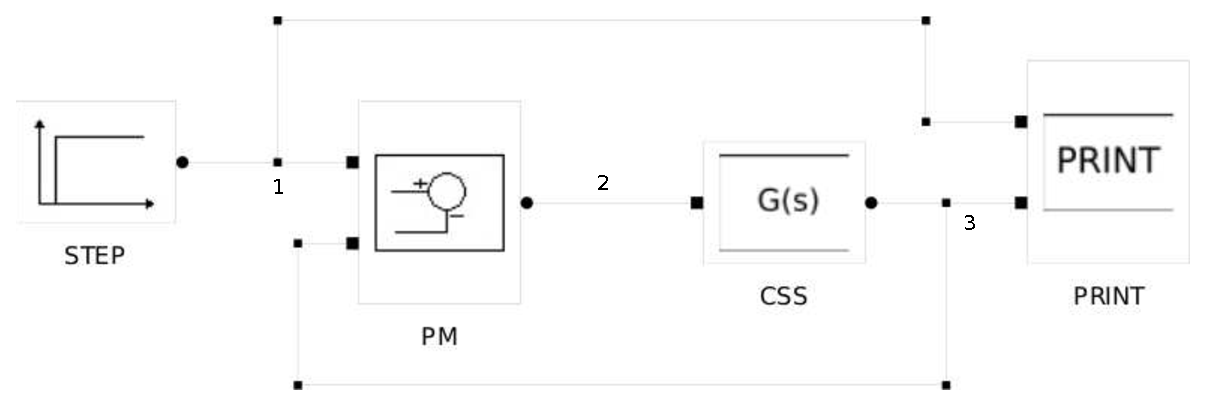
\includegraphics[width=0.8\textwidth]{eps/step1.eps}
\caption{Simple block diagram}
\label{F18}
\end{figure}

The block \textbf{CSS} has one input connected to node \ding{173} and 
one output connected to node \ding{174}, it is a continuous transfer function 
(cssBlk, $1/(s+1)$) with zero initial conditions. The \textbf{PM} block has 
2 inputs connected to node \ding{172} and \ding{174}, one output 
connected to node \ding{173} and performs a subtraction of the output from the 
input signals.

\section{Translating the block list into C-code}
\subsection{Finding the right execution sequence}
Before starting with the translation of the block diagram into C-code, we need 
to find the correct sequence of execution of the blocks. This task can be 
performed by analizing the $uy$ flag of the block object. 
When in a block the $uy$ flag is set to $1$, we need the output of the blocks 
connected at his input before starting to update his output.
This means that we have to generate a dependency tree of all the blocks and 
then we must rearrange the order of the block list for code generation.

In linear blocks for examples, the $uy$ flag is set if the $D$ matrix is not 
null.

In the blockdiagram of figure~\ref{F18}, the \textbf{PM} and the 
\textbf{PRINT} blocks require to know their inputs before update their 
outputs.

\begin{code}
In [5]: NrOfNodes = 3

In [6]: ordered_list = detBlkSeq(NrOfNodes,blks)

In [7]: for n in ordered_list:
   ...:     print n
   ...:     
Function           : css
Input ports        : [2]
Outputs ports      : [3]
Nr. of states      : [2 0]
Relation u->y      : 0
Real parameters    : [[ 0.  0. -1.  1. -1. -1.  
                        0.  0. -1.  0.  0.  0.]]
Integer parameters : [ 2  1  1  1  5  7  9 10]
String Parameter   : 

Function           : step
Input ports        : []
Outputs ports      : [1]
Nr. of states      : [0 0]
Relation u->y      : 0
Real parameters    : [1 1]
Integer parameters : []
String Parameter   : 

Function           : print
Input ports        : [1 3]
Outputs ports      : []
Nr. of states      : [0 0]
Relation u->y      : 1
Real parameters    : []
Integer parameters : []
String Parameter   : 

Function           : sum
Input ports        : [1 3]
Outputs ports      : [2]
Nr. of states      : [0 0]
Relation u->y      : 1
Real parameters    : [ 1 -1]
Integer parameters : []
String Parameter   : 
\end{code}

If the block diagram contains algebraic loops it is not possible to find a 
solution for the \textbf{detBlkSeq} function and an error is raised.

\subsection{Generating the C-code}
Starting from the ordered list of blocks, it is possible to generate 
C-code.

The code contains 3 functions:

\begin{itemize}
\item The initialization function
\item The termination function
\item The periodic task
\end{itemize}

\subsection{The init function}

In this function each block is translated into a python\_block structure 
defined as follows:

\begin{code}
typedef struct {
  int nin;             /* Number of inputs */
  int nout;            /* Number of outputs */
  int *nx;             /* Cont. and Discr states */
  void **u;            /* inputs */
  void **y;            /* outputs */
  double *realPar;     /* Real parameters */
  int *intPar;         /* Int parameters */
  char * str;          /* String */
  void * ptrPar;       /* Generic pointer */
}python_block;
\end{code}

The nodes of the block diagram are defined as ``double'' variables and the 
inputs and outputs of the blocks are defined as vectors of pointers to them.

\begin{code}
...
/* Nodes */
static double Node_1[] = {0.0};
static double Node_2[] = {0.0};
static double Node_3[] = {0.0};

/* Input and outputs */
static void *inptr_0[]  = {0};
static void *outptr_0[] = {0};
static void *outptr_1[] = {0};
static void *inptr_2[]  = {0,0};
static void *inptr_3[]  = {0,0};
static void *outptr_3[] = {0};
...
  inptr_0[0]  = (void *) Node_2;
  outptr_0[0] = (void *) Node_3;
..
  block_test[0].nin  = 1;
  block_test[0].nout = 1;
  block_test[0].nx   = nx_0;
  block_test[0].u    = inptr_0;
  block_test[0].y    = outptr_0;
...
\end{code}

After this initialization phase, the implementation functions of the blocks are 
called with the 
flag \textbf{INIT}.

\begin{code}
  css(INIT, &block_test[0]);
  step(INIT, &block_test[1]);
  print(INIT, &block_test[2]);
  sum(INIT, &block_test[3]);
\end{code}

\subsection{The termination function}
This procedure calls the implementation functions of the blocks with the flag 
\textbf{END}.

\subsection{The ISR function}
This procedure represents the periodic task of the RT execution. First of all, 
the implementation functions are called with the flag \textbf{OUT}, in order to 
perform the output update of each blocks. As a second step, the implementation 
functions of the block containing internal states ($nx \neq 0$) are called with 
the flag \textbf{STUPD} (state update).

\begin{code}
  ...
  css(OUT, &block_test[0]);
  step(OUT, &block_test[1]);
  print(OUT, &block_test[2]);
  sum(OUT, &block_test[3]);
  ...
  css(OUT, &block_test[0]);
  css(STUPD, &block_test[0]);
  ...
\end{code}

\section{The main file}

The core of the RT execution is represented by the ``python\_main\_rt.c'' file. 
During the RT execution, the main procedure starts a high priority thread for 
handling the RT behavior of the system. 
The following main file, for example, is used to launch the executable
in a Linux preempt\_rt environment.

\begin{code}
void *rt_task(void *p)
{
  ...
  param.sched_priority = prio;
  if(sched_setscheduler(0, SCHED_FIFO, &param)==-1){
    perror("sched_setscheduler failed");
    exit(-1);
  }

  ...
  double Tsamp = NAME(MODEL,_get_tsamp)();

  ...
  NAME(MODEL,_init)();

  while(!end){
   /* wait untill next shot */
    clock_nanosleep(CLOCK_MONOTONIC, 
                    TIMER_ABSTIME, &t, NULL);

    ...
    /* periodic task */
    NAME(MODEL,_isr)(T);
    ...
  }
  NAME(MODEL,_end)();  
}
\end{code}

\chapter{Example}
\section{The plant}

One of the educational plants available at the SUPSI laboratory is the system 
shown in figure~\ref{F20}. This example is located in to the 
``pycontrol/Tests/ControlDesign/DisksAndSpring'' folder,

\begin{figure}[htbp]	% Step
\centering
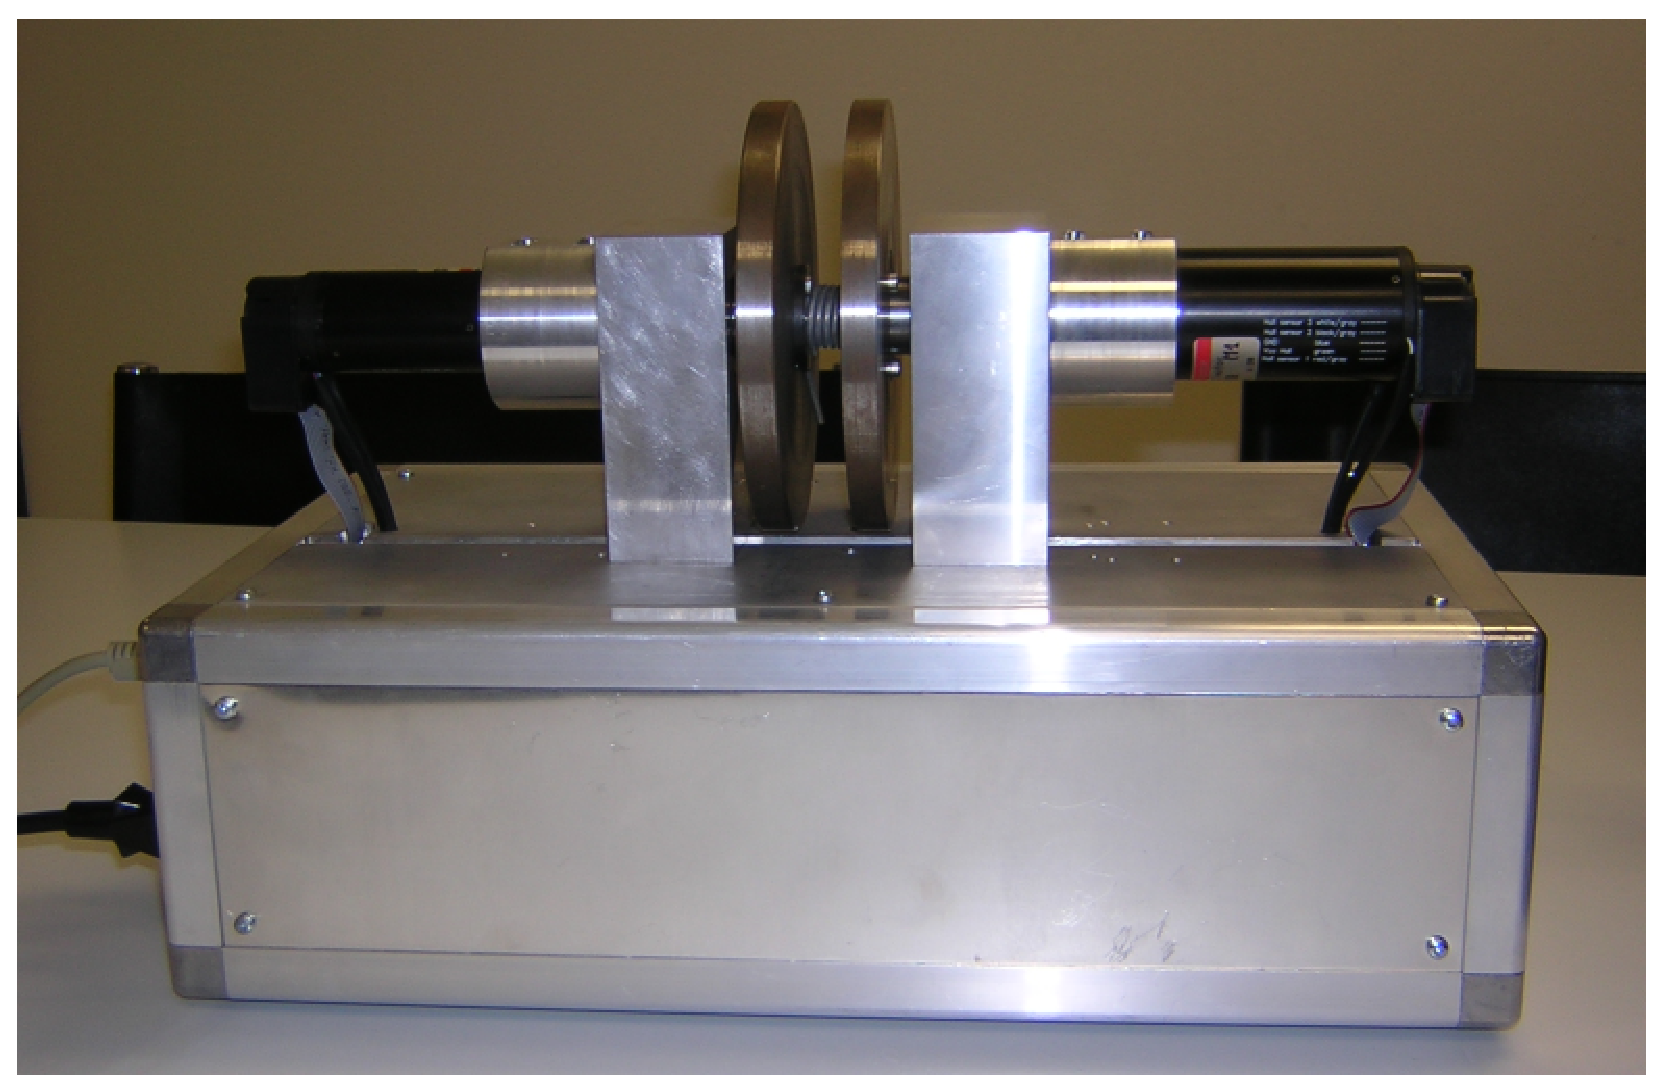
\includegraphics[width=0.6\textwidth]{eps/disks.eps}
\caption{The disks and spring plant}
\label{F20}
\end{figure}

Two disks are connected by a spring. The goal for the students is to control 
the angle of the disk on the right by applying an appropriate torque to the 
disk on the left.

The physical model of this plant can be directly calculated in python using for 
example the \textbf{sympy} toolbox.
Sympy can deliver a symbolic description of the system and through a python 
\textit{dictionary} it is possible to easily obtain the numerical matrices of 
the state-space representation of the plant.

\begin{code}

In [4]: A
Out[4]: 
matrix([[0, 0, 1, 0],
        [0, 0, 0, 1],
        [-c/J1, -c/J1, (-d - d1)/J1, -d/J1],
        [-c/J2, -c/J2, -d/J2, (-d - d2)/J2]])

In [5]: B1

Out[5]: 
matrix([[0, 0],
        [0, 0],
        [kt1/J1, 0],
        [0, kt2/J2]])

In [6]: B = B1[:,0]
        
In [7]: C
Out[7]: [[1, 0, 0, 0], [0, 1, 0, 0]]

In [8]: C2
Out[8]: [0, 1, 0, 0]

In [9]: D
Out[9]: [[0], [0]]

In [10]: D2
Out[10]: [0]
\end{code}

The control system toolbox and the additional ``yottalab.py'' package contain 
all the functions required for the design of the controller. In this case
we design a discrete-state feedback controller with integral part for 
eliminating steady-state errors. The states are estimated with a reduced-order 
observer.
In addition, an anti-windup mechanism has been implemented. The sampling time 
is set to 10 ms.

The yottalab module offers 3 functions that facilitate the controller 
design:

\begin{itemize}
\item The function \textbf{red\_obs}(sys, T, poles) which implements the 
reduced-order observer for the system \textbf{sys}, using the submatrix 
\textbf{T} (required to obtain the estimator C-matrix 
and the desired state-estimator poles \textbf{poles}.

$$
P = [C;T] \to C^*=C \cdot P^{-1}=[I_q,O_{(n-q)}]
$$

\item The function \textbf{comp\_form\_i}(sys,obs,K,Cy) that transforms the 
observer \textbf{obs} with the state-feedback gains \textbf{K} and the 
integrator part into a single dynamic block with the reference signal and the 
two positions $\varphi_1$ and $\varphi_2$ as inputs and the control current 
$I_1$ as output. The vector \textbf{Cy} is used to select $\varphi_2$ as the 
output signal that is compared with the reference signal for generating the 
steady-state error for the integral part of the controller.

\item The function \textbf{set\_aw}(sys,poles) that transforms the previous 
controller ($Contr(s)=N(s)/D(s)$) in an input state-space system and a feedback 
state-space system, implementing the anti-windup mechanism. The vector 
\textbf{poles} contains the desired poles of the two new systems ($D_{new}(s)$) 
(see figure~\ref{F20a}).

$$
sys_{in}(s) = \frac{N(s)}{D_{new}(s)} 
$$

$$
sys_{fbk}(s) = 1-\frac{D(s)}{D_{new}(s)}
$$

\end{itemize}

\begin{figure}[htbp]	% Step
\centering
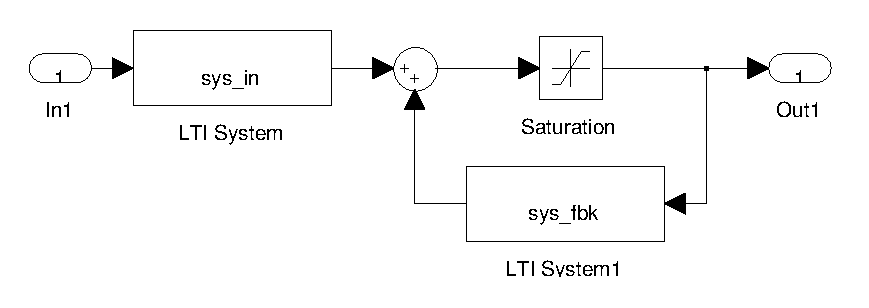
\includegraphics[width=0.8\textwidth]{eps/aw.eps}
\caption{Anti windup}
\label{F20a}
\end{figure}

\section{The plant model}

\begin{code}
# Sampling time
ts = 10e-3

gss1 = ss(A,B,C,D)
gss = ss(A,B,C2,D2)
gz = c2d(gss,ts,'zoh')
\end{code}

\section{Controller design}

\begin{code}
# Control design
wn = 10
xi1 = np.sqrt(2)/2 
xi2 = 0.85 

cl_p1 = [1,2*xi1*wn,wn**2]
cl_p2 = [1,2*xi2*wn,wn**2]
cl_p3 = [1,wn]
cl_poly1 = sp.polymul(cl_p1,cl_p2)
cl_poly = sp.polymul(cl_poly1,cl_p3)
cl_poles = sp.roots(cl_poly)     # Desired continuous poles
cl_polesd = sp.exp(cl_poles*ts)  # Desired discrete poles

# Add discrete integrator for steady state zero error
Phi_f = np.vstack((gz.A,-gz.C*ts))
Phi_f = np.hstack((Phi_f,[[0],[0],[0],[0],[1]]))
G_f = np.vstack((gz.B,zeros((1,1))))

# Pole placement
k = placep(Phi_f,G_f,cl_polesd)
\end{code}

\section{Observer design}
\begin{code}
# Observer design - reduced order observer
poli_o = 5*cl_poles[0:2]
poli_oz = sp.exp(poli_o*ts) 

disks = ss(A,B,C,D)
disksz = StateSpace(gz.A,gz.B,C,D,ts)
T = [[0,0,1,0],[0,0,0,1]]

# Reduced order observer
r_obs = red_obs(disksz ,T, poli_oz)

# Controller and observer in the same matrix -  Compact form
contr_I = comp_form_i(disksz,r_obs,k,[0,1])

# Implement anti windup
[gss_in,gss_out] = set_aw(contr_I,[0.1,0.1,0.1])
\end{code}

\section{Simulation}

We can perform the simulation of the discrete-time controller with the 
continuous-time mathematic plant model using the block diagram of 
figure~\ref{F21}

\begin{figure}[htbp]	% Step
\centering
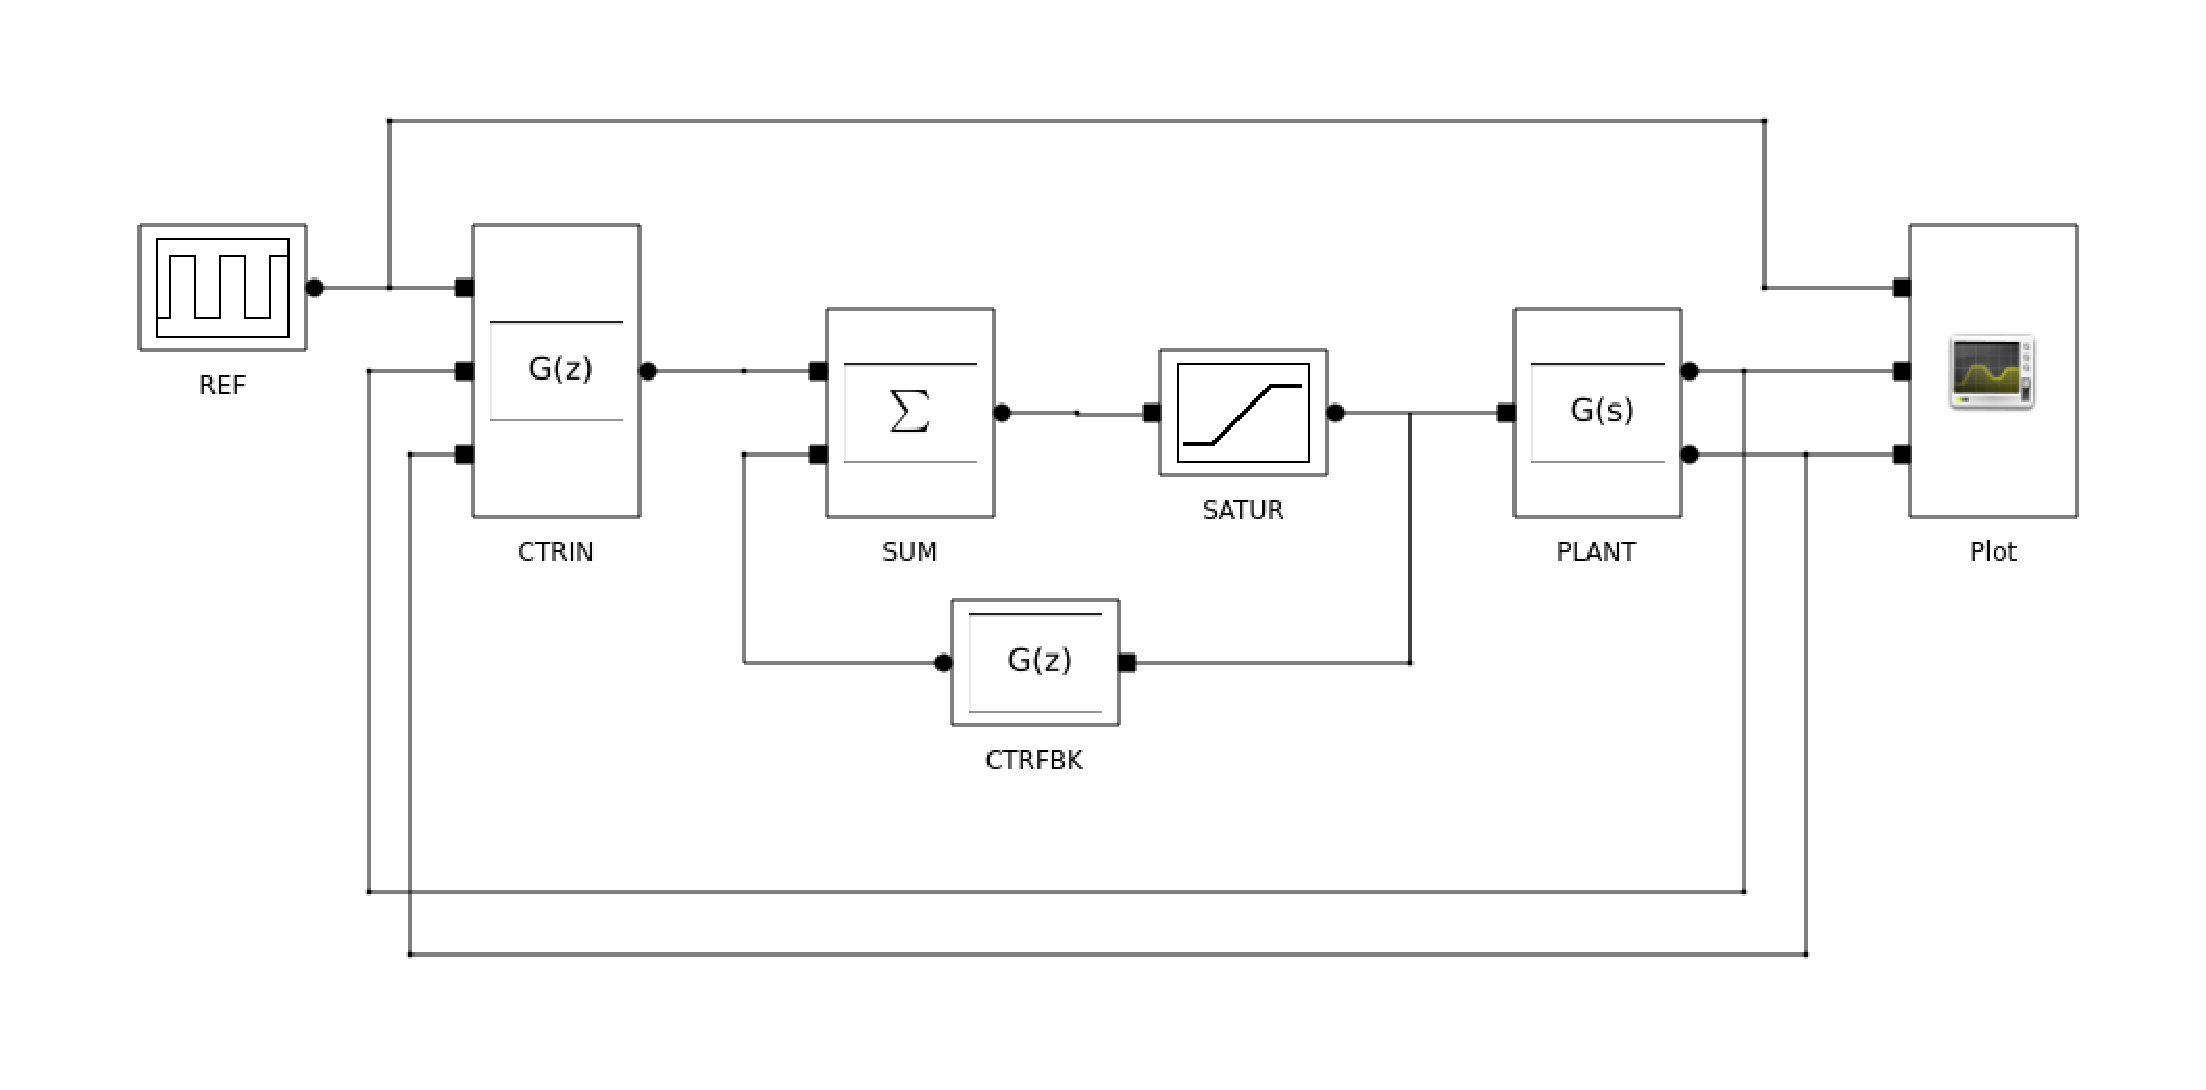
\includegraphics[width=0.9\textwidth]{eps/diskssim.eps}
\caption{Block diagram for the simulation}
\label{F21}
\end{figure}

This diagram is stored as ``disks\_sim.dgm'' in the folder.

The plant is represented by a continuous-time state-space block with 1 input 
and 2 outputs.
The controller implements the state-feedback gains and the state observer 
and it has been split into a CTRIN block and a CTRFBK block in order to 
implement the anti-windup mechanism.

Now we can launch the simulation with the command ``Simulate'' from the toolbar 
or from the menu.

A double click on the `block ``Plot'' show the result of the simulation (see 
figure~\ref{F22})

\begin{figure}[htbp]	% Step
\centering
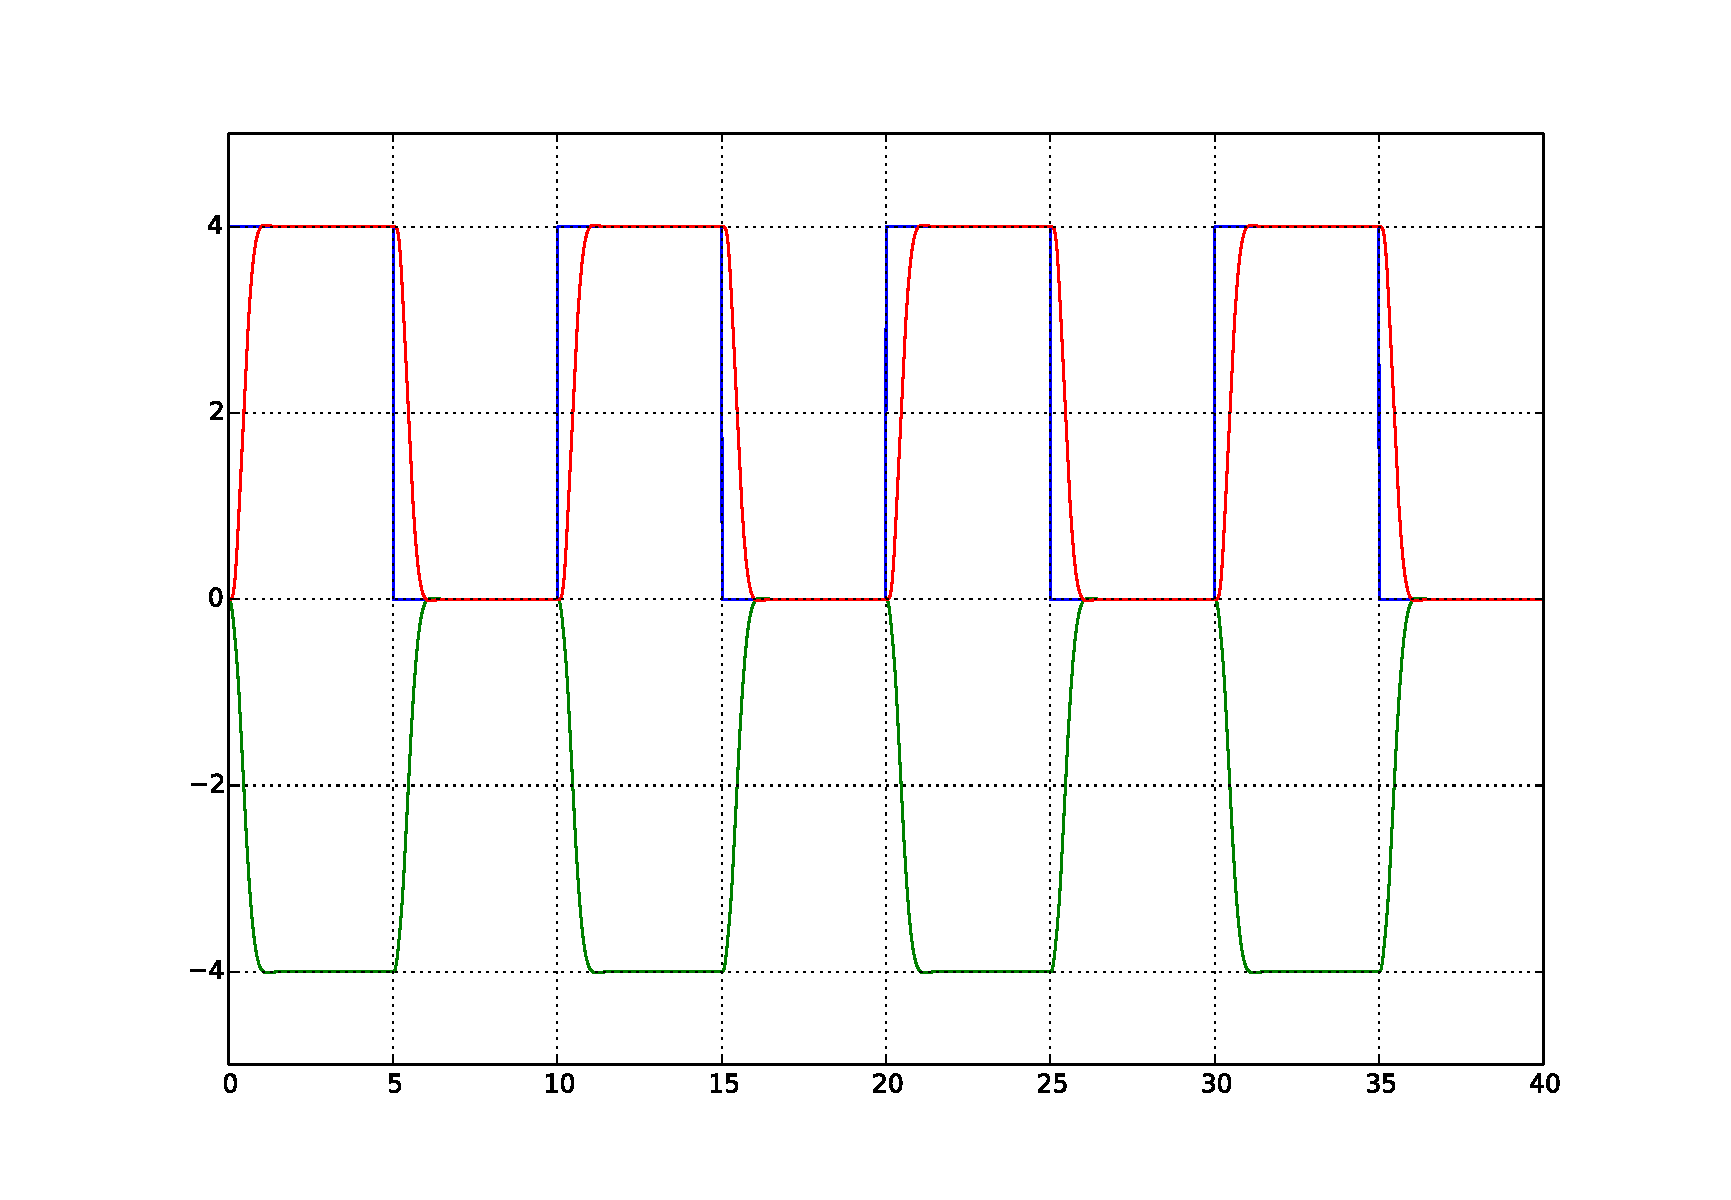
\includegraphics[width=0.8\textwidth]{eps/simout.eps}
\caption{Simulation of the plant}
\label{F22}
\end{figure}

\section{Real-time controller}

In order to generate the RT controller for the real plant, we first have to 
substitute the plant with the interfaces for sensors and actuators using blocks 
that send and receive CAN message using a USB dongle of Peak System. The 
template makefile for this system is now \textbf{rt.tmf}, that allows to 
generate code with real-time behaviour.

The block diagram for the real-time controller is represented in 
figure~\ref{F23}.

\begin{figure}[htbp]	% Step
\centering
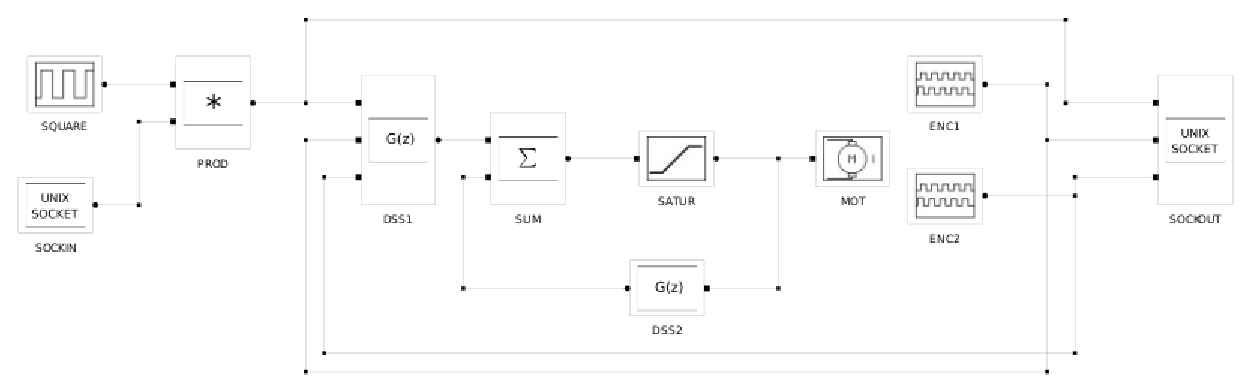
\includegraphics[width=0.9\textwidth]{eps/disksrt.eps}
\caption{Block diagram for the RT implementation}
\label{F23}
\end{figure}

The motor position can be plotted in python at the end of the execution (see 
figure~\ref{F24}).

\begin{figure}[htbp]	% Step
\centering
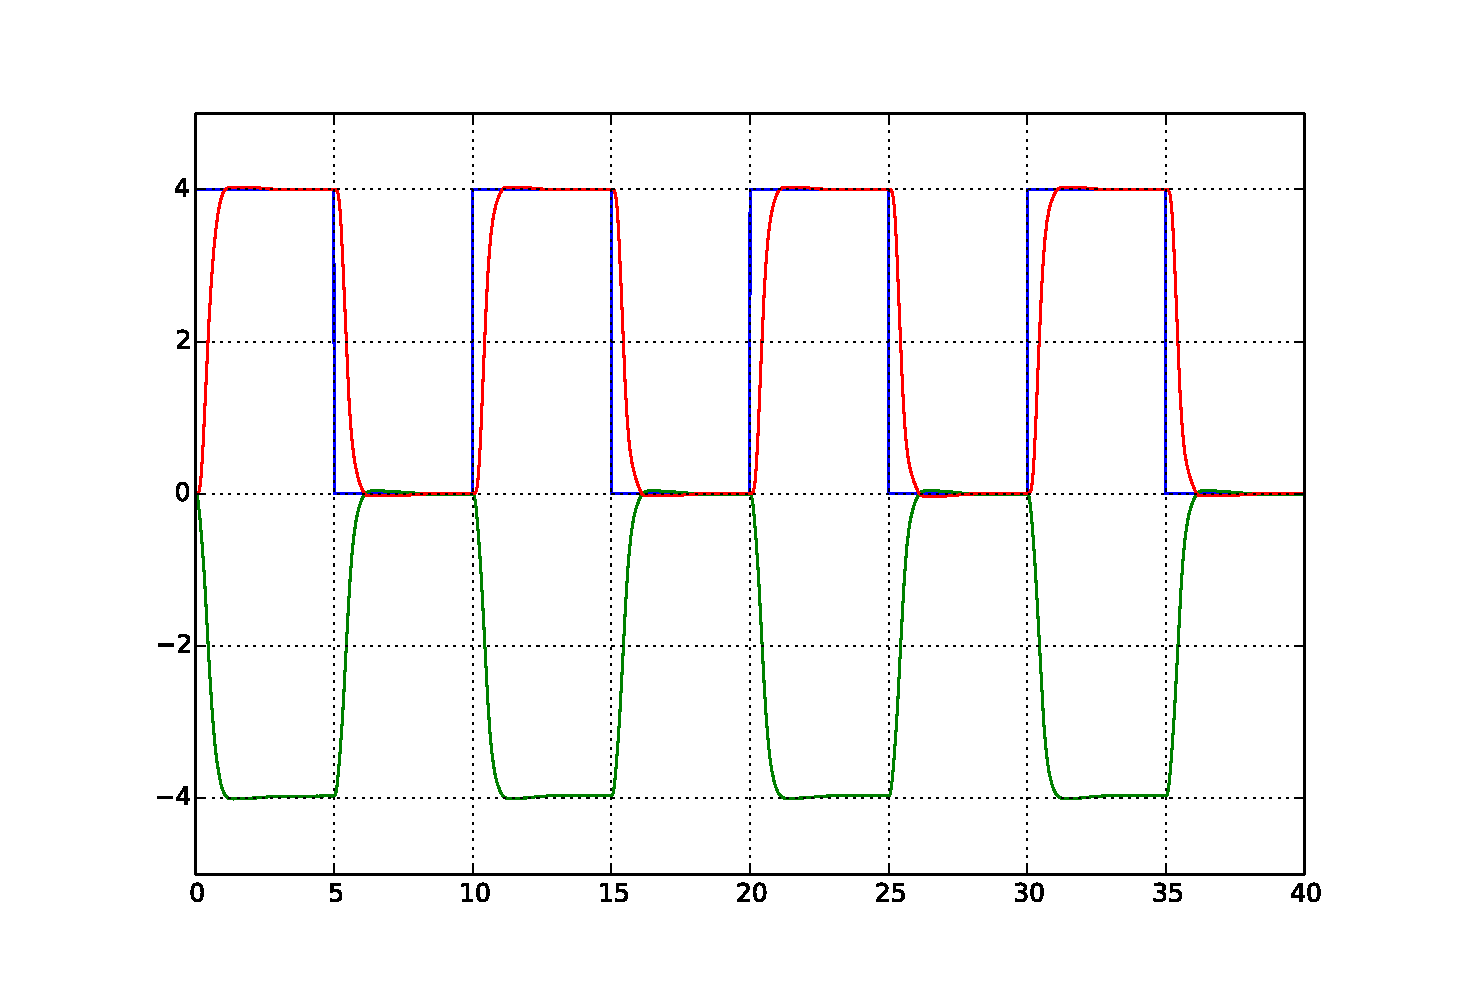
\includegraphics[width=0.7\textwidth]{eps/rtout.eps}
\caption{RT execution}
\label{F24}
\end{figure}
